\section{System Modeling \& Diagrams}
\subsection{Event Table}

\small 
\setlength{\tabcolsep}{4pt} 
\renewcommand{\arraystretch}{1.5} 

\begin{xltabular}{\textwidth}{|>{\centering\arraybackslash}p{0.7cm}|Y|Y|>{\centering\arraybackslash}p{1.7cm}|Y|Y|>{\centering\arraybackslash}p{1.8cm}|}
    \hline
    \textbf{\#} & \centering\textbf{EVENT NAME} & \centering\textbf{TRIGGER} & \textbf{SOURCE} & \centering\textbf{USE CASE} & \centering\textbf{RESPONSE} & \textbf{DEST.} \\ \hline
    \endfirsthead 

    1 & Developer login to the system & 
    \begin{tabitem}
        \item Developer's Info
        \item Login request
    \end{tabitem} & Developer & Login Developer & 
    \begin{tabitem}
        \item Show dashboard
        \item Error if login fails
    \end{tabitem} & Developer \\ \hline
    
    2 & Developer Update profile & 
    \begin{tabitem}
        \item Developer Id
        \item Details info
    \end{tabitem} & Developer & Update profile & 1. Updated profile & Developer \\ \hline
    
    3 & Developer creates a new project & 
    \begin{tabitem}
        \item New Project Request
        \item Details (name, DB)
    \end{tabitem} & Developer & Create a new Project & 
    \begin{tabitem}
        \item Nav to Schema Tab
        \item Save project records
    \end{tabitem} & Developer \\ \hline
    
    4 & Developer deletes project & 1. Project Id & Developer & Delete Exist Project & 1. Updated List of projects & Developer \\ \hline
    
    5 & Create project schema & 
    \begin{tabitem}
        \item Schema Gen. request
        \item Natural language
    \end{tabitem} & Developer & Create Schema & 1. Visualize Generated Schema & Developer \\ \hline
    
    6 & Developer modifies Entities & 
    \begin{tabitem}
        \item Entities info
        \item Create/Edit Entities
    \end{tabitem} & Developer & Modify Entities & 
    \begin{tabitem}
        \item Query response msg
        \item Update Entity in DB
    \end{tabitem} & Developer \\ \hline
    
    7 & Developer executes query & 
    \begin{tabitem}
        \item Query statement
        \item Project Id
    \end{tabitem} & Developer & Execute Query & 
    \begin{tabitem}
        \item Query response msg
        \item Show results
    \end{tabitem} & Developer \\ \hline
    
    8 & Developer modifies data & 
    \begin{tabitem}
        \item CRUD request
        \item Project Id
    \end{tabitem} & Developer & CRUD operations & 
    \begin{tabitem}
        \item Response message
        \item Updated DB
    \end{tabitem} & Developer \\ \hline
    
    
    9 & Developer Requests Restore & 1. Restore Request (Select Point-in-Time) & Developer & Restore Project & 1. Restore requested backup & Developer \\ \hline
    
    10 & Developer Upgrades Tier & 1. Subscription Change Request & Developer & Manage Subscription & 1. Update Tenant Quotas & Developer \\ \hline

    11 & Developer forgets password & 
    \begin{tabitem}
        \item Email address
        \item Reset request
    \end{tabitem} & Developer & Forget Password & 
    \begin{tabitem}
        \item Send reset link
        \item Update password
    \end{tabitem} & Developer \\ \hline
    
    12 & Developer deletes account & 
    \begin{tabitem}
        \item Delete request
        \item Verification
    \end{tabitem} & Developer & Delete Account & 1. Permanent deletion of data & Developer \\ \hline

\caption{System Event Table}
\label{table:system_event_table}
\end{xltabular}
%%%%%%%%%%%%%%%%%%%%%%%%%%%%%%%%%%%%%%%%%
%           Activity Diagrams           %
%%%%%%%%%%%%%%%%%%%%%%%%%%%%%%%%%%%%%%%%%
\subsection{Activity Diagrams}
    \begin{figure}[H]
        \centering
        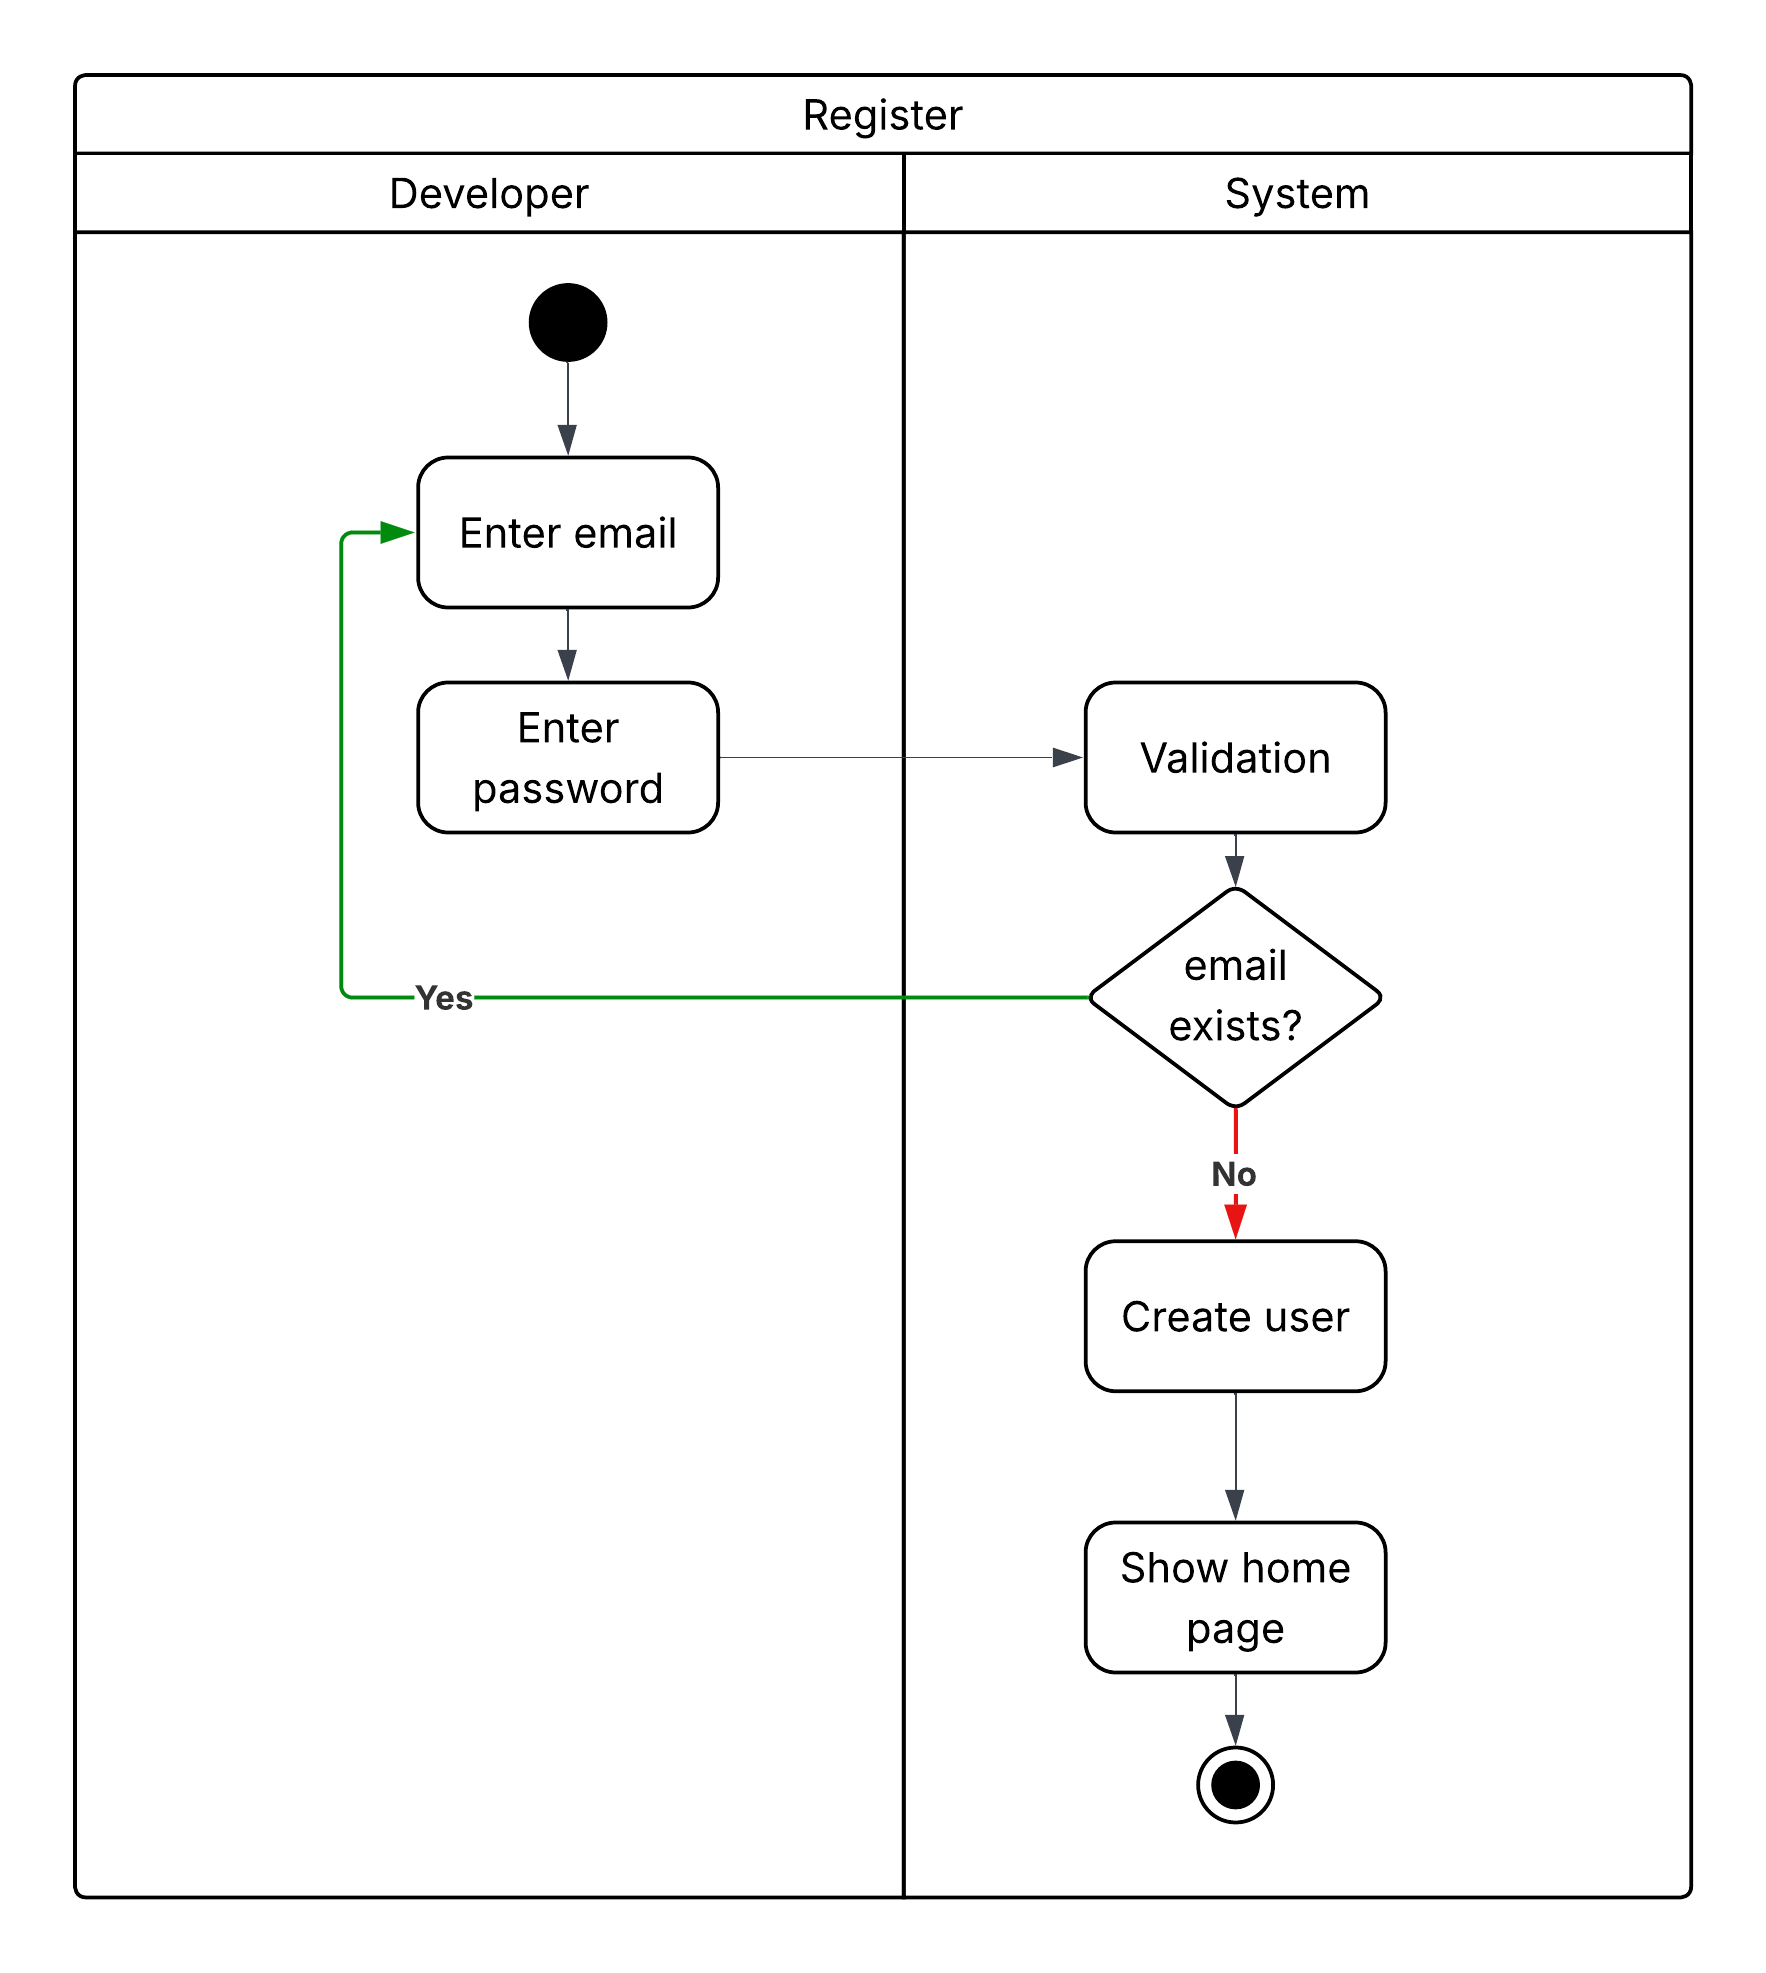
\includegraphics{images/activity/register_activity_diagram.png}
        \caption{Register activity diagram}
        \label{fig:register_activity}
    \end{figure}
    
    \begin{figure}[H]
        \centering
        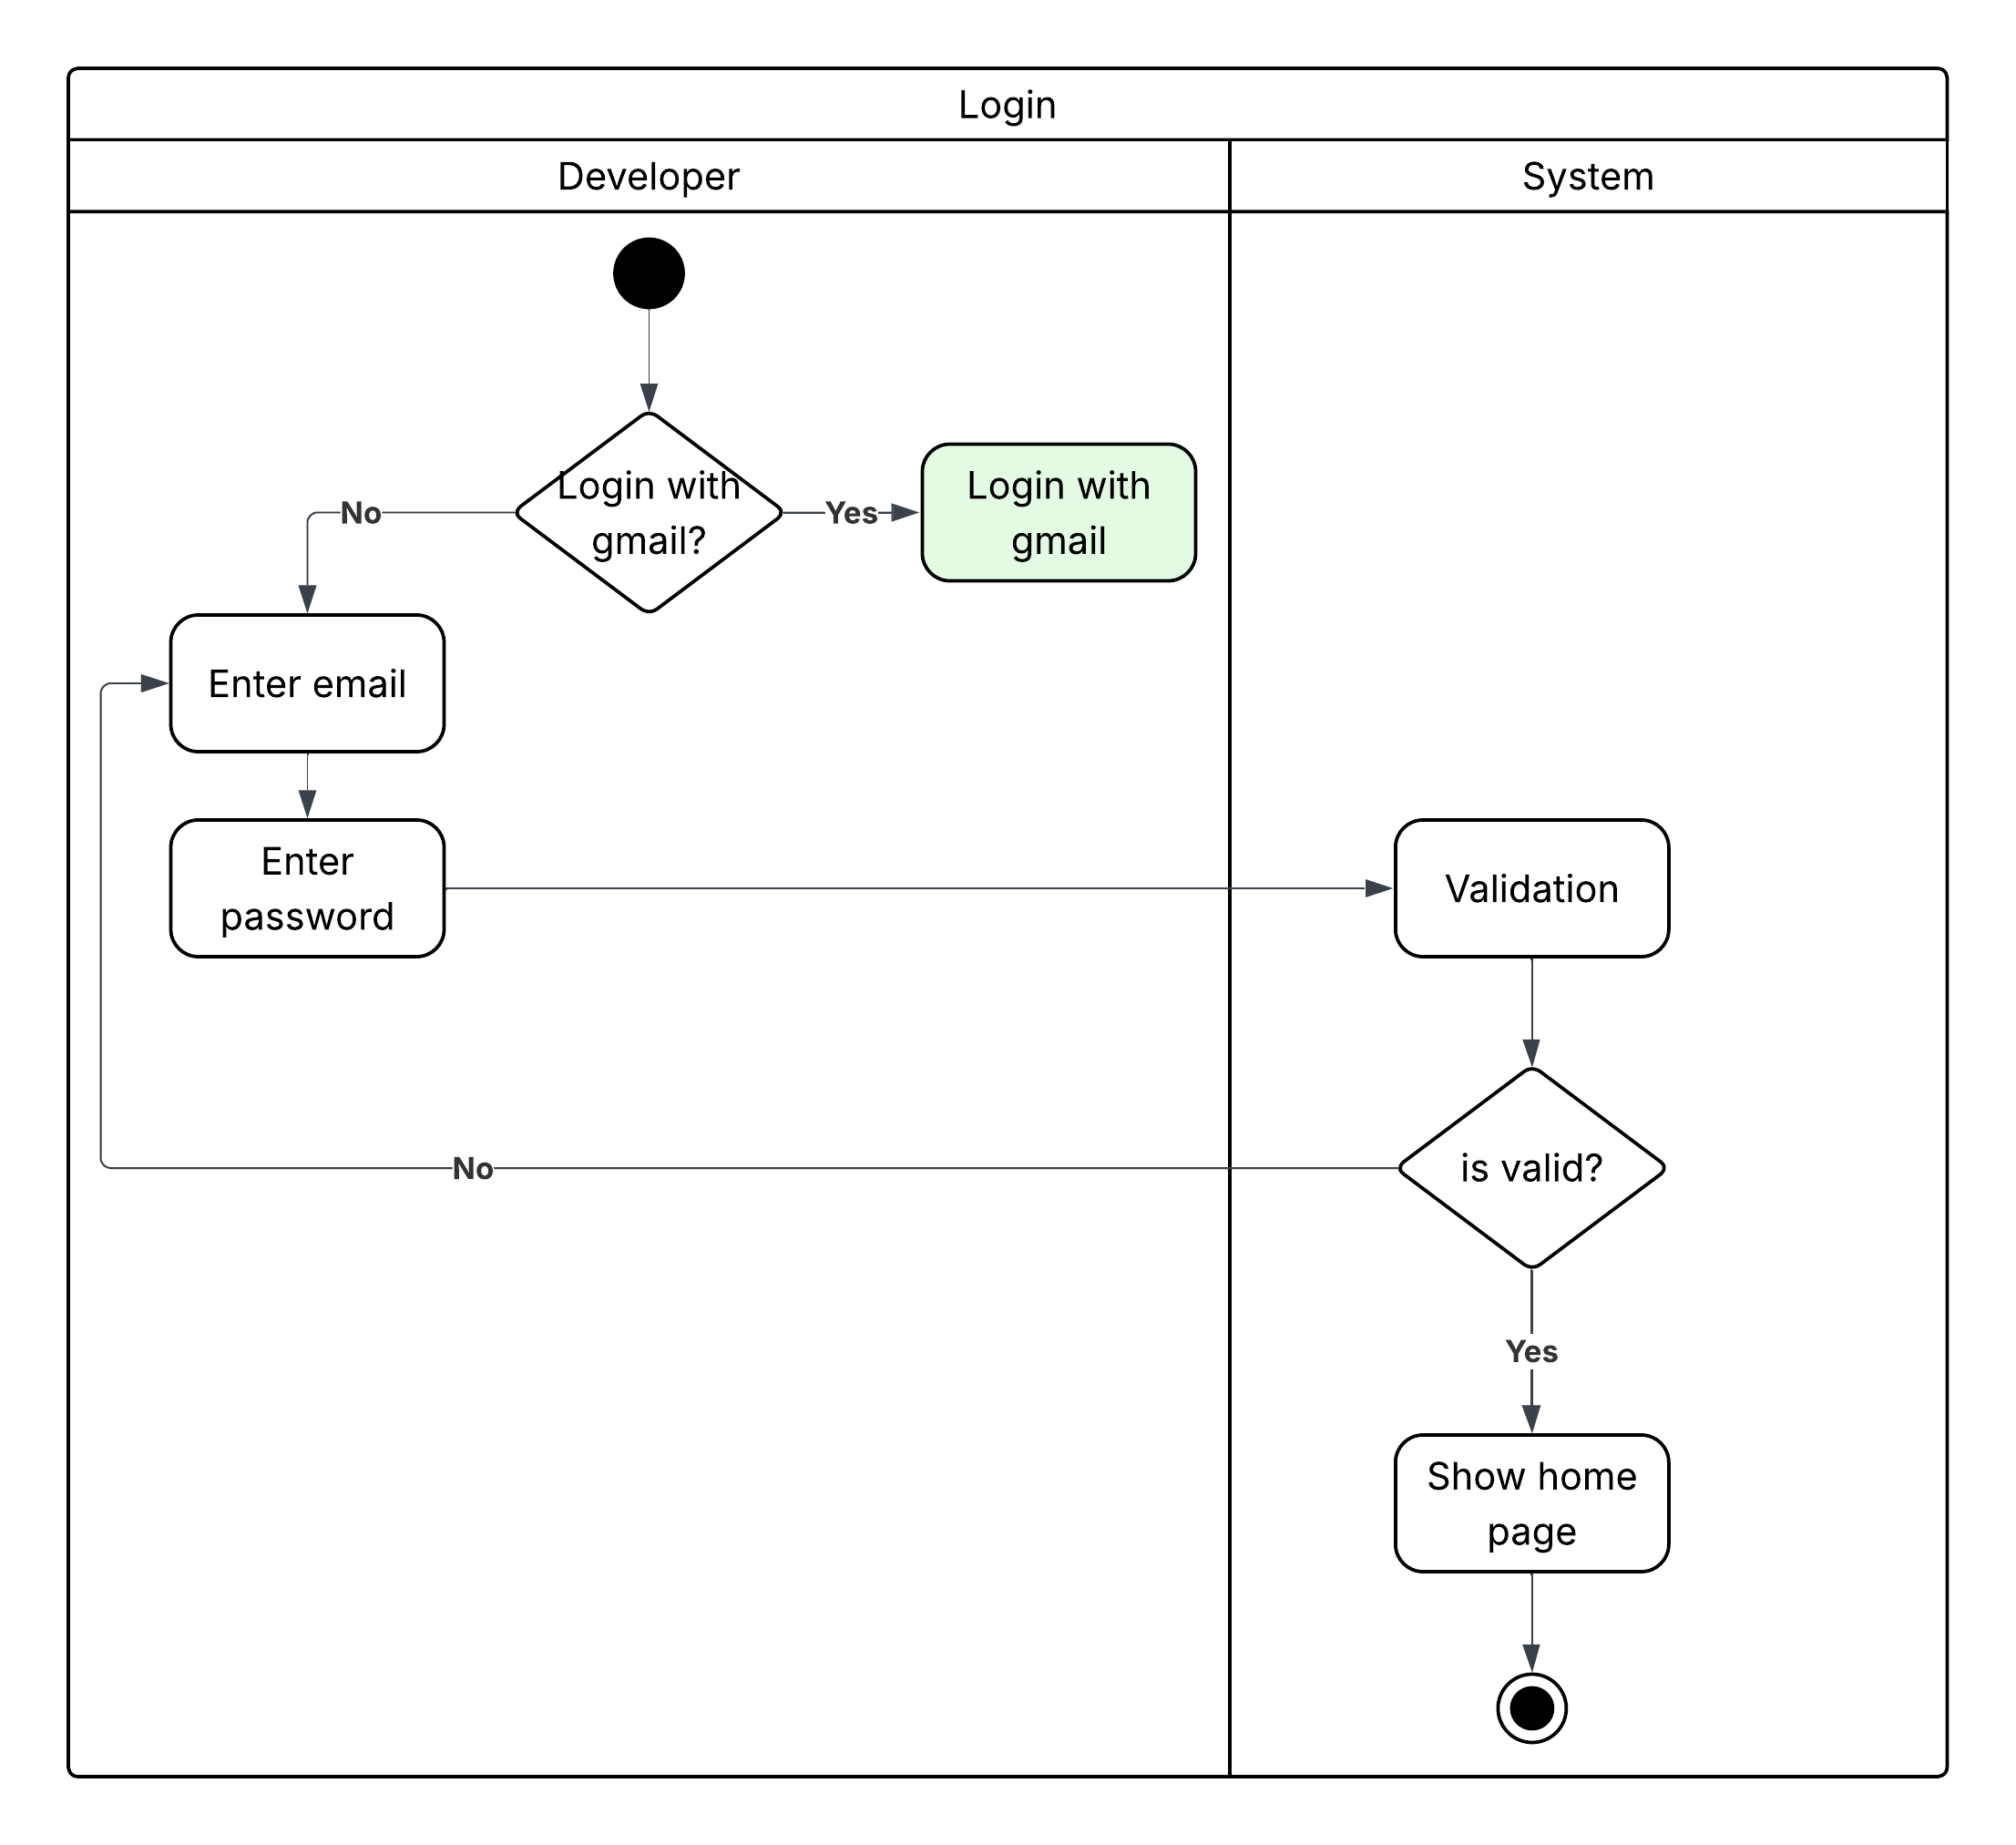
\includegraphics{images/activity/login_activity_diagram.png}
        \caption{Login activity diagram}
        \label{fig:login_activity}
    \end{figure}
    
    \begin{figure}[H]
        \centering
        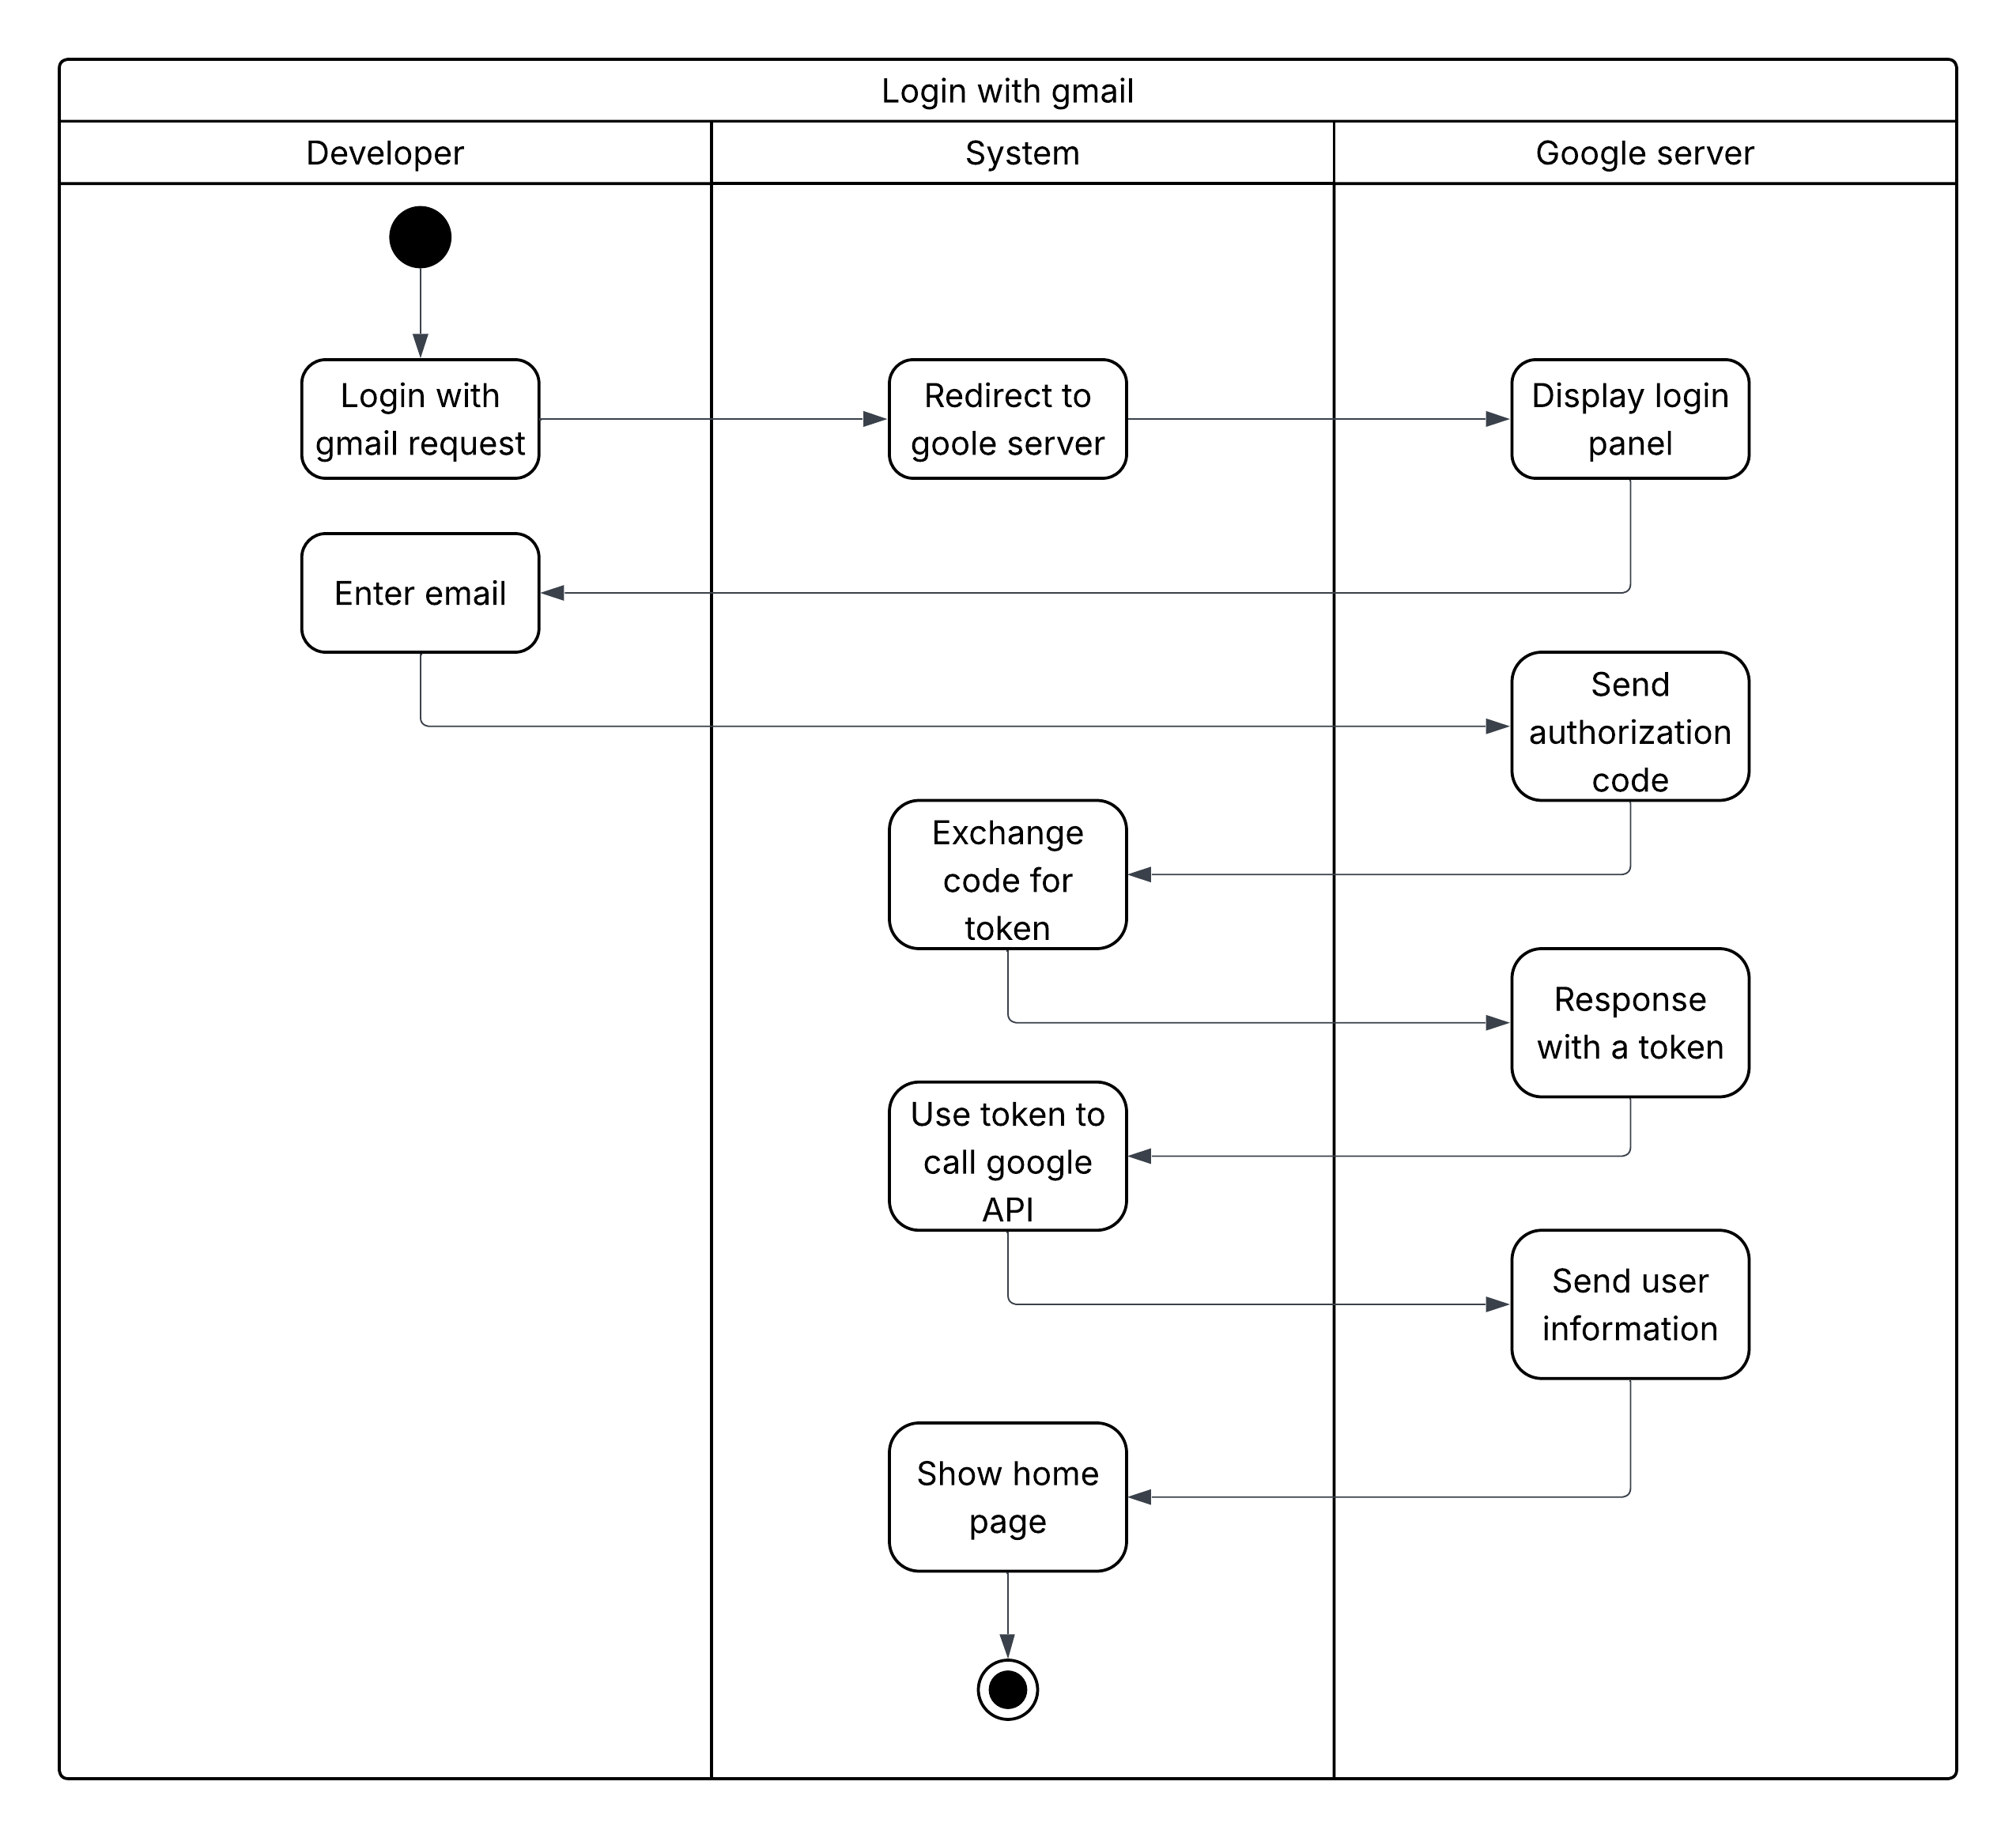
\includegraphics{images/activity/login_with_gmail_activity.png}
        \caption{Login with g-mail activity diagram}
        \label{fig:login_with_gmail_activity}
    \end{figure}

    \begin{figure}[H]
        \centering
        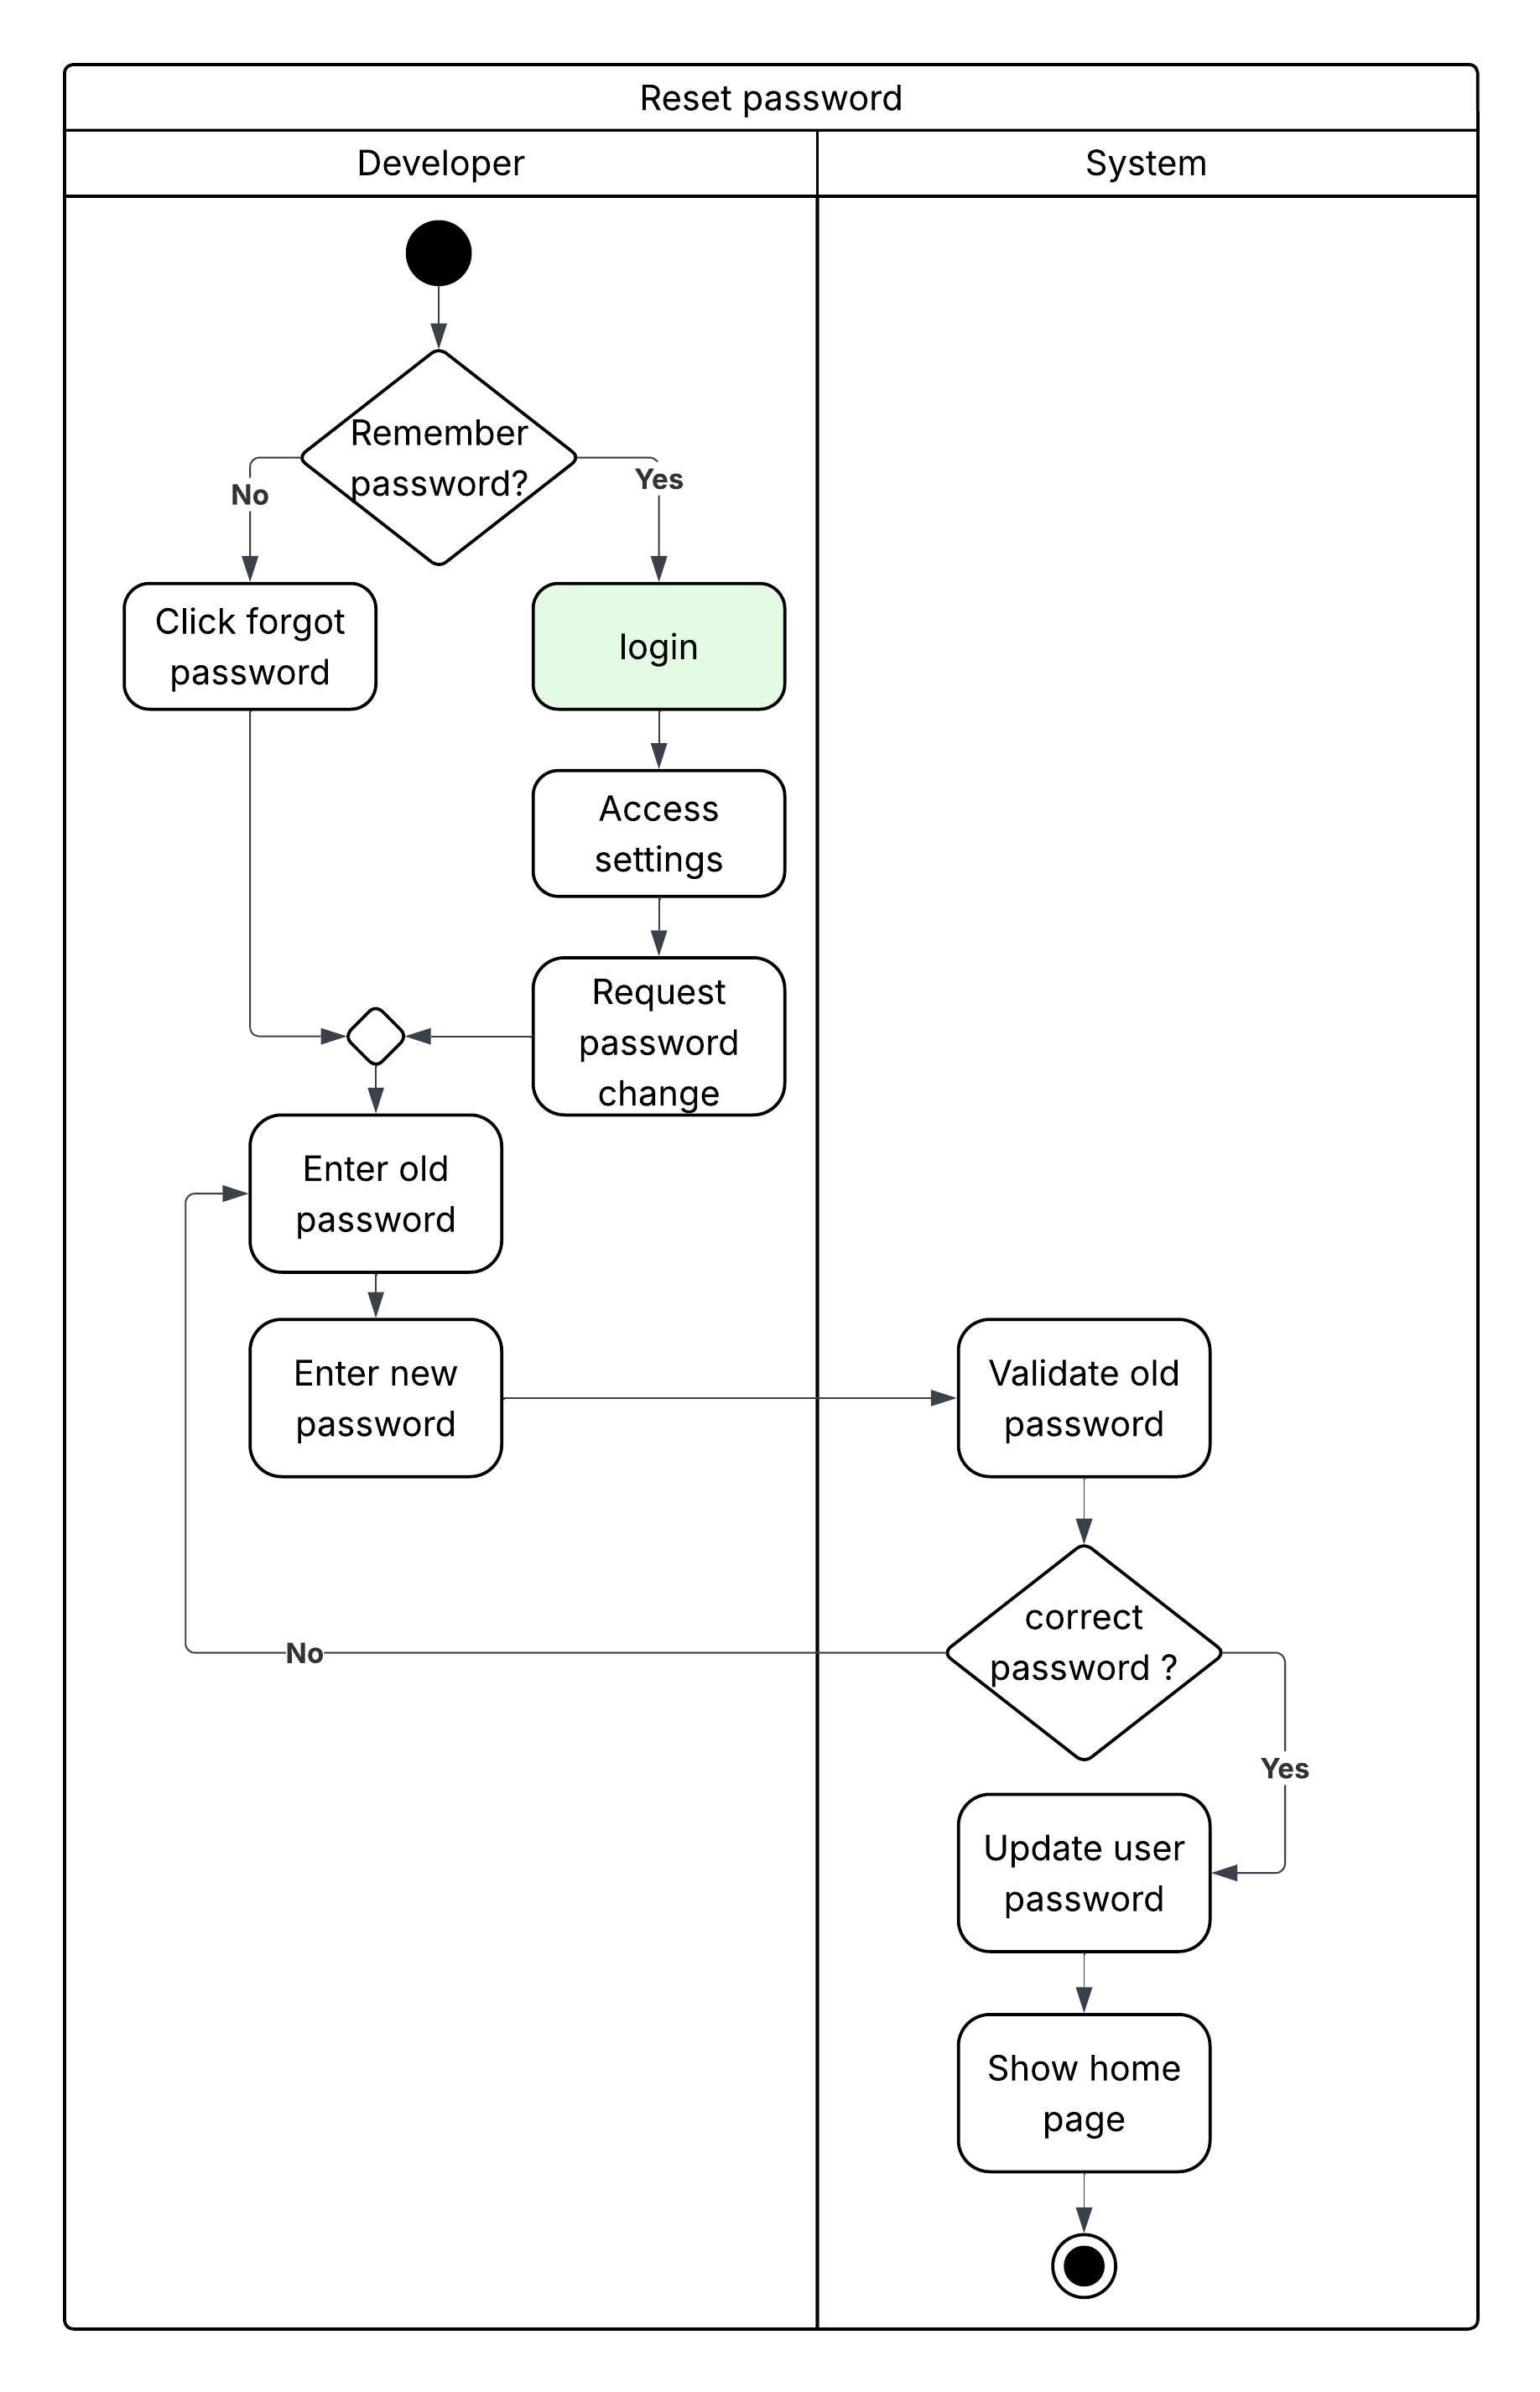
\includegraphics[height=0.95\textheight]{images/activity/reset_password_activity.png}
        \caption{Reset password activity diagram}
        \label{fig:reset_password_activity}
    \end{figure}
    
   \begin{figure}[H]
        \centering
        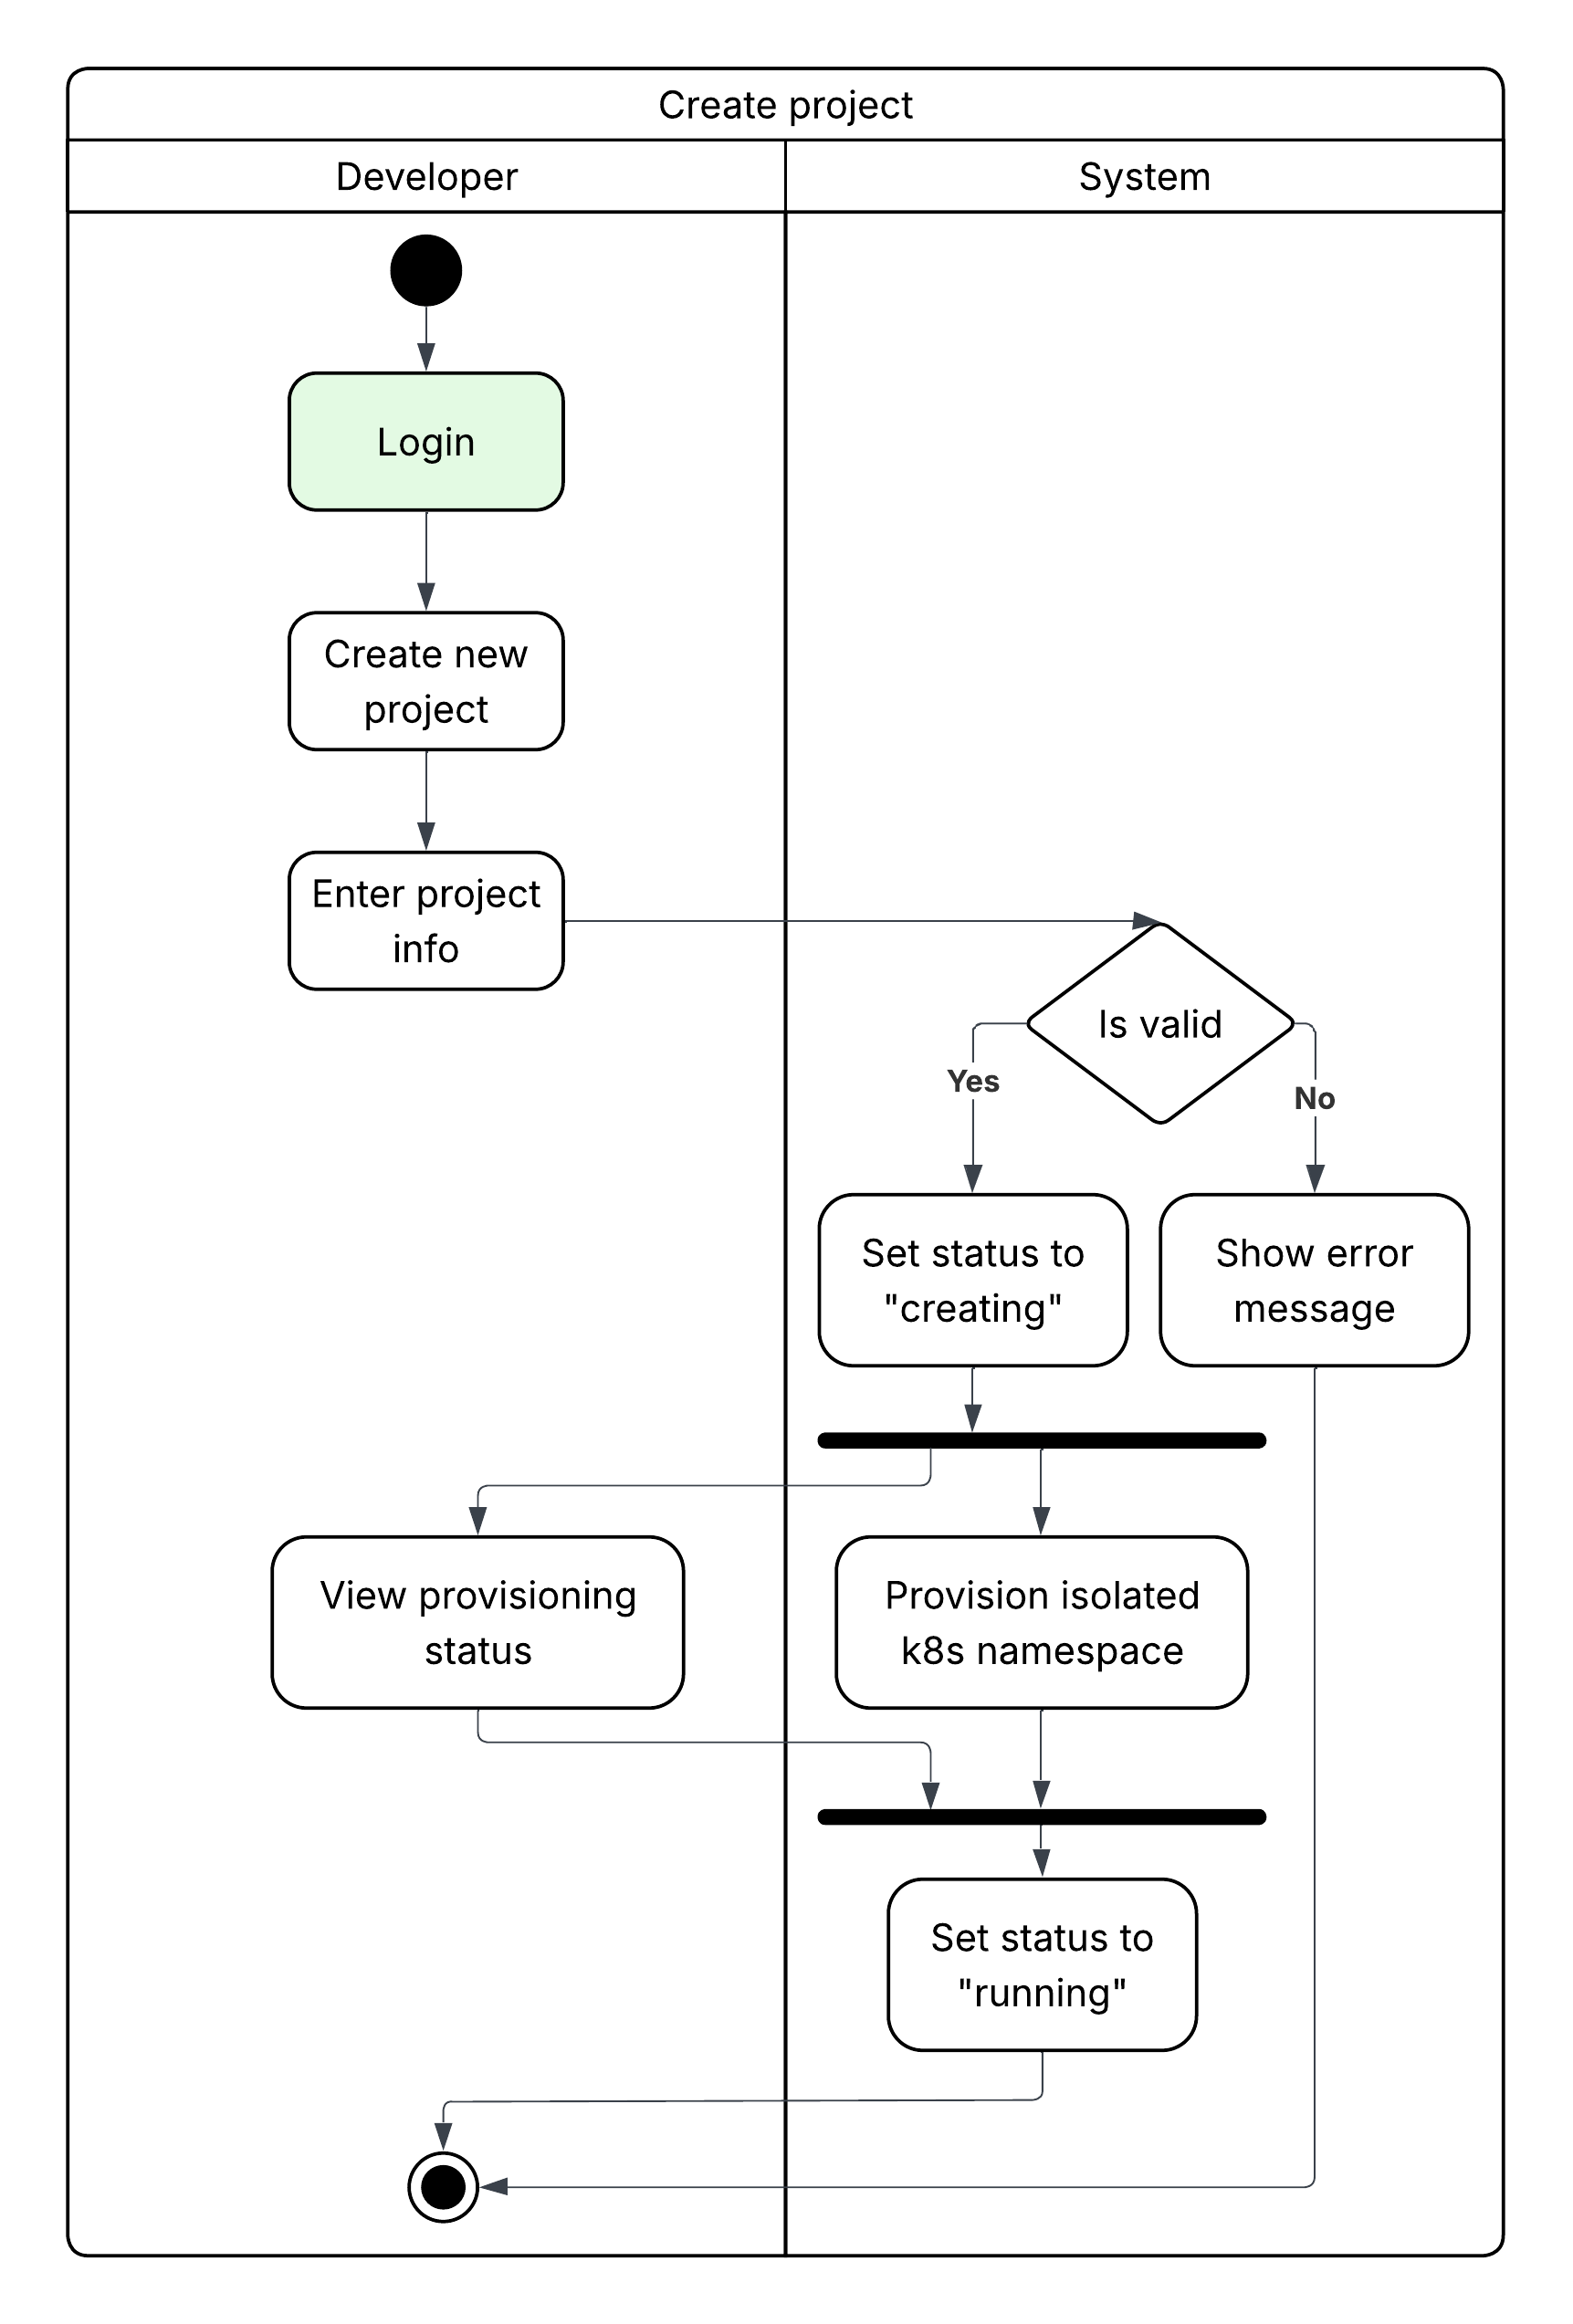
\includegraphics{images/activity/23.Create_Project.png}
        \caption{Create project activity diagram}
        \label{fig:create_project_activity}
    \end{figure}
    
    \begin{figure}[H]
        \centering
        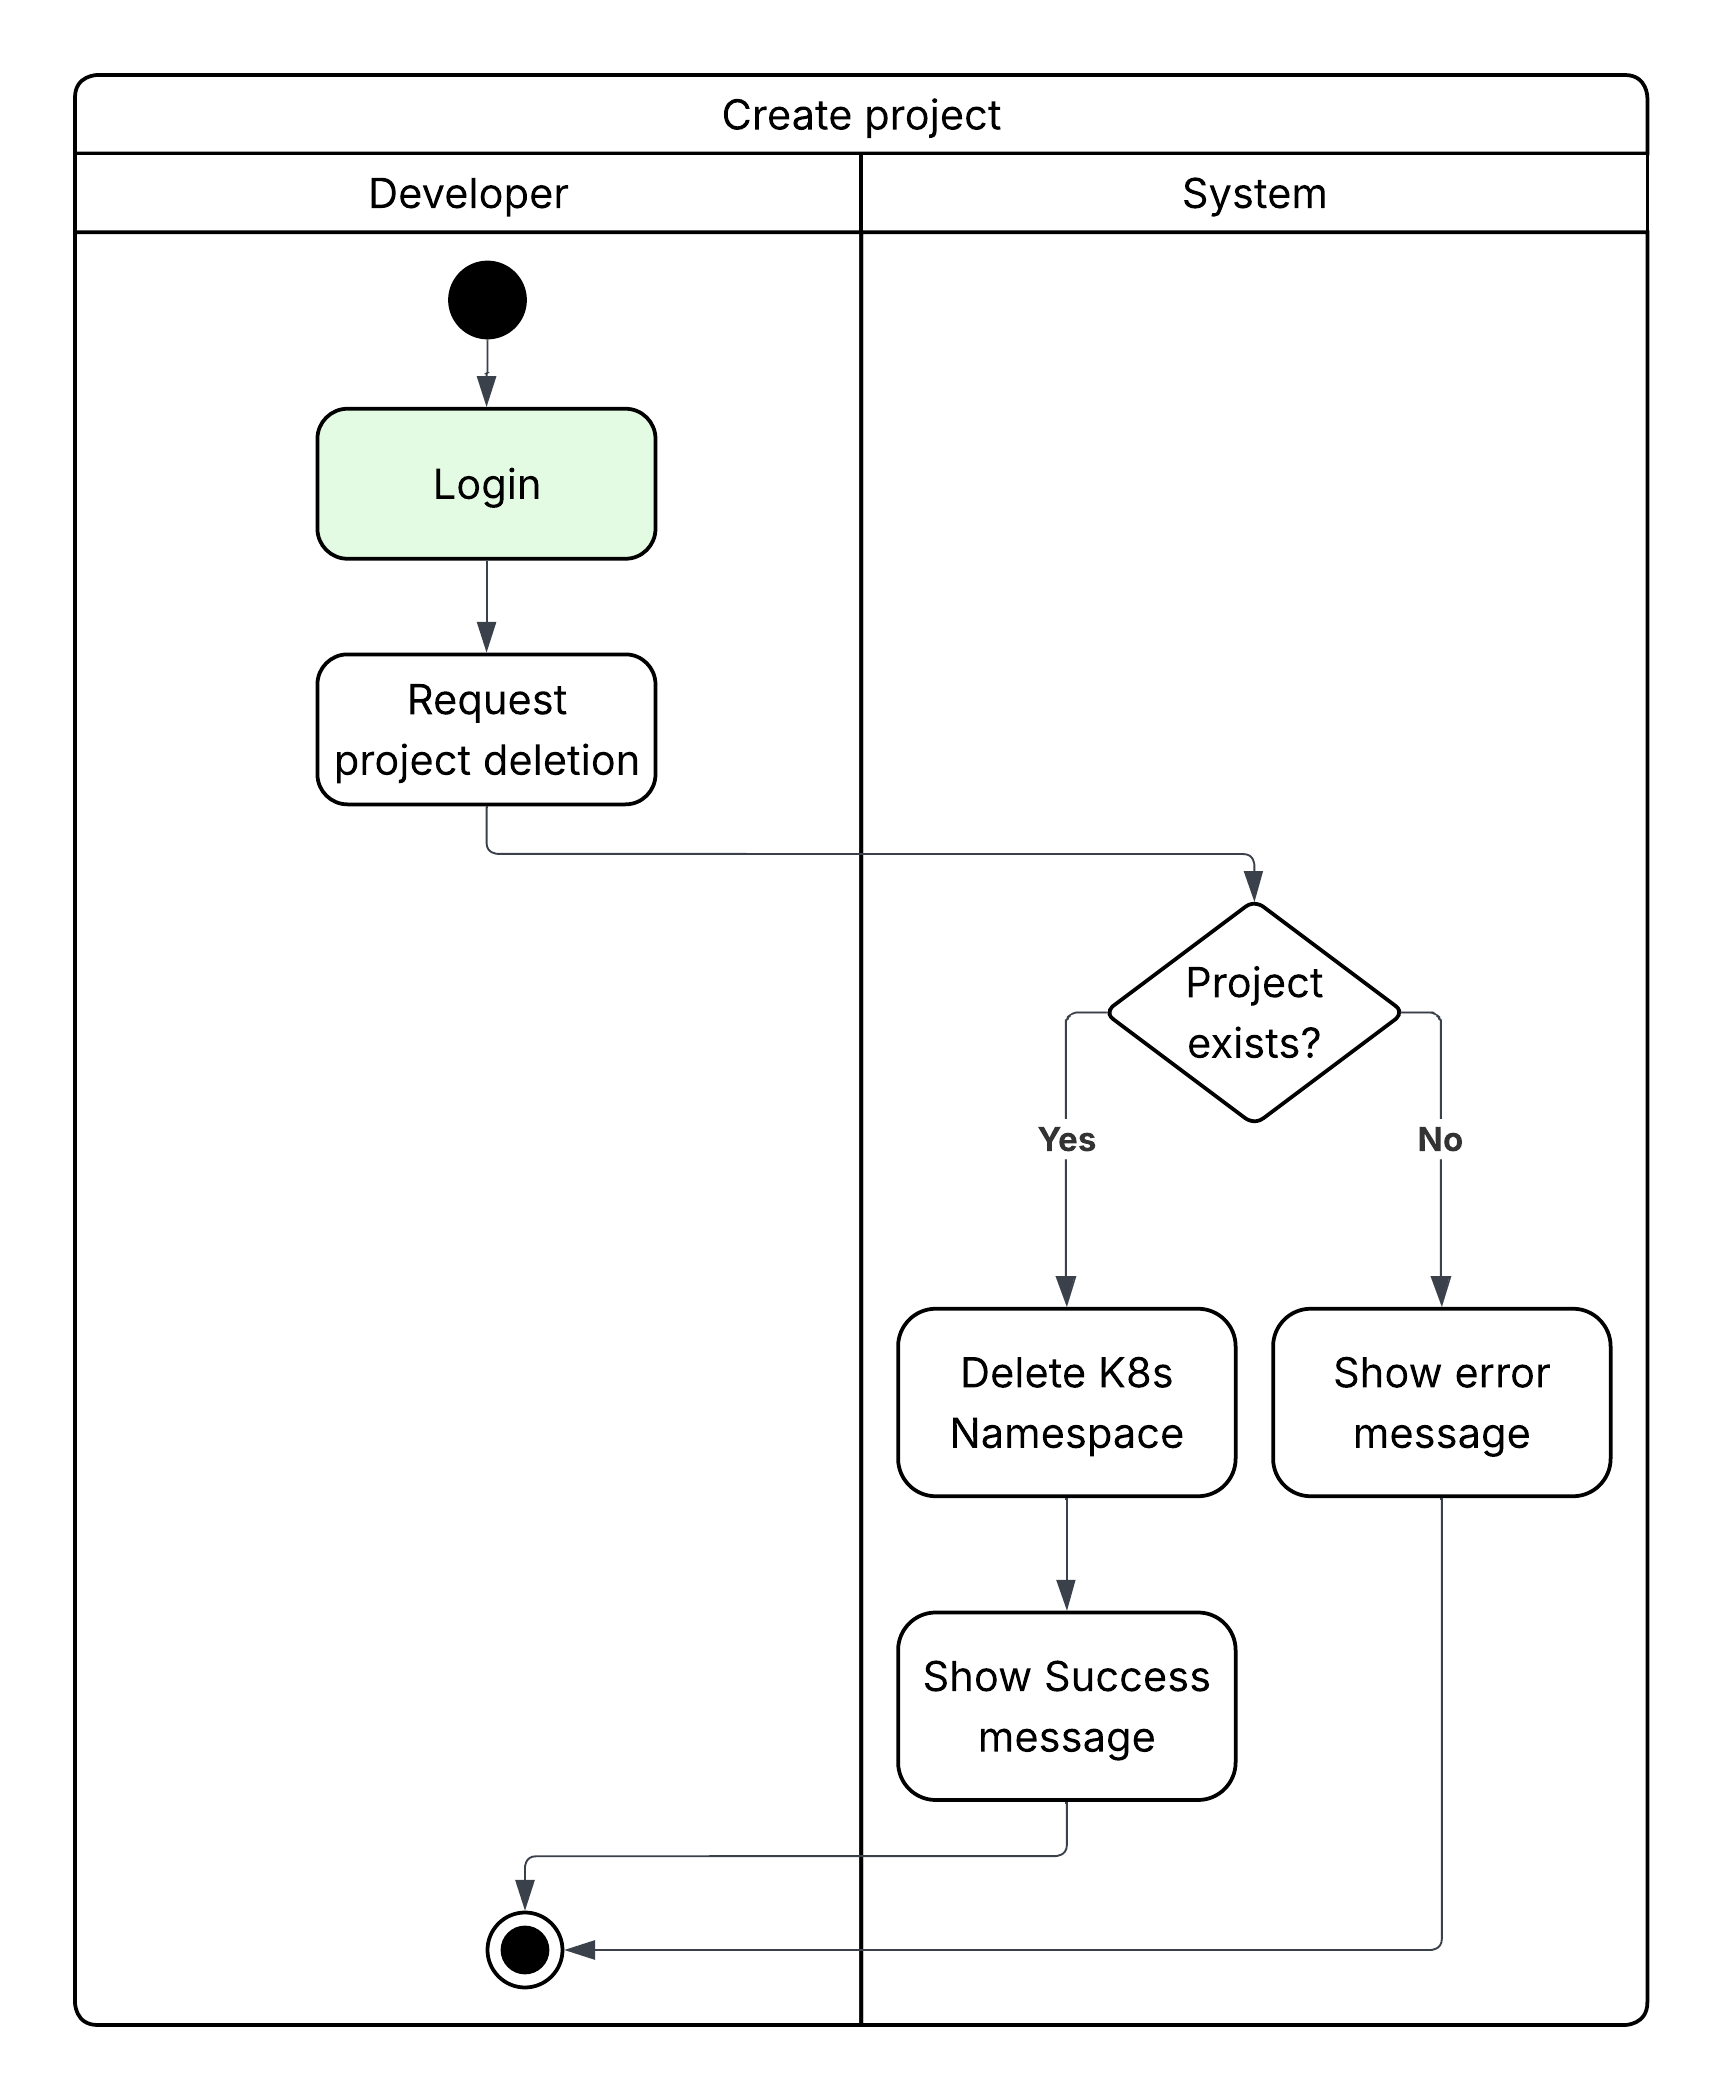
\includegraphics{images/activity/24.Delete_Database.png}
        \caption{Delete project activity diagram}
        \label{fig:delete_project_activity}
    \end{figure}

    \begin{figure}[H]
        \centering
        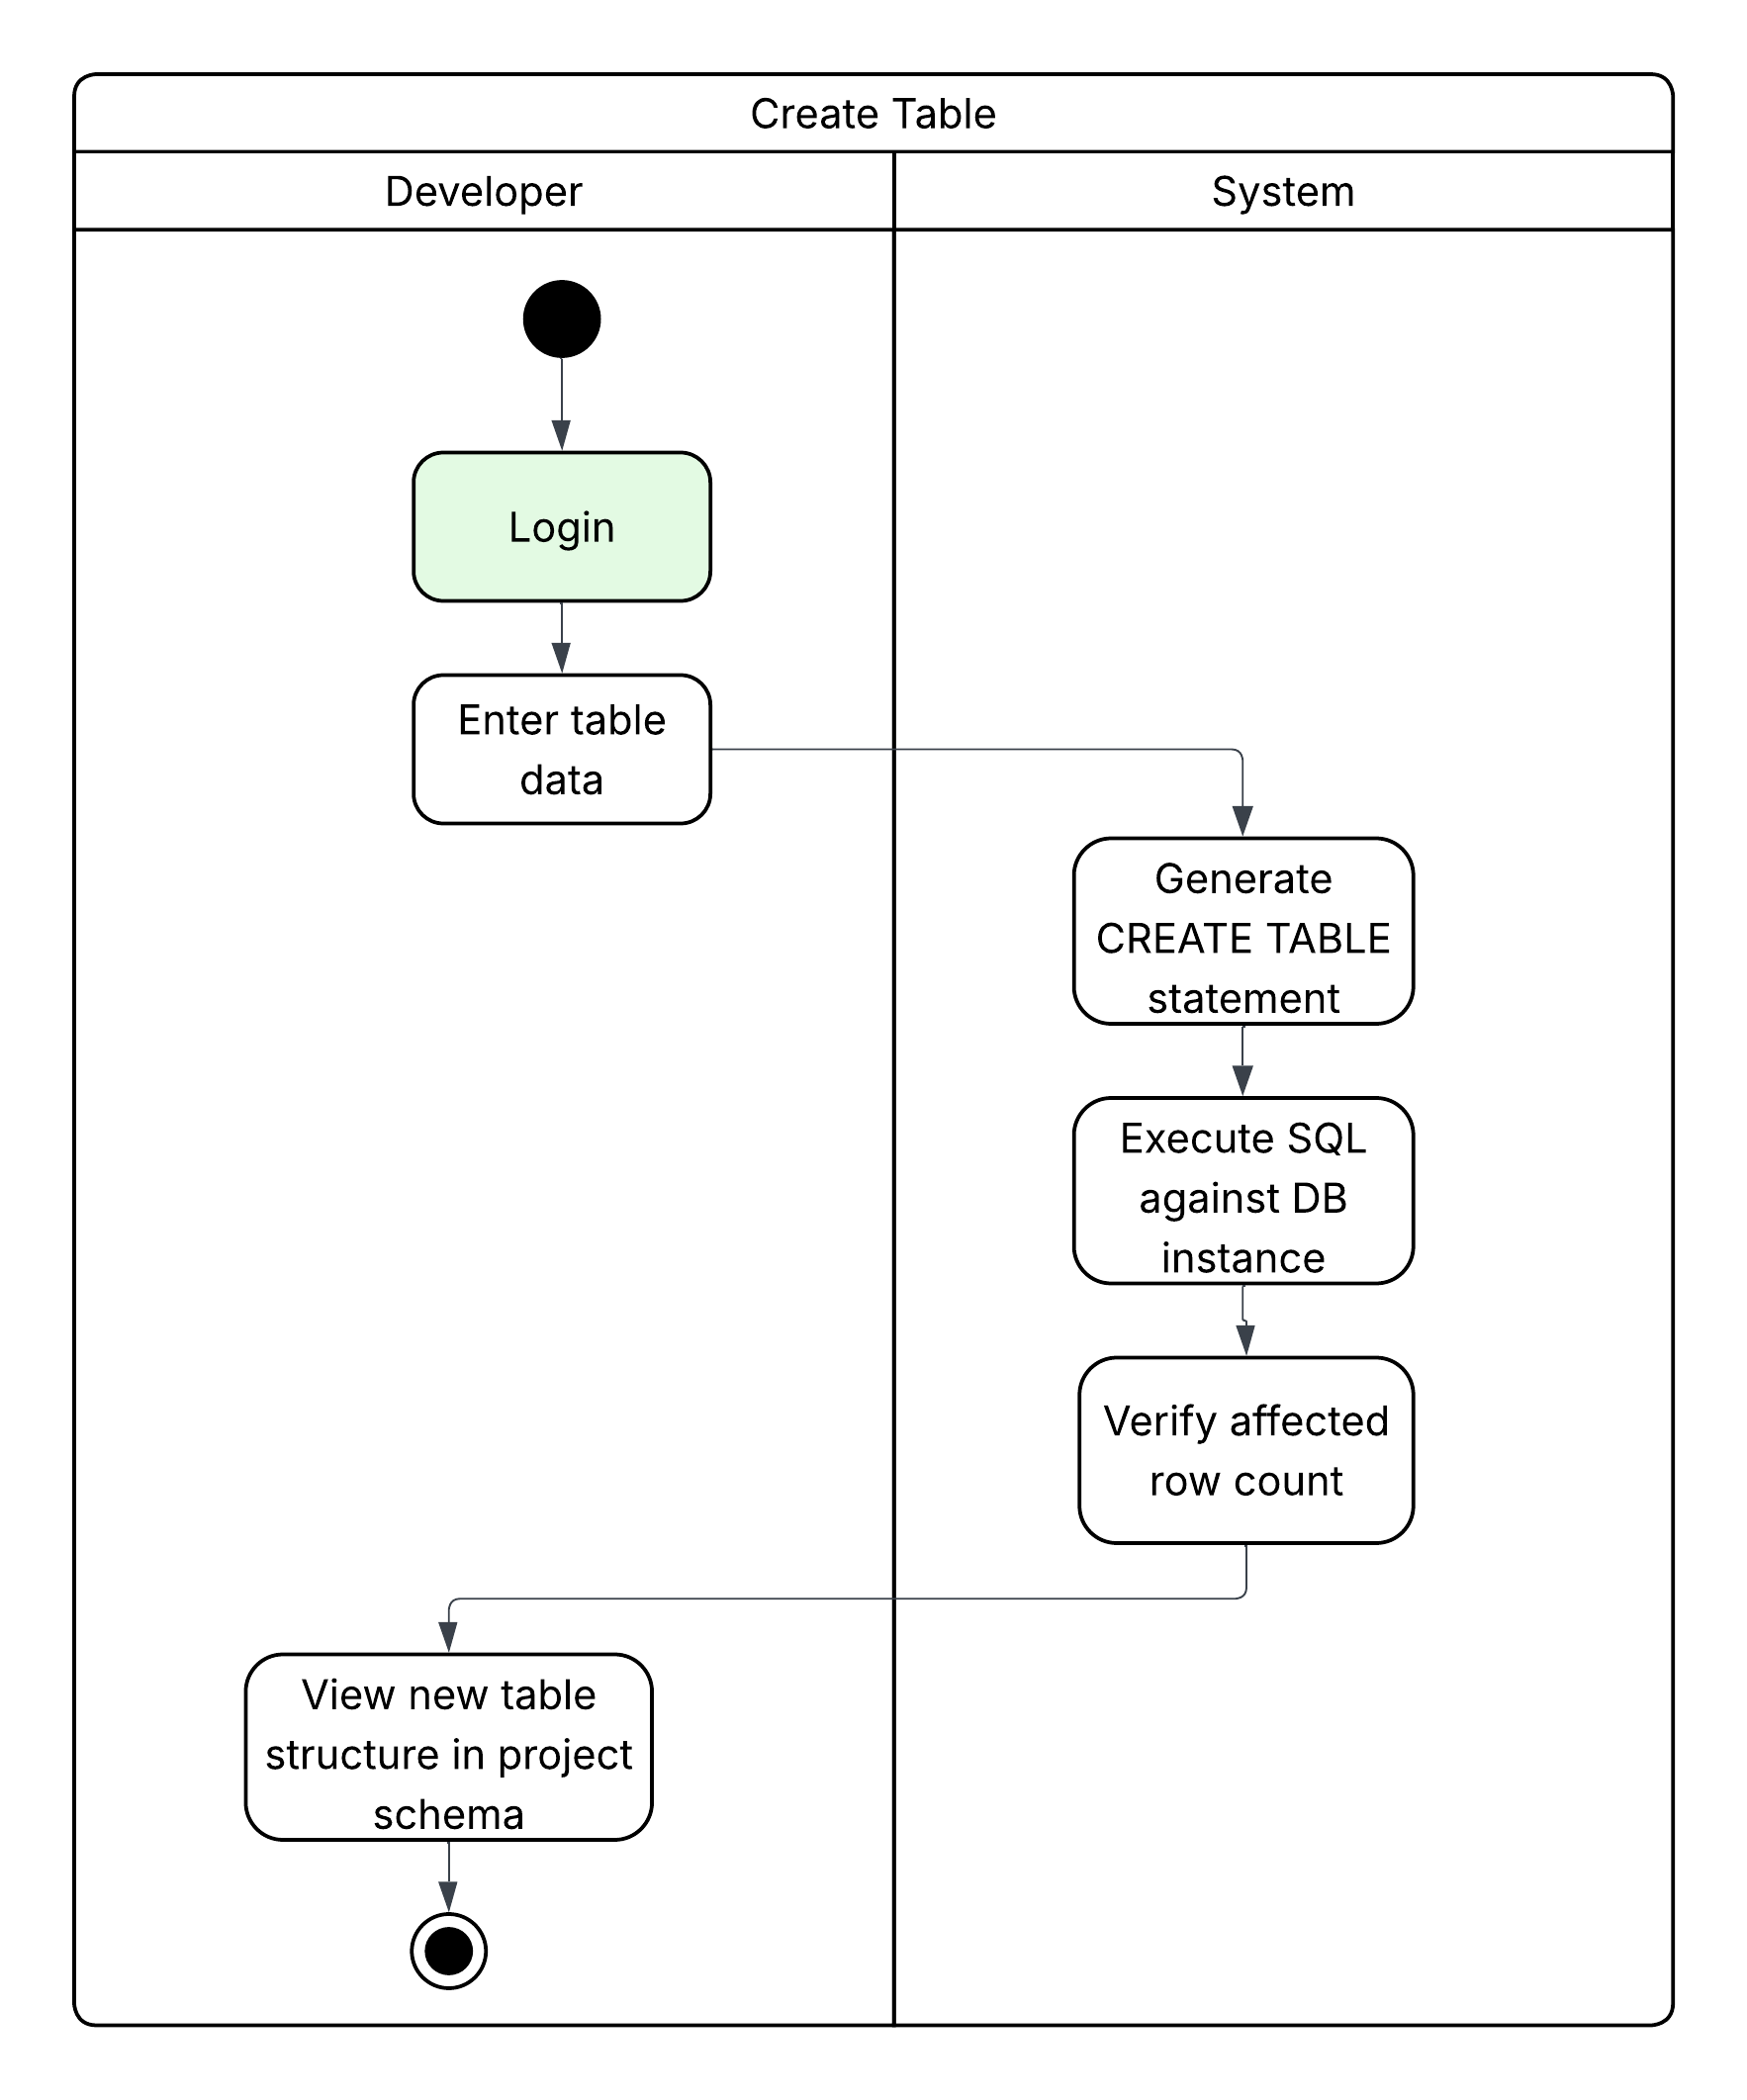
\includegraphics{images/activity/4.Create_Table.png}
        \caption{Create SQL table activity diagram}
        \label{fig:create_table_activity}
    \end{figure}

    \begin{figure}[H]
        \centering
        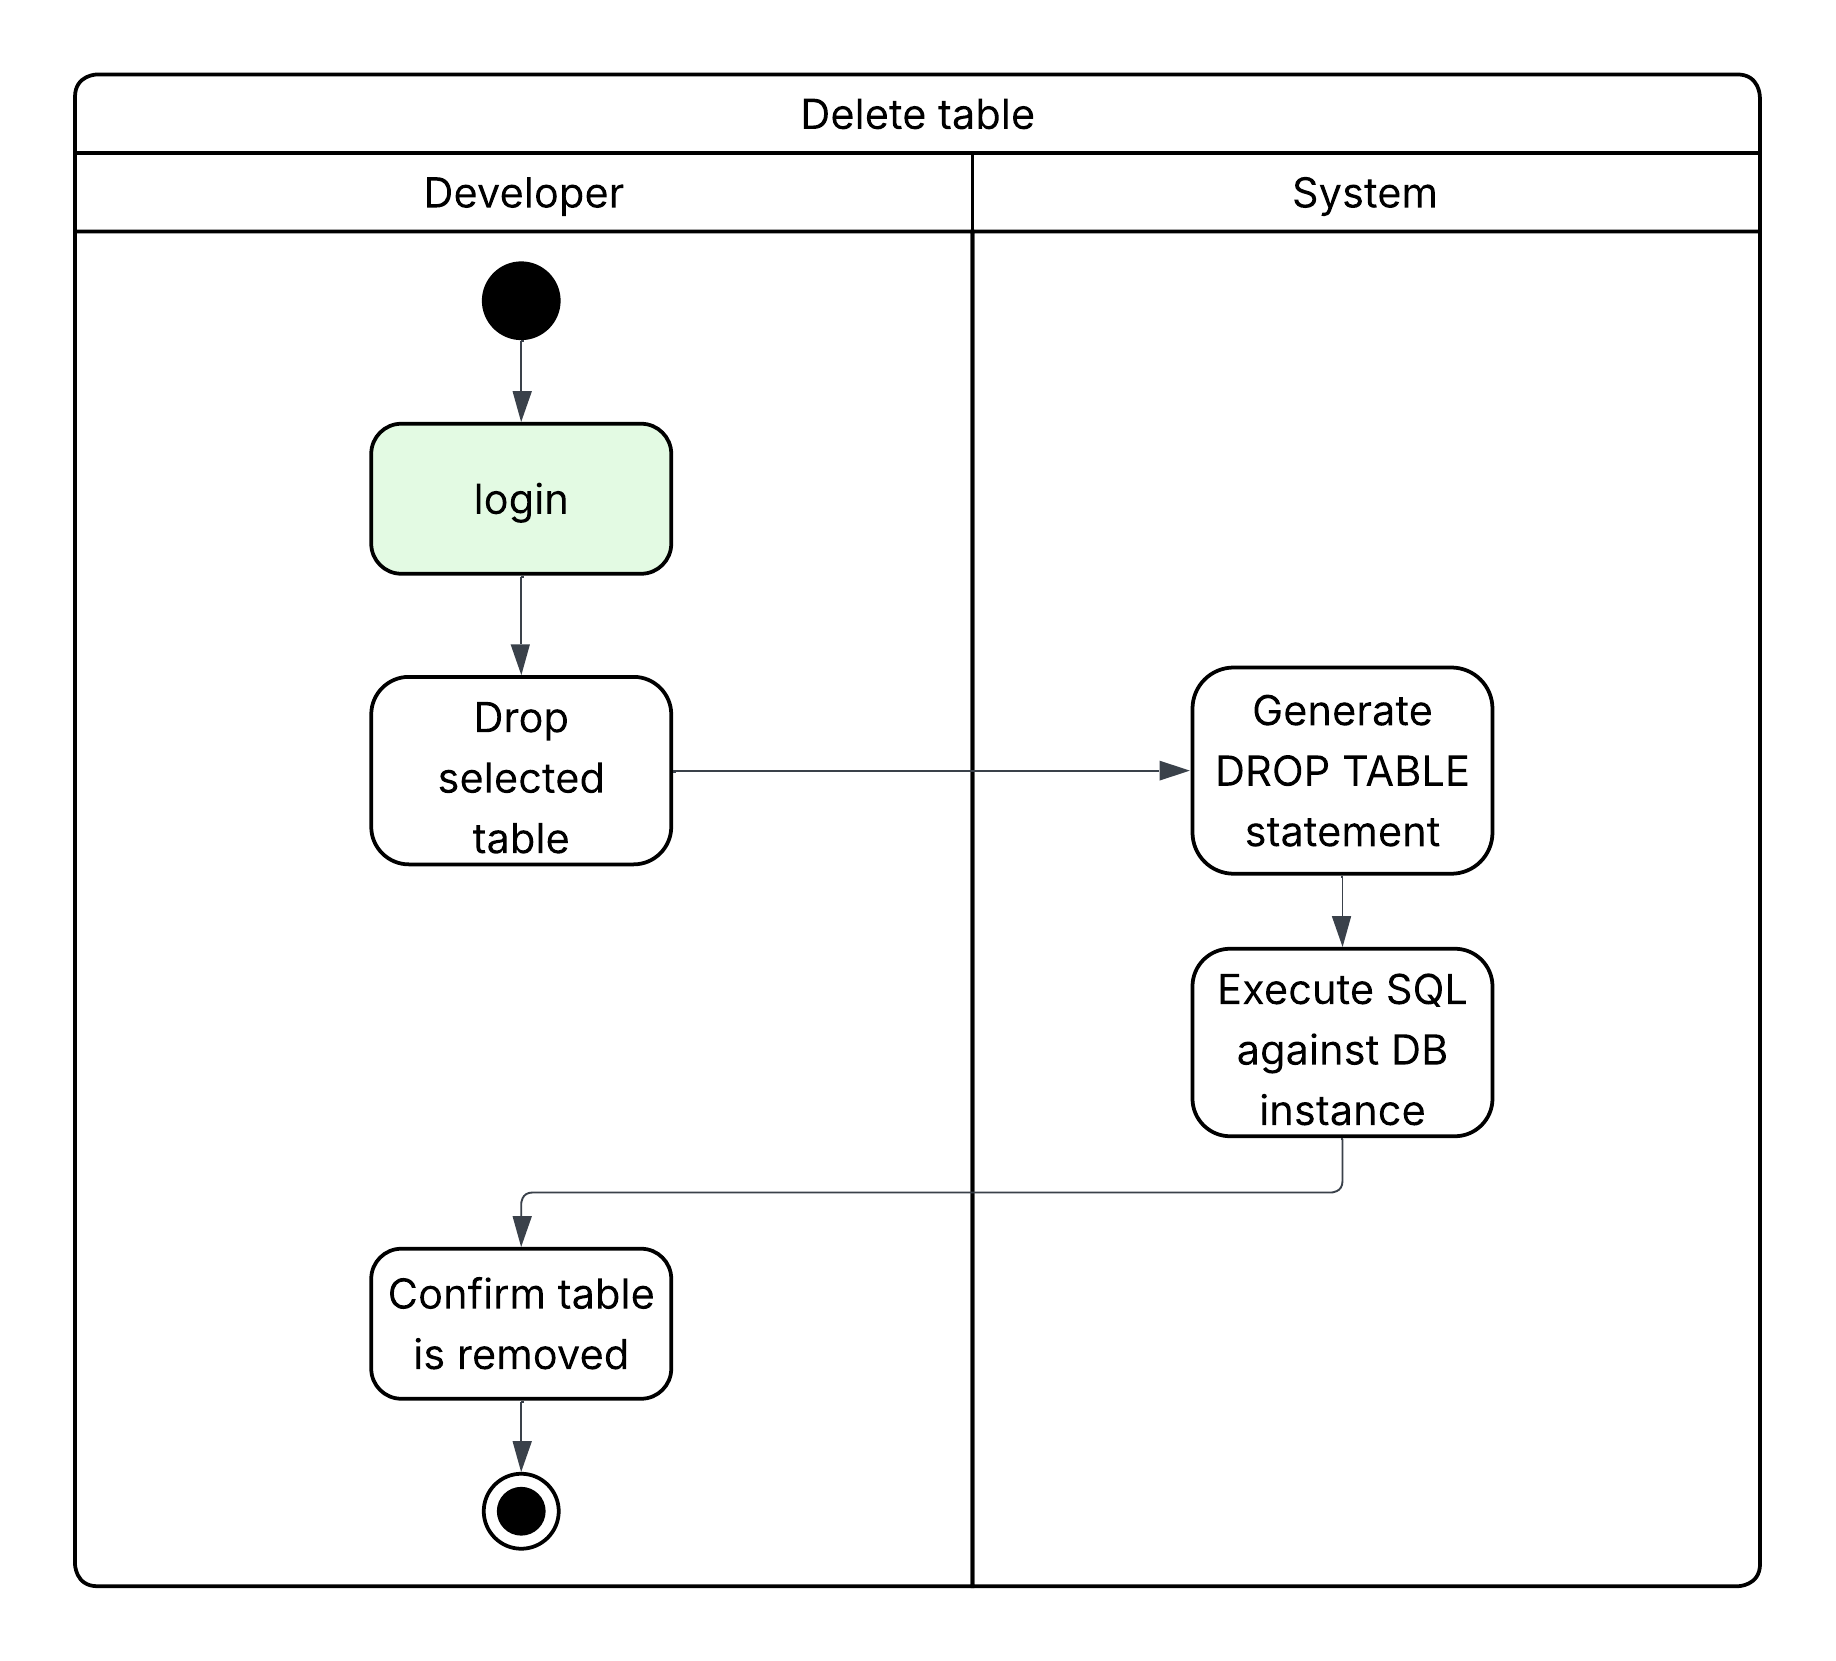
\includegraphics{images/activity/5.Delete_table.png}
        \caption{Delete SQL table activity diagram}
        \label{fig:delete_table_activity}
    \end{figure}

    % \begin{figure}[H]
    %     \centering
    %     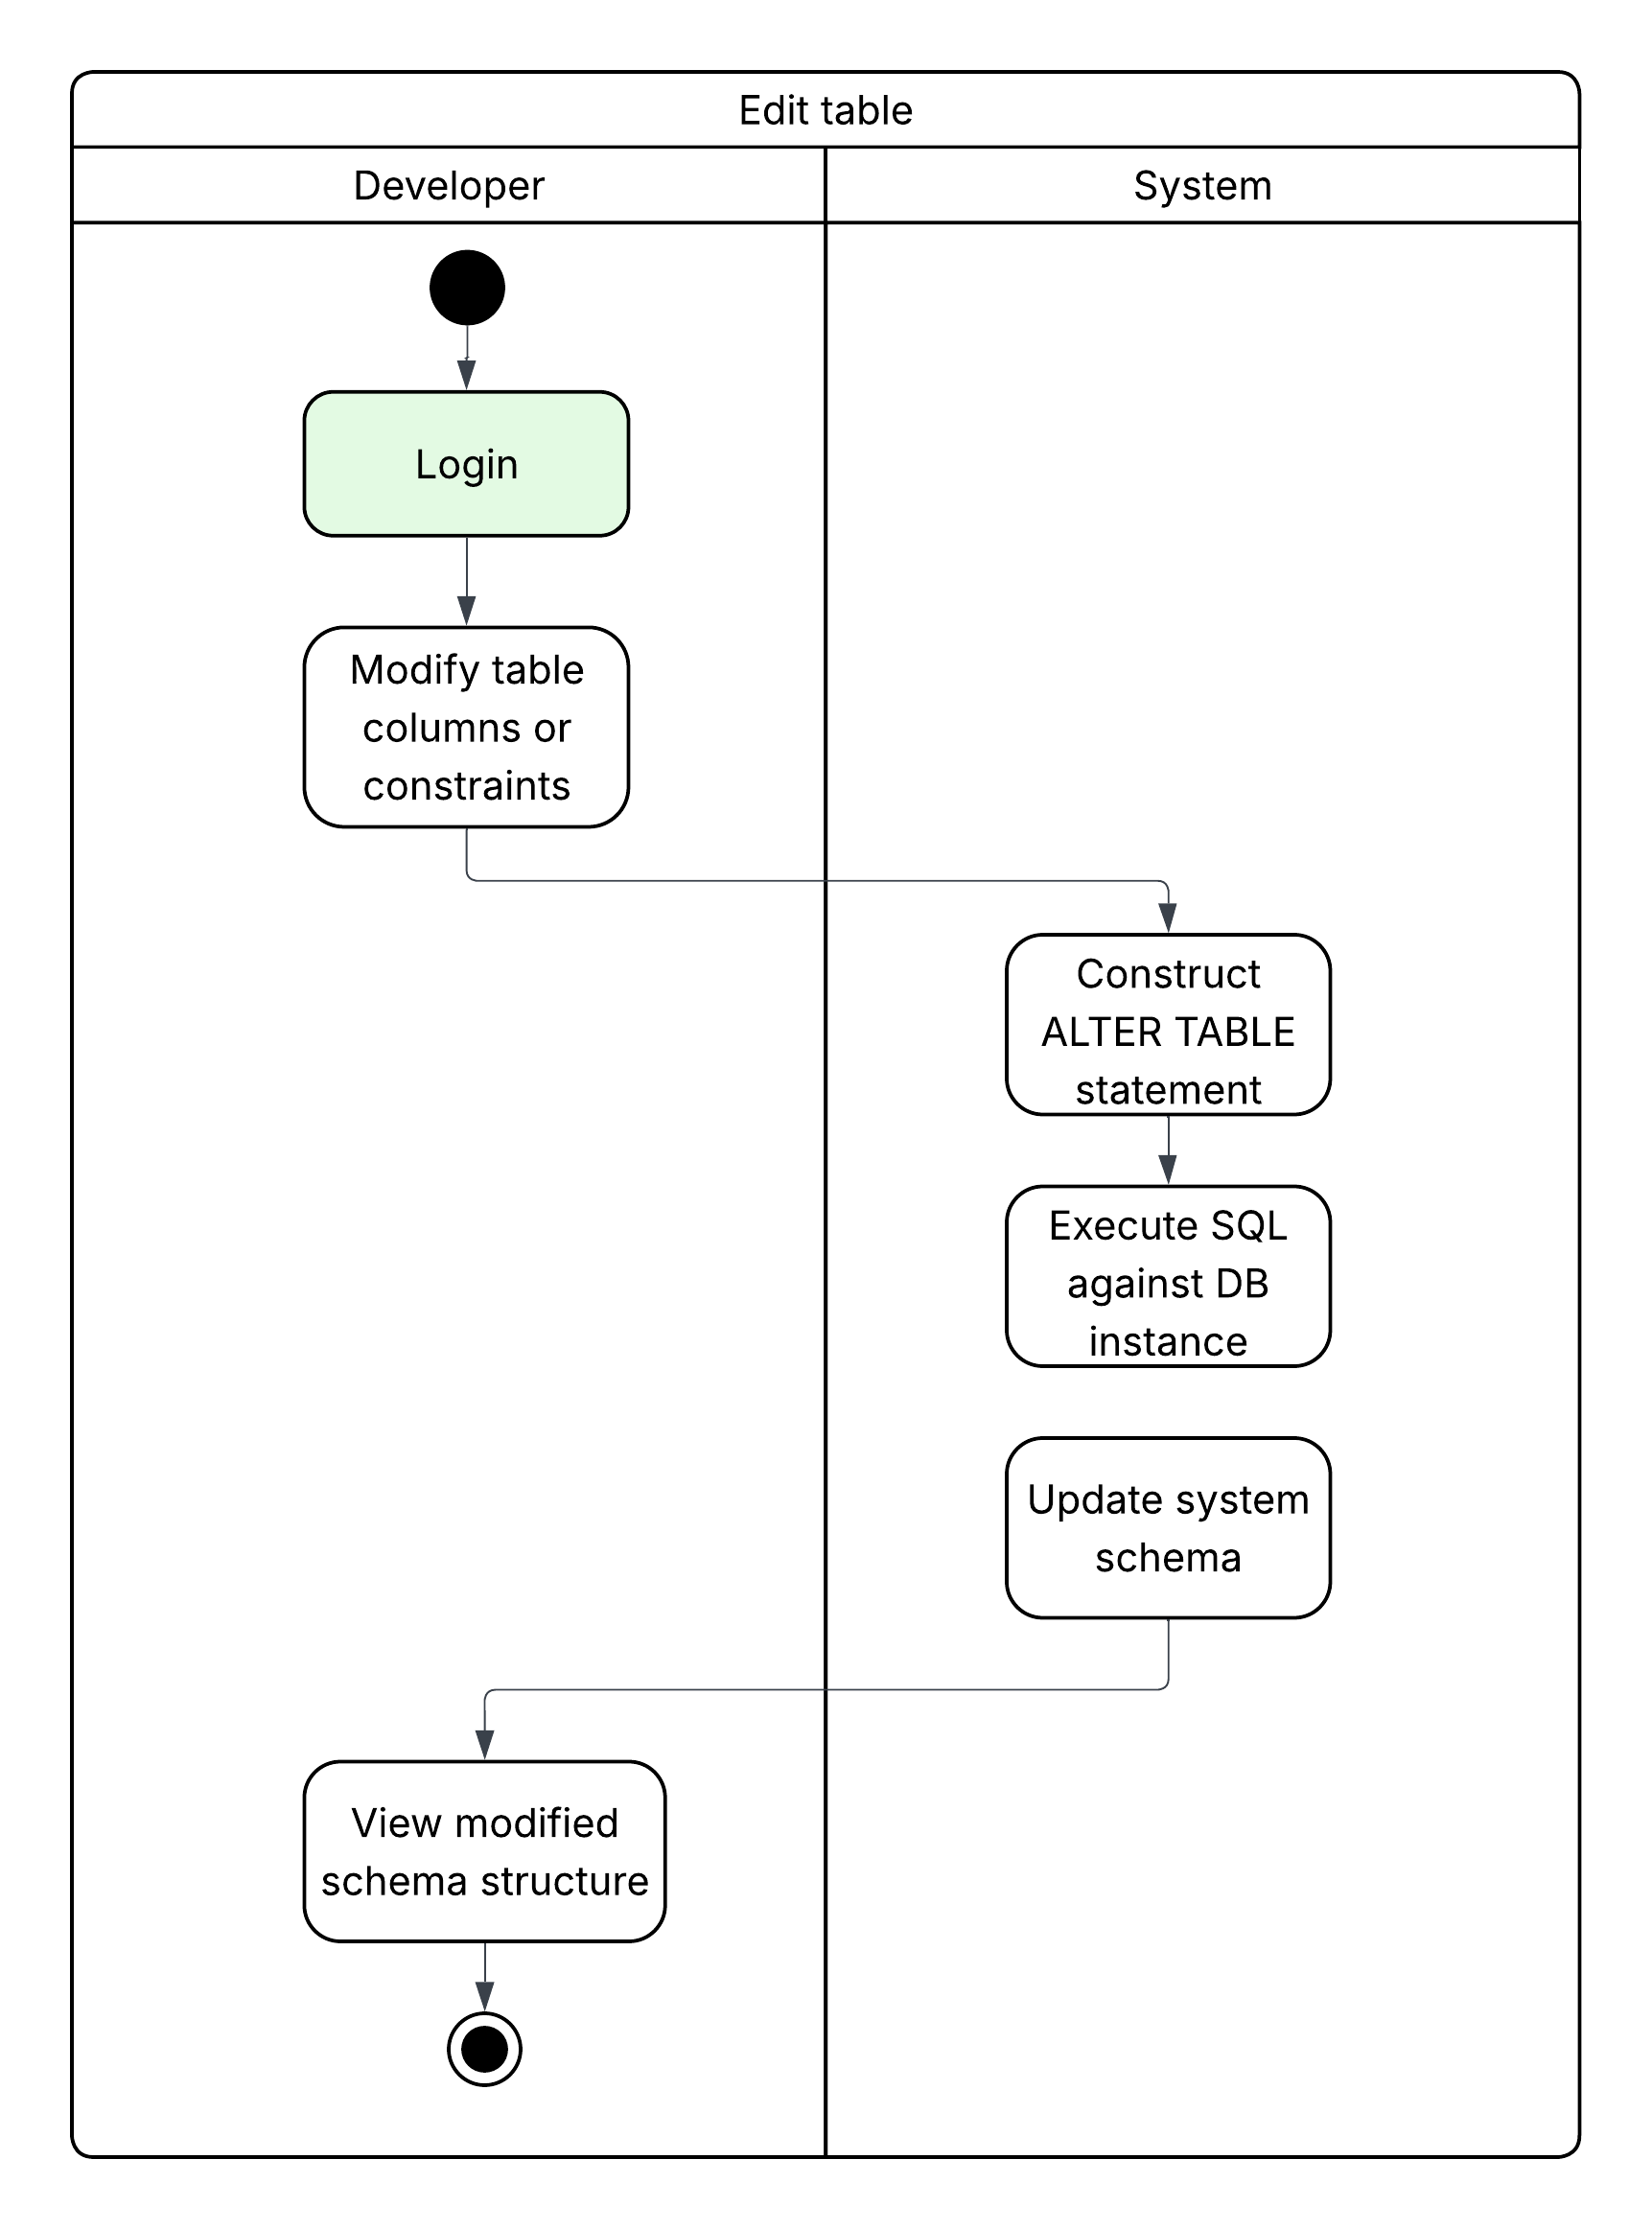
\includegraphics{images/activity/6.Edit_Table.png}
    %     \caption{Edit SQL table activity diagram}
    %     \label{fig:edit_table_activity}
    % \end{figure}

    \begin{figure}[H]
        \centering
        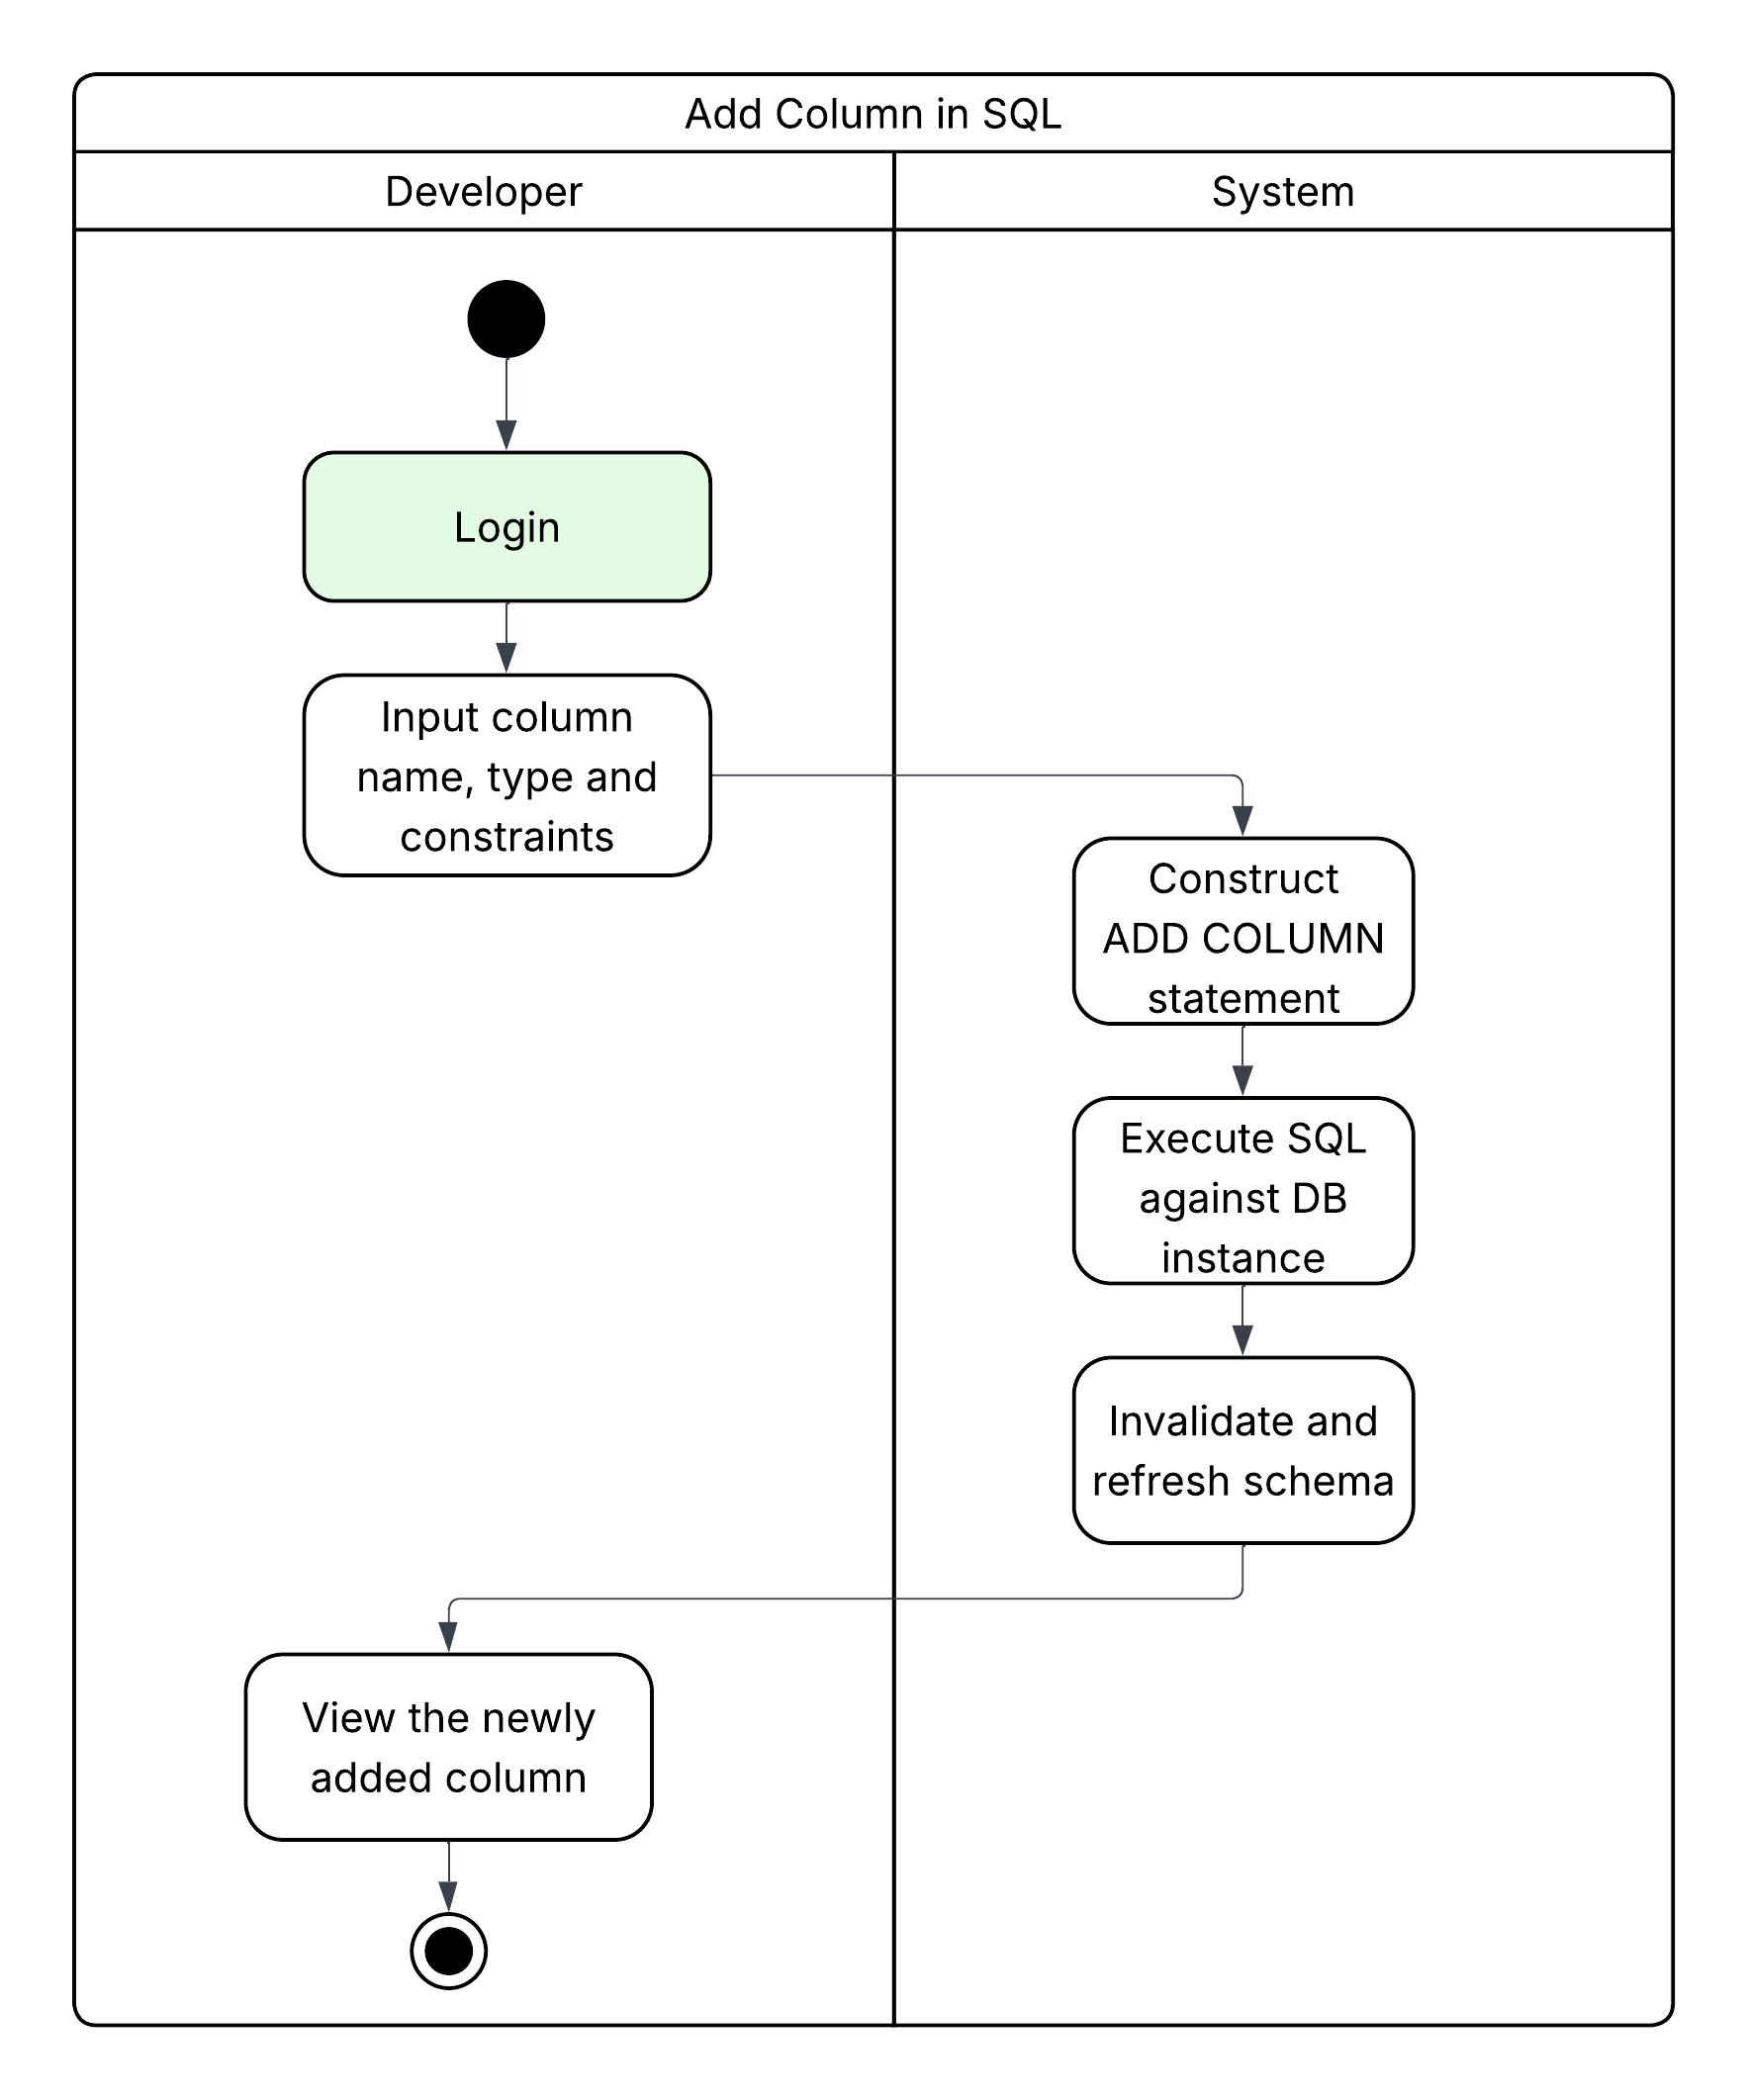
\includegraphics{images/activity/19.Add_Column.png}
        \caption{Add SQL column activity diagram}
        \label{fig:Add_Column}
    \end{figure}

    \begin{figure}[H]
        \centering
        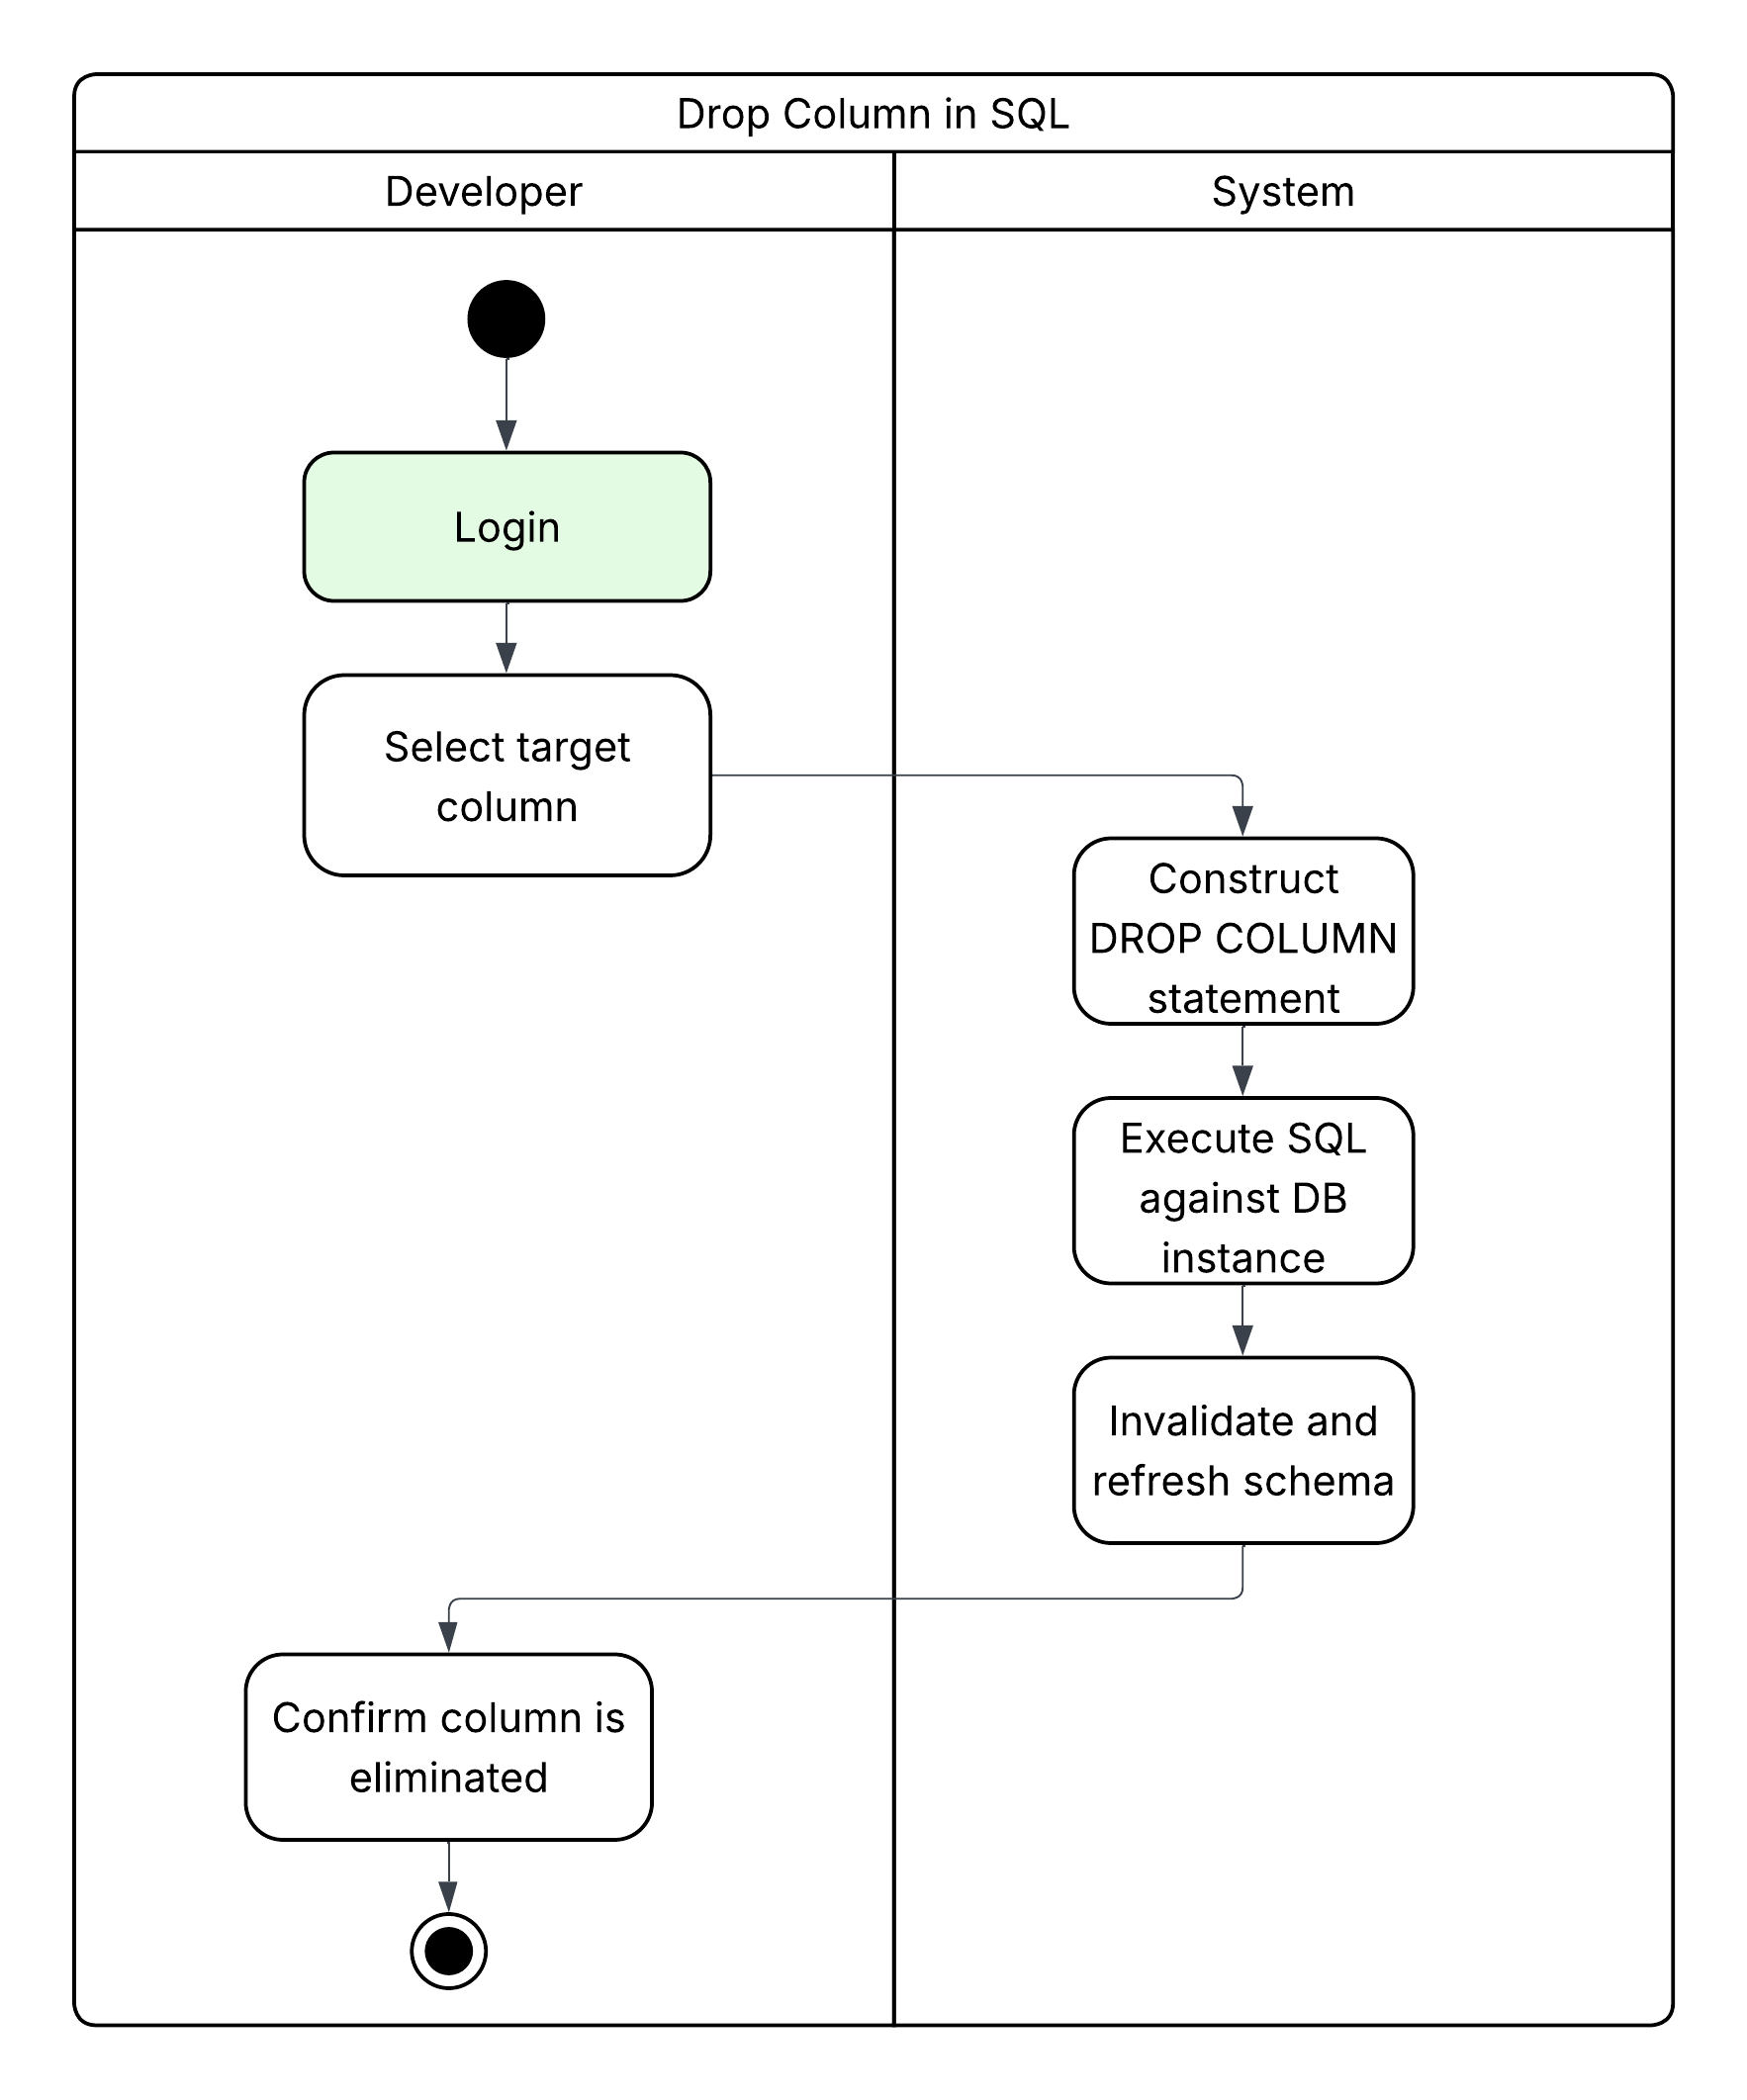
\includegraphics{images/activity/20.Drop_Column.png}
        \caption{Drop SQL column activity diagram}
        \label{fig:Drop_Column}
    \end{figure}

    \begin{figure}[H]
        \centering
        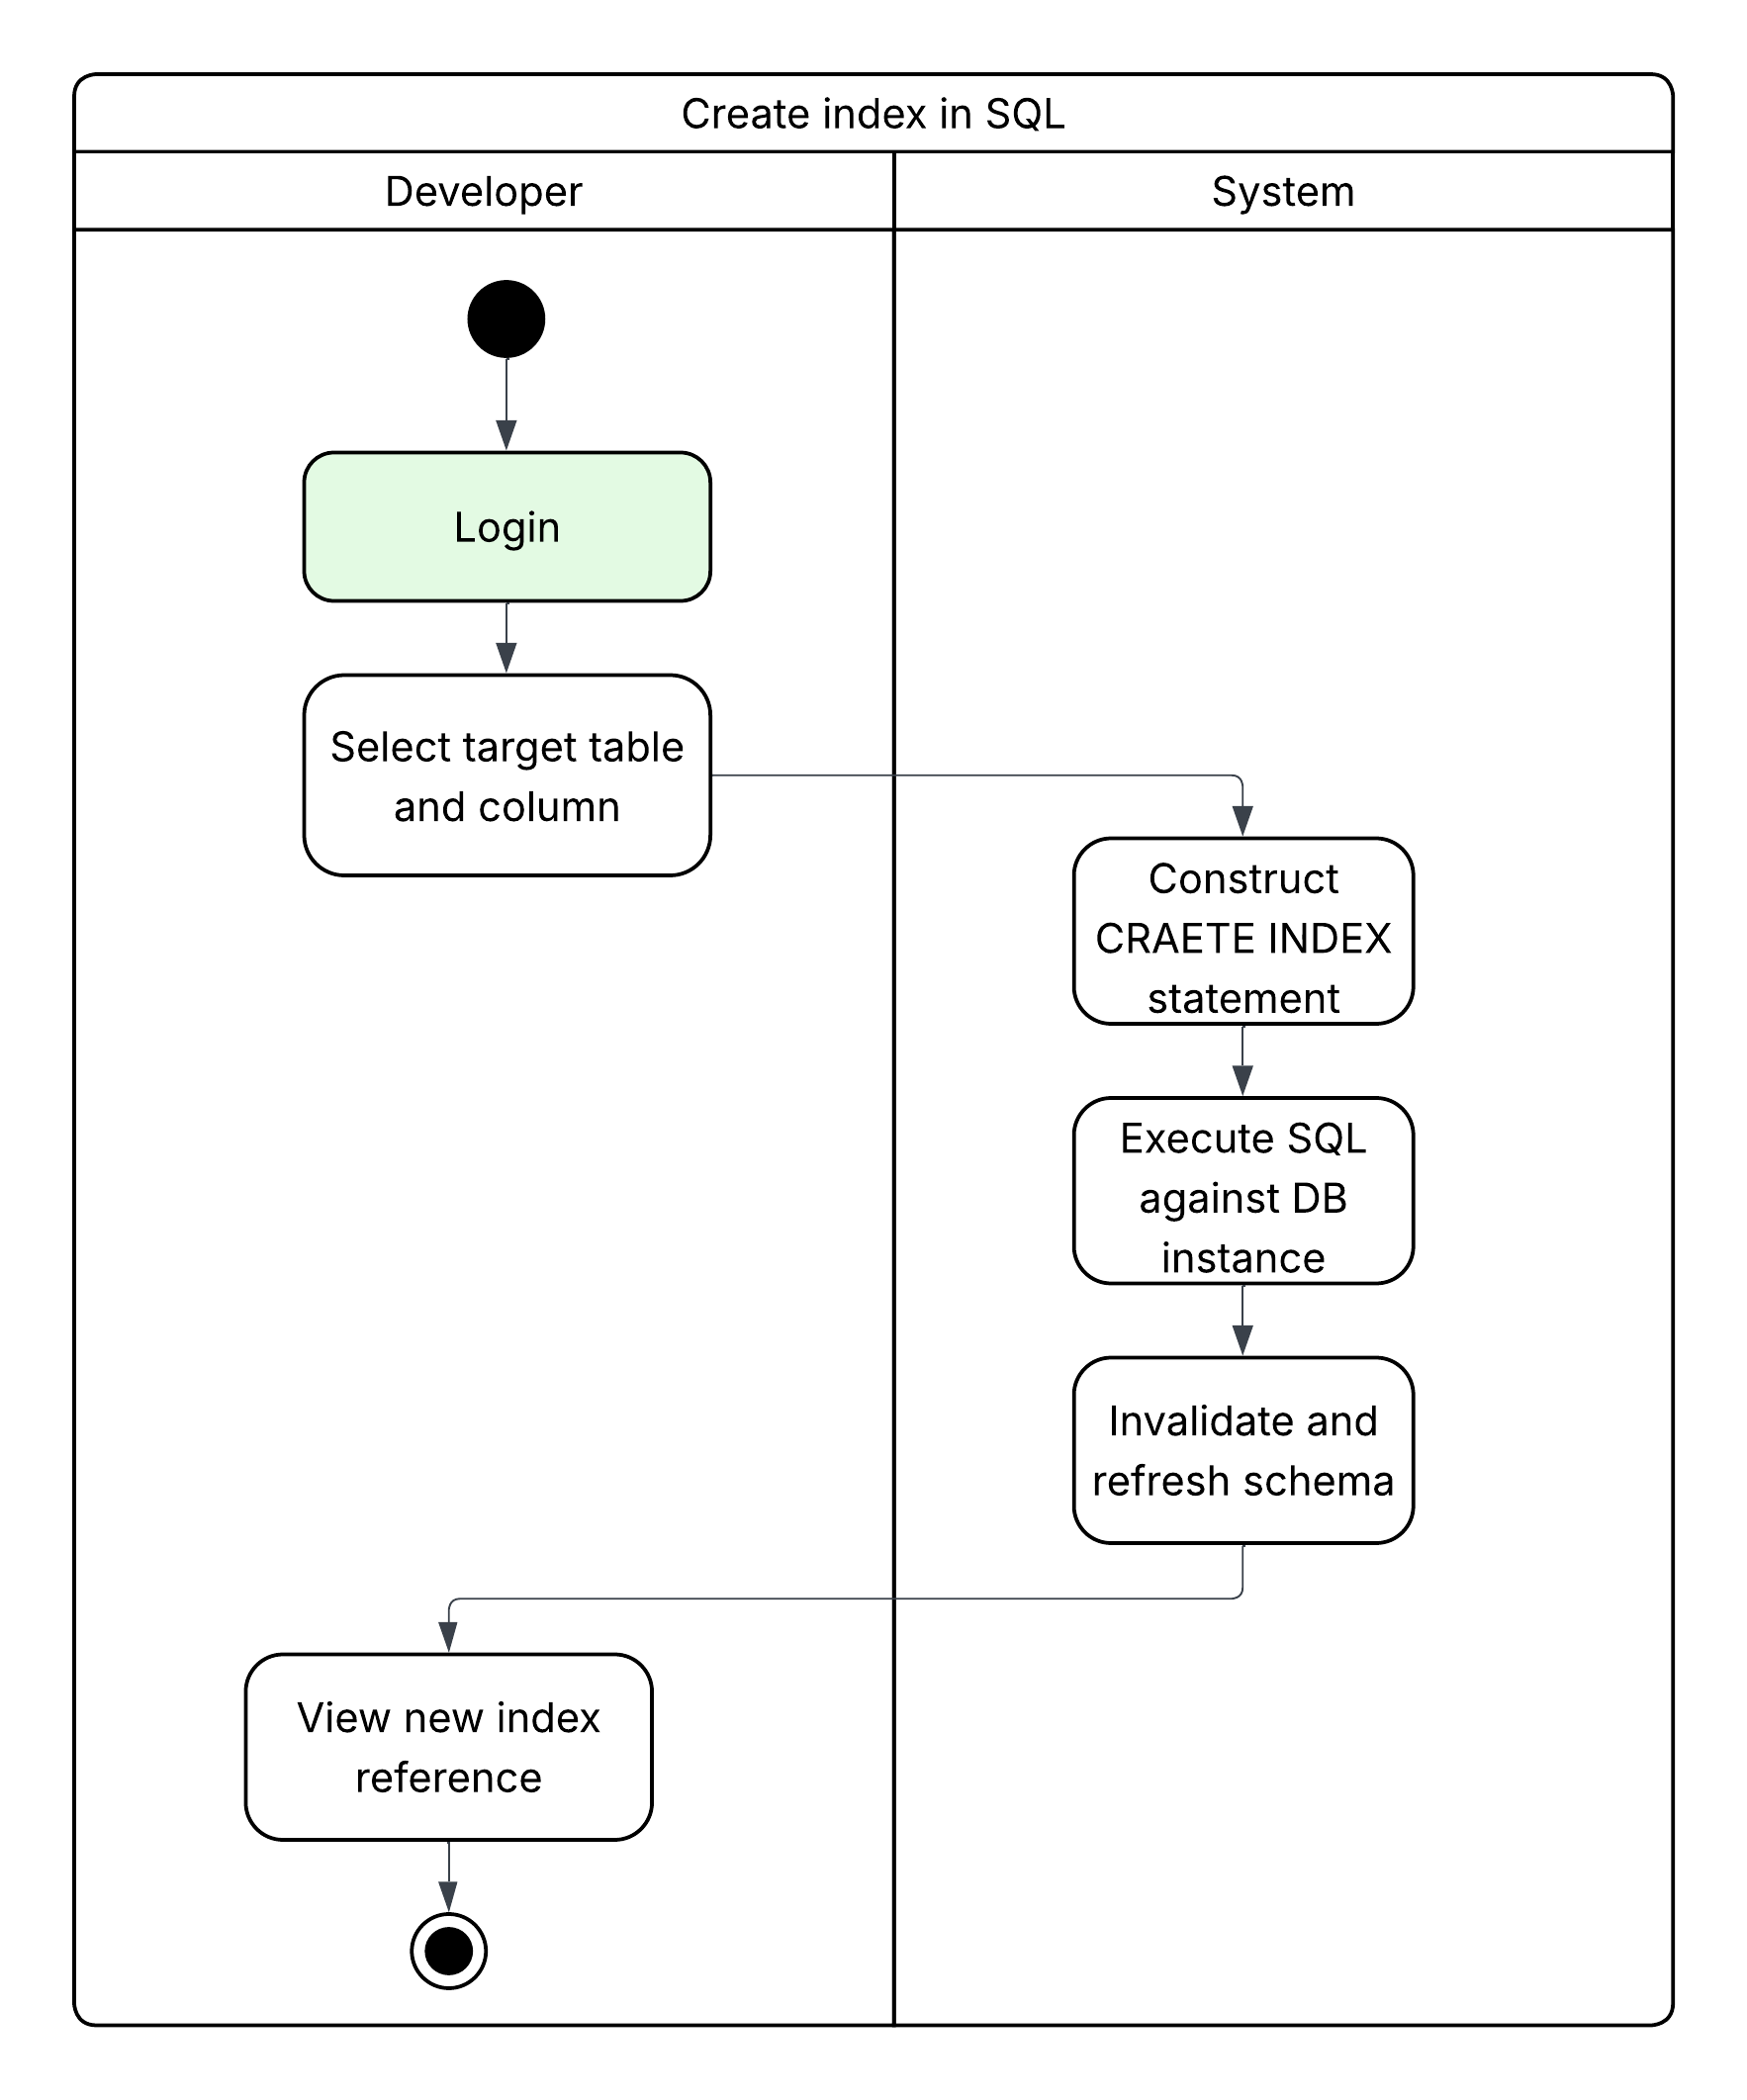
\includegraphics{images/activity/21.Create_Index.png}
        \caption{Create SQL index activity diagram}
        \label{fig:Create_Index}
    \end{figure}

    \begin{figure}[H]
        \centering
        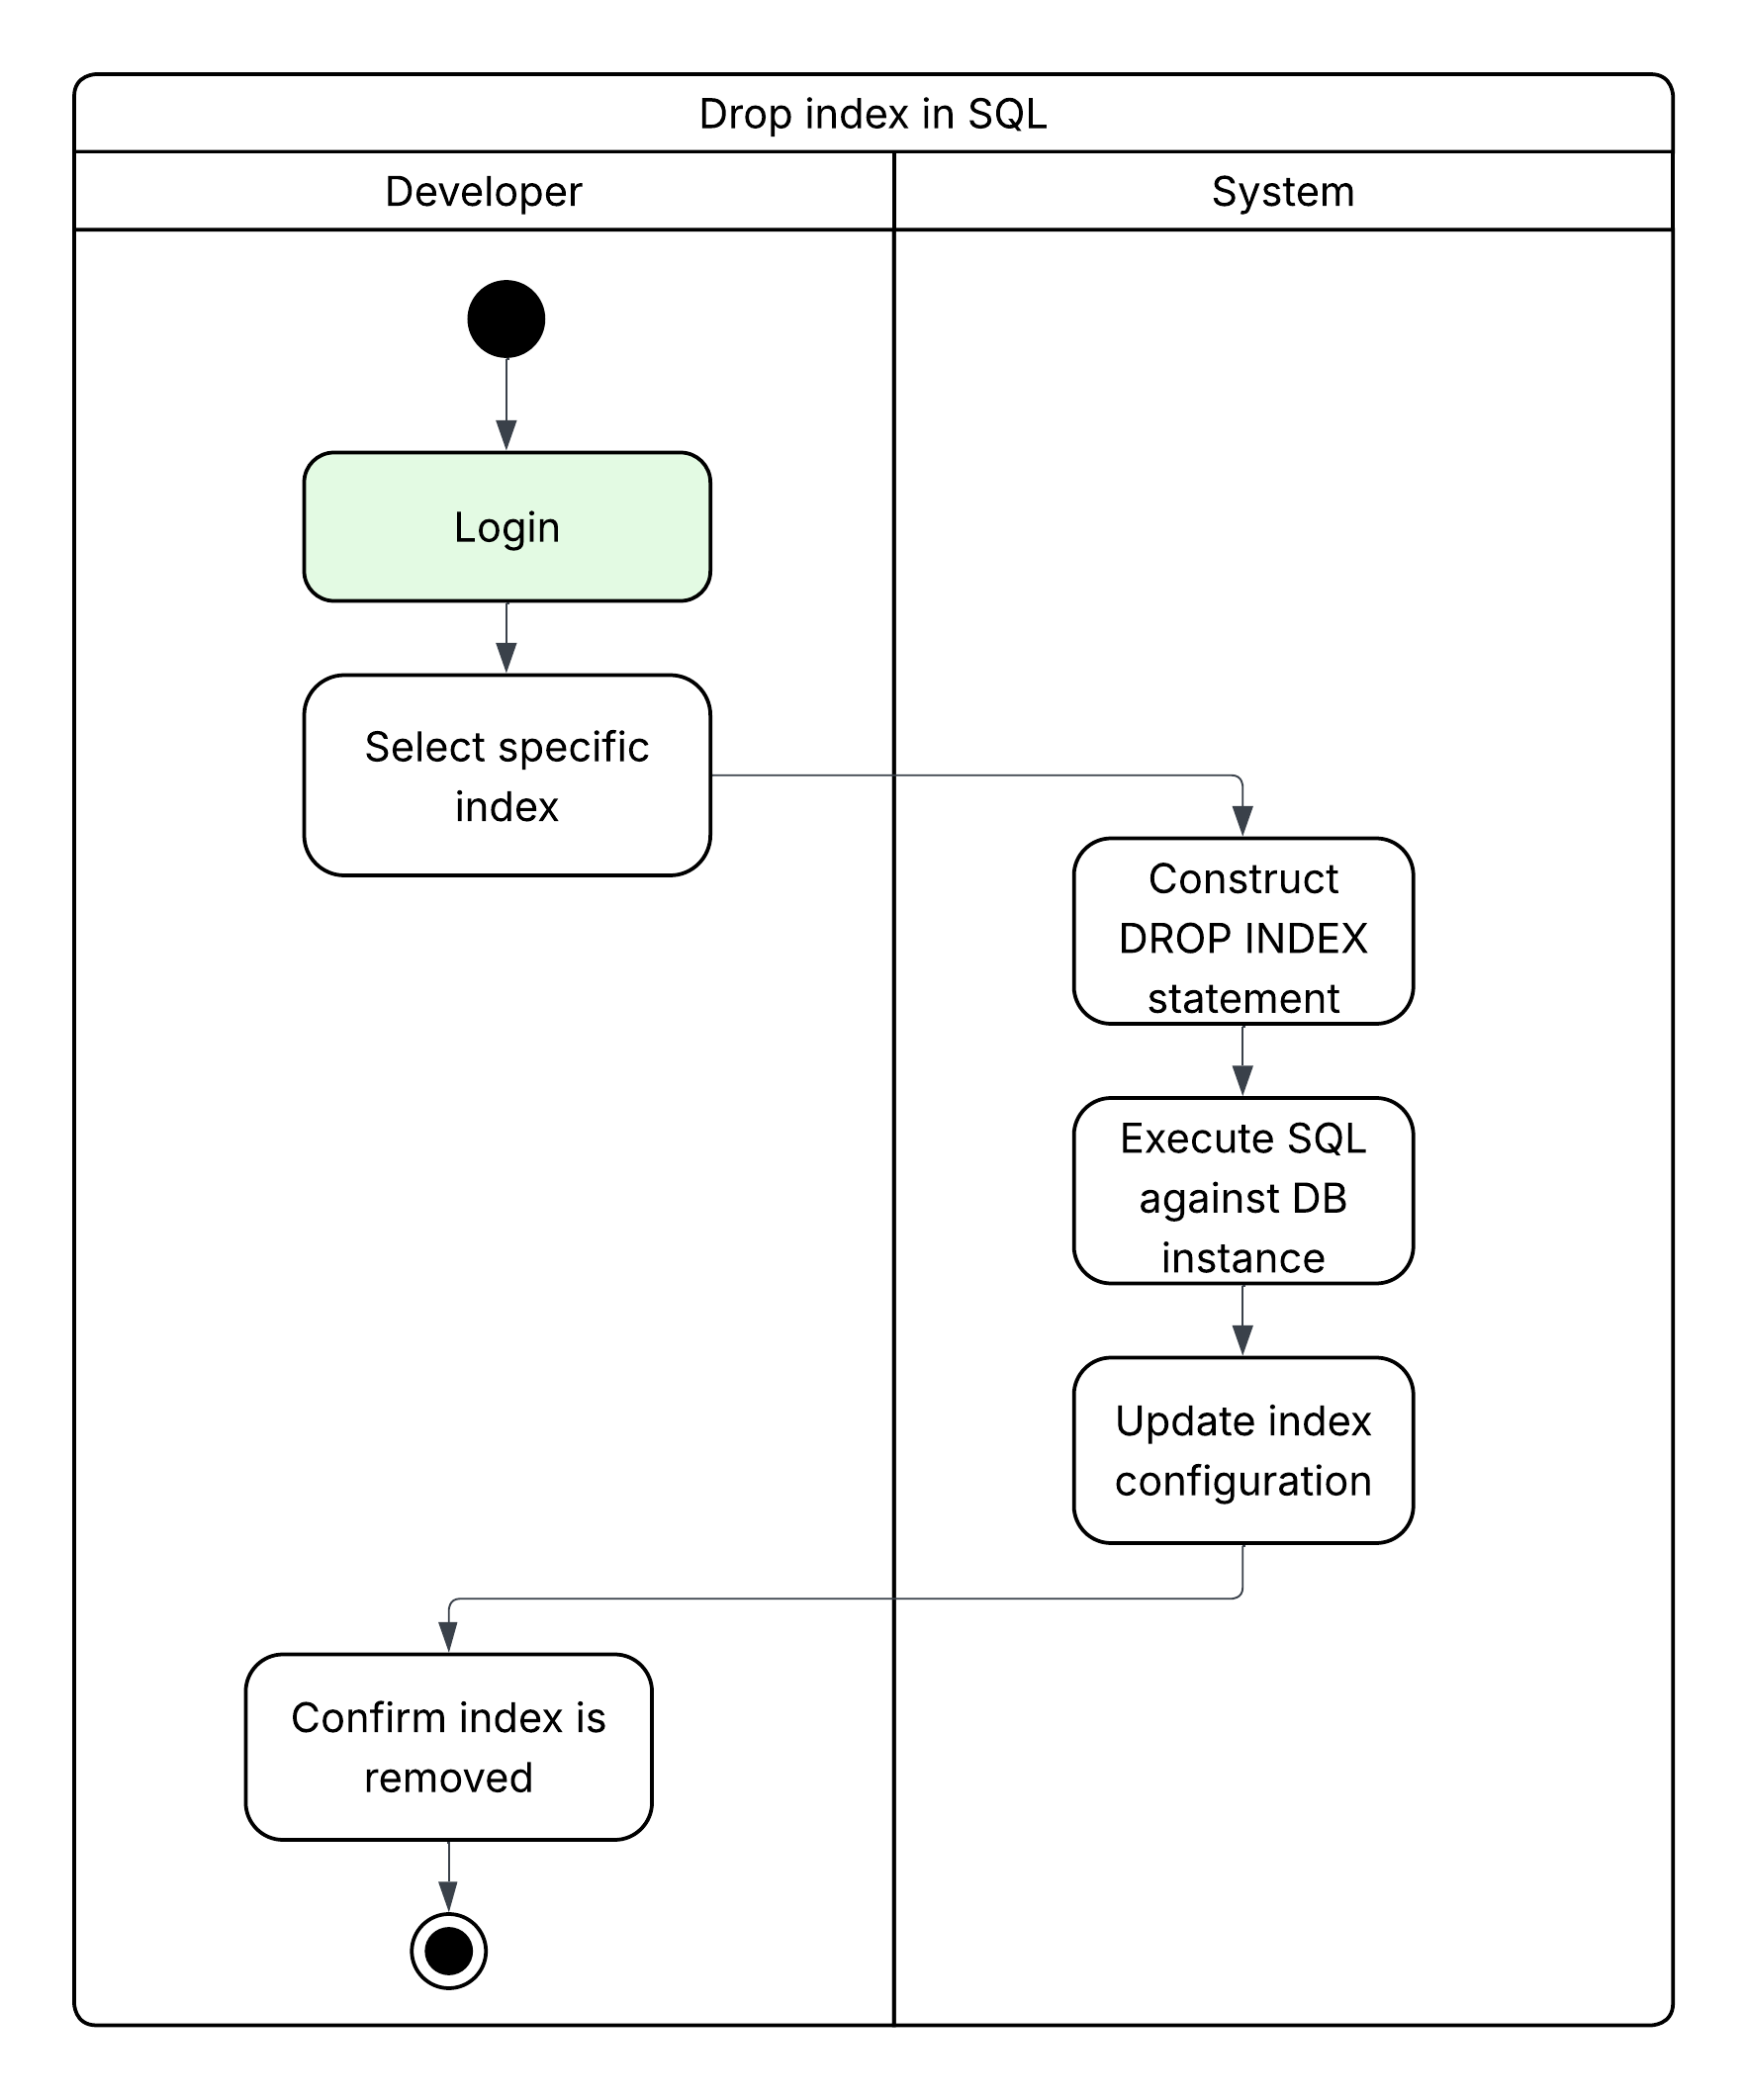
\includegraphics{images/activity/22.Drop_Index.png}
        \caption{Drop SQL index activity diagram}
        \label{fig:Drop_Index}
    \end{figure}

    \begin{figure}[H]
        \centering
        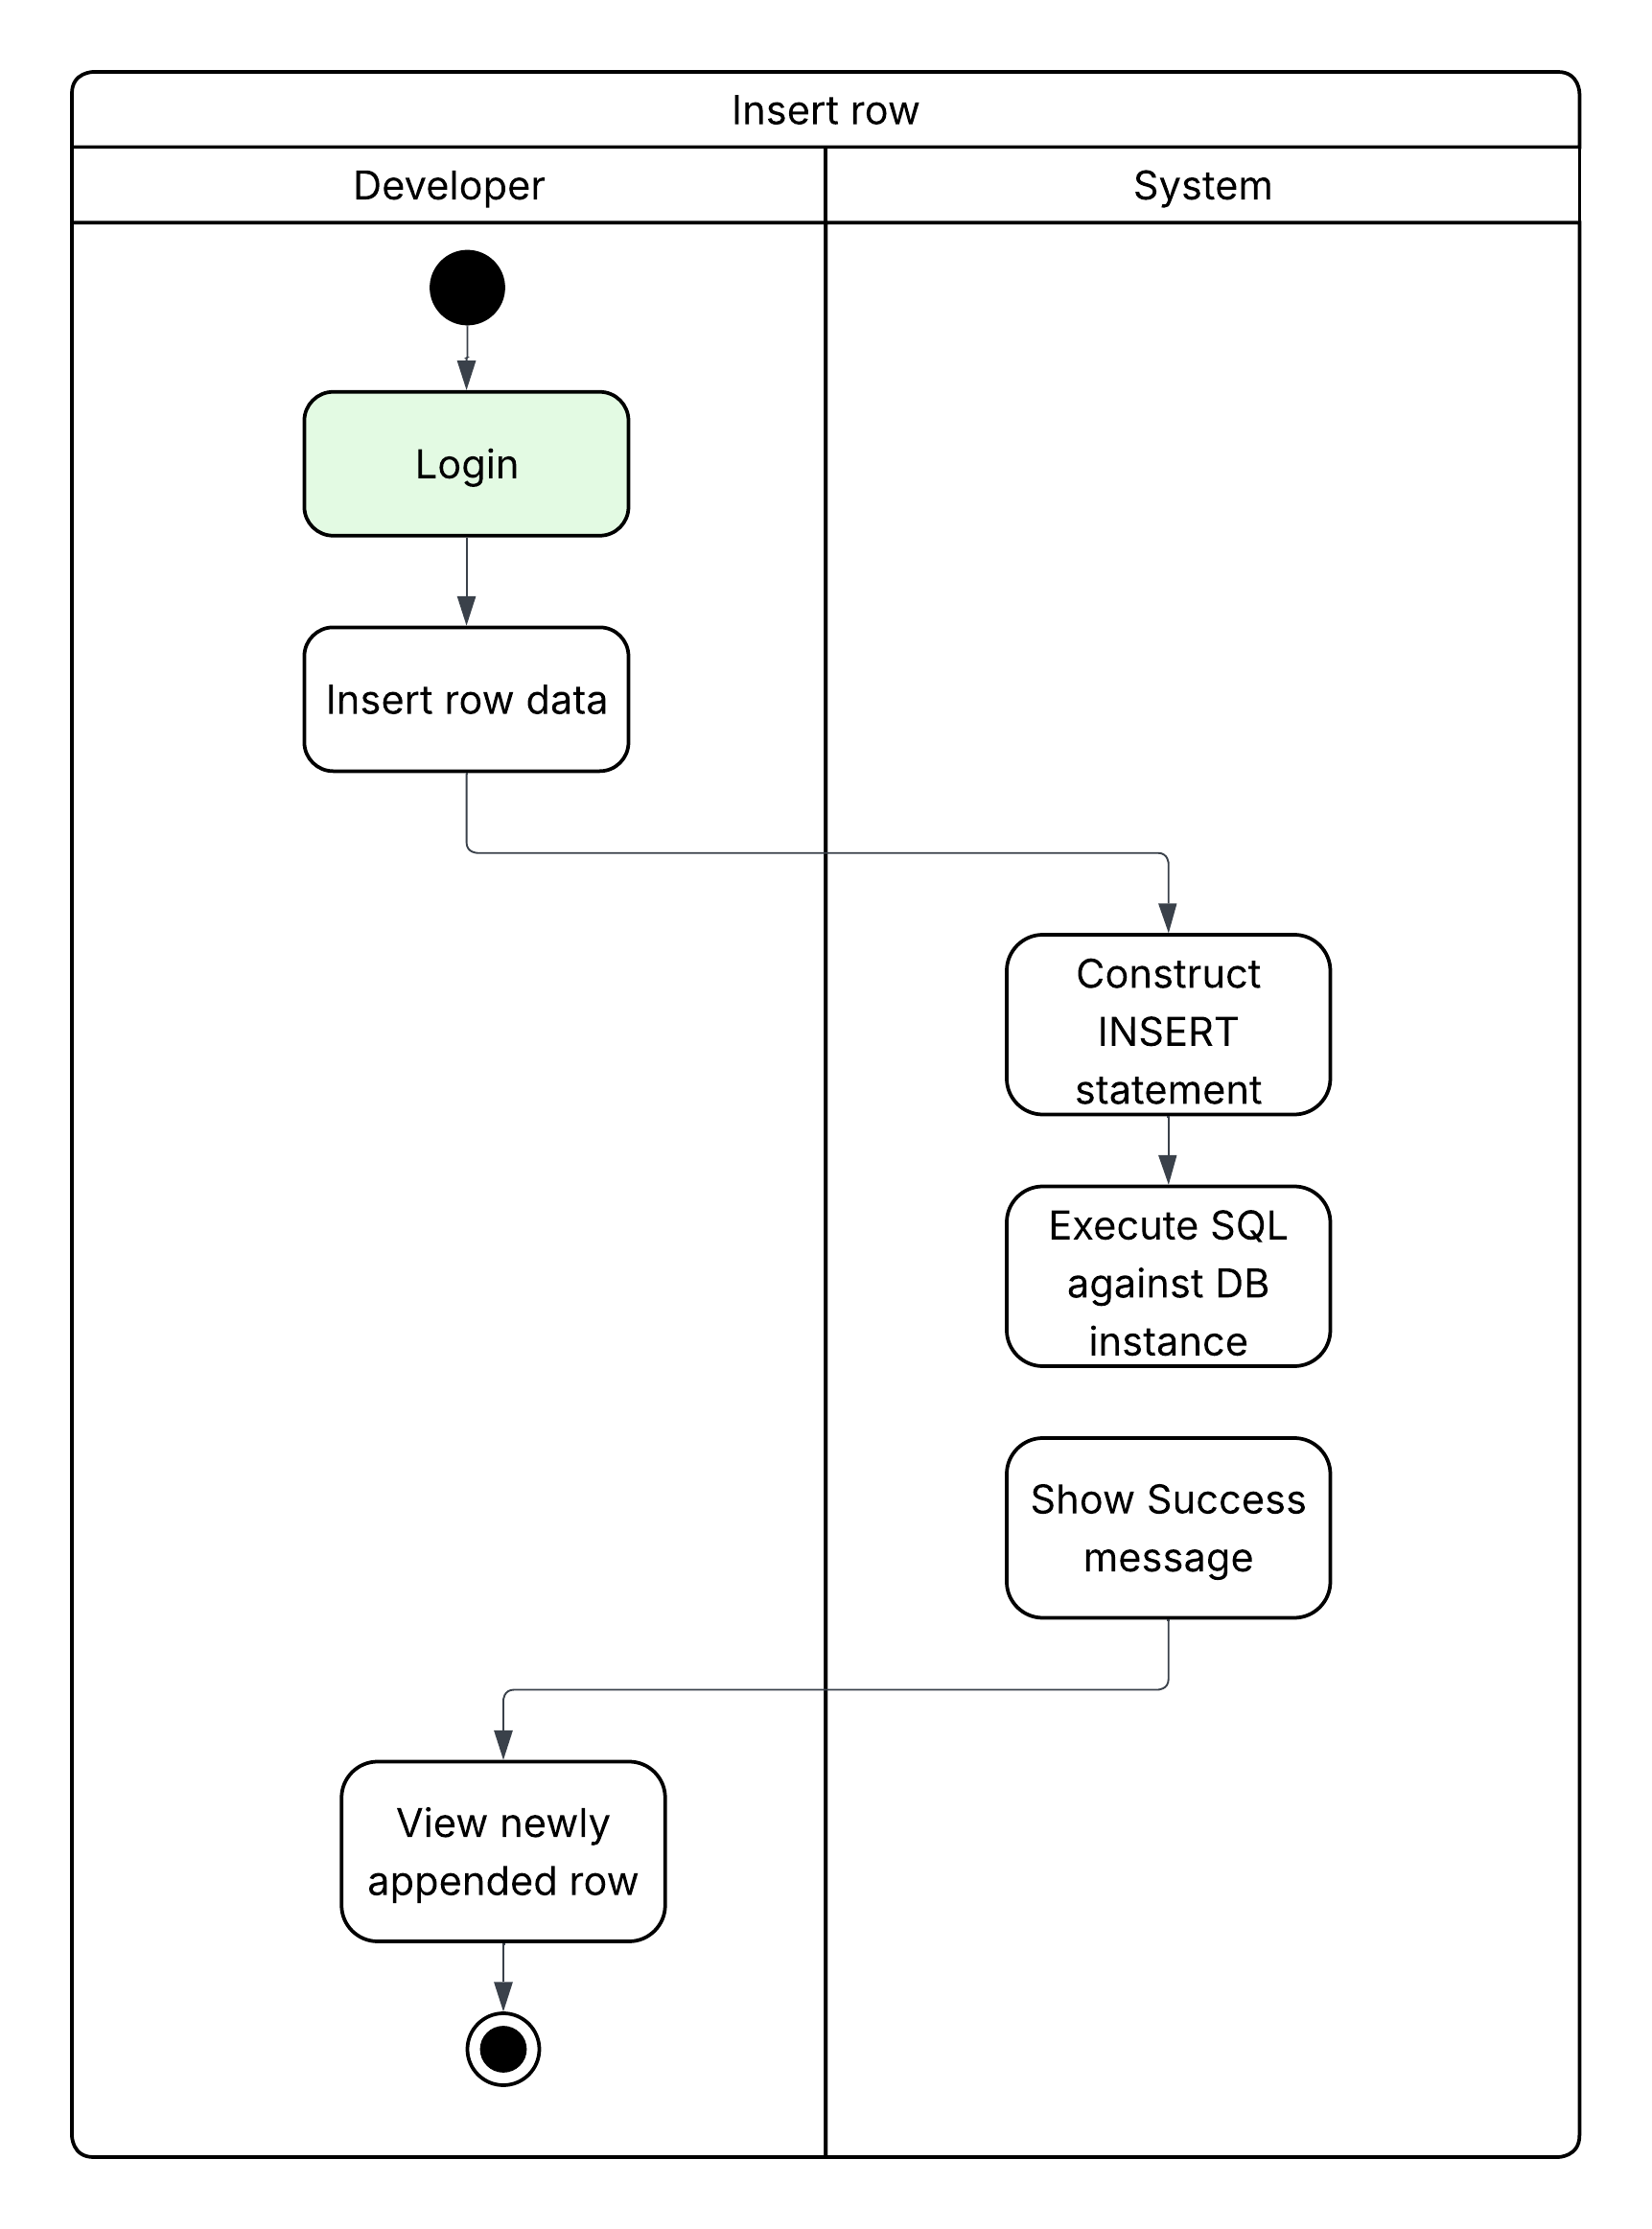
\includegraphics{images/activity/1.Insert_Row.png}
        \caption{Insert SQL rows activity diagram}
        \label{fig:insert_rows_activity}
    \end{figure}
    
    \begin{figure}[H]
        \centering
        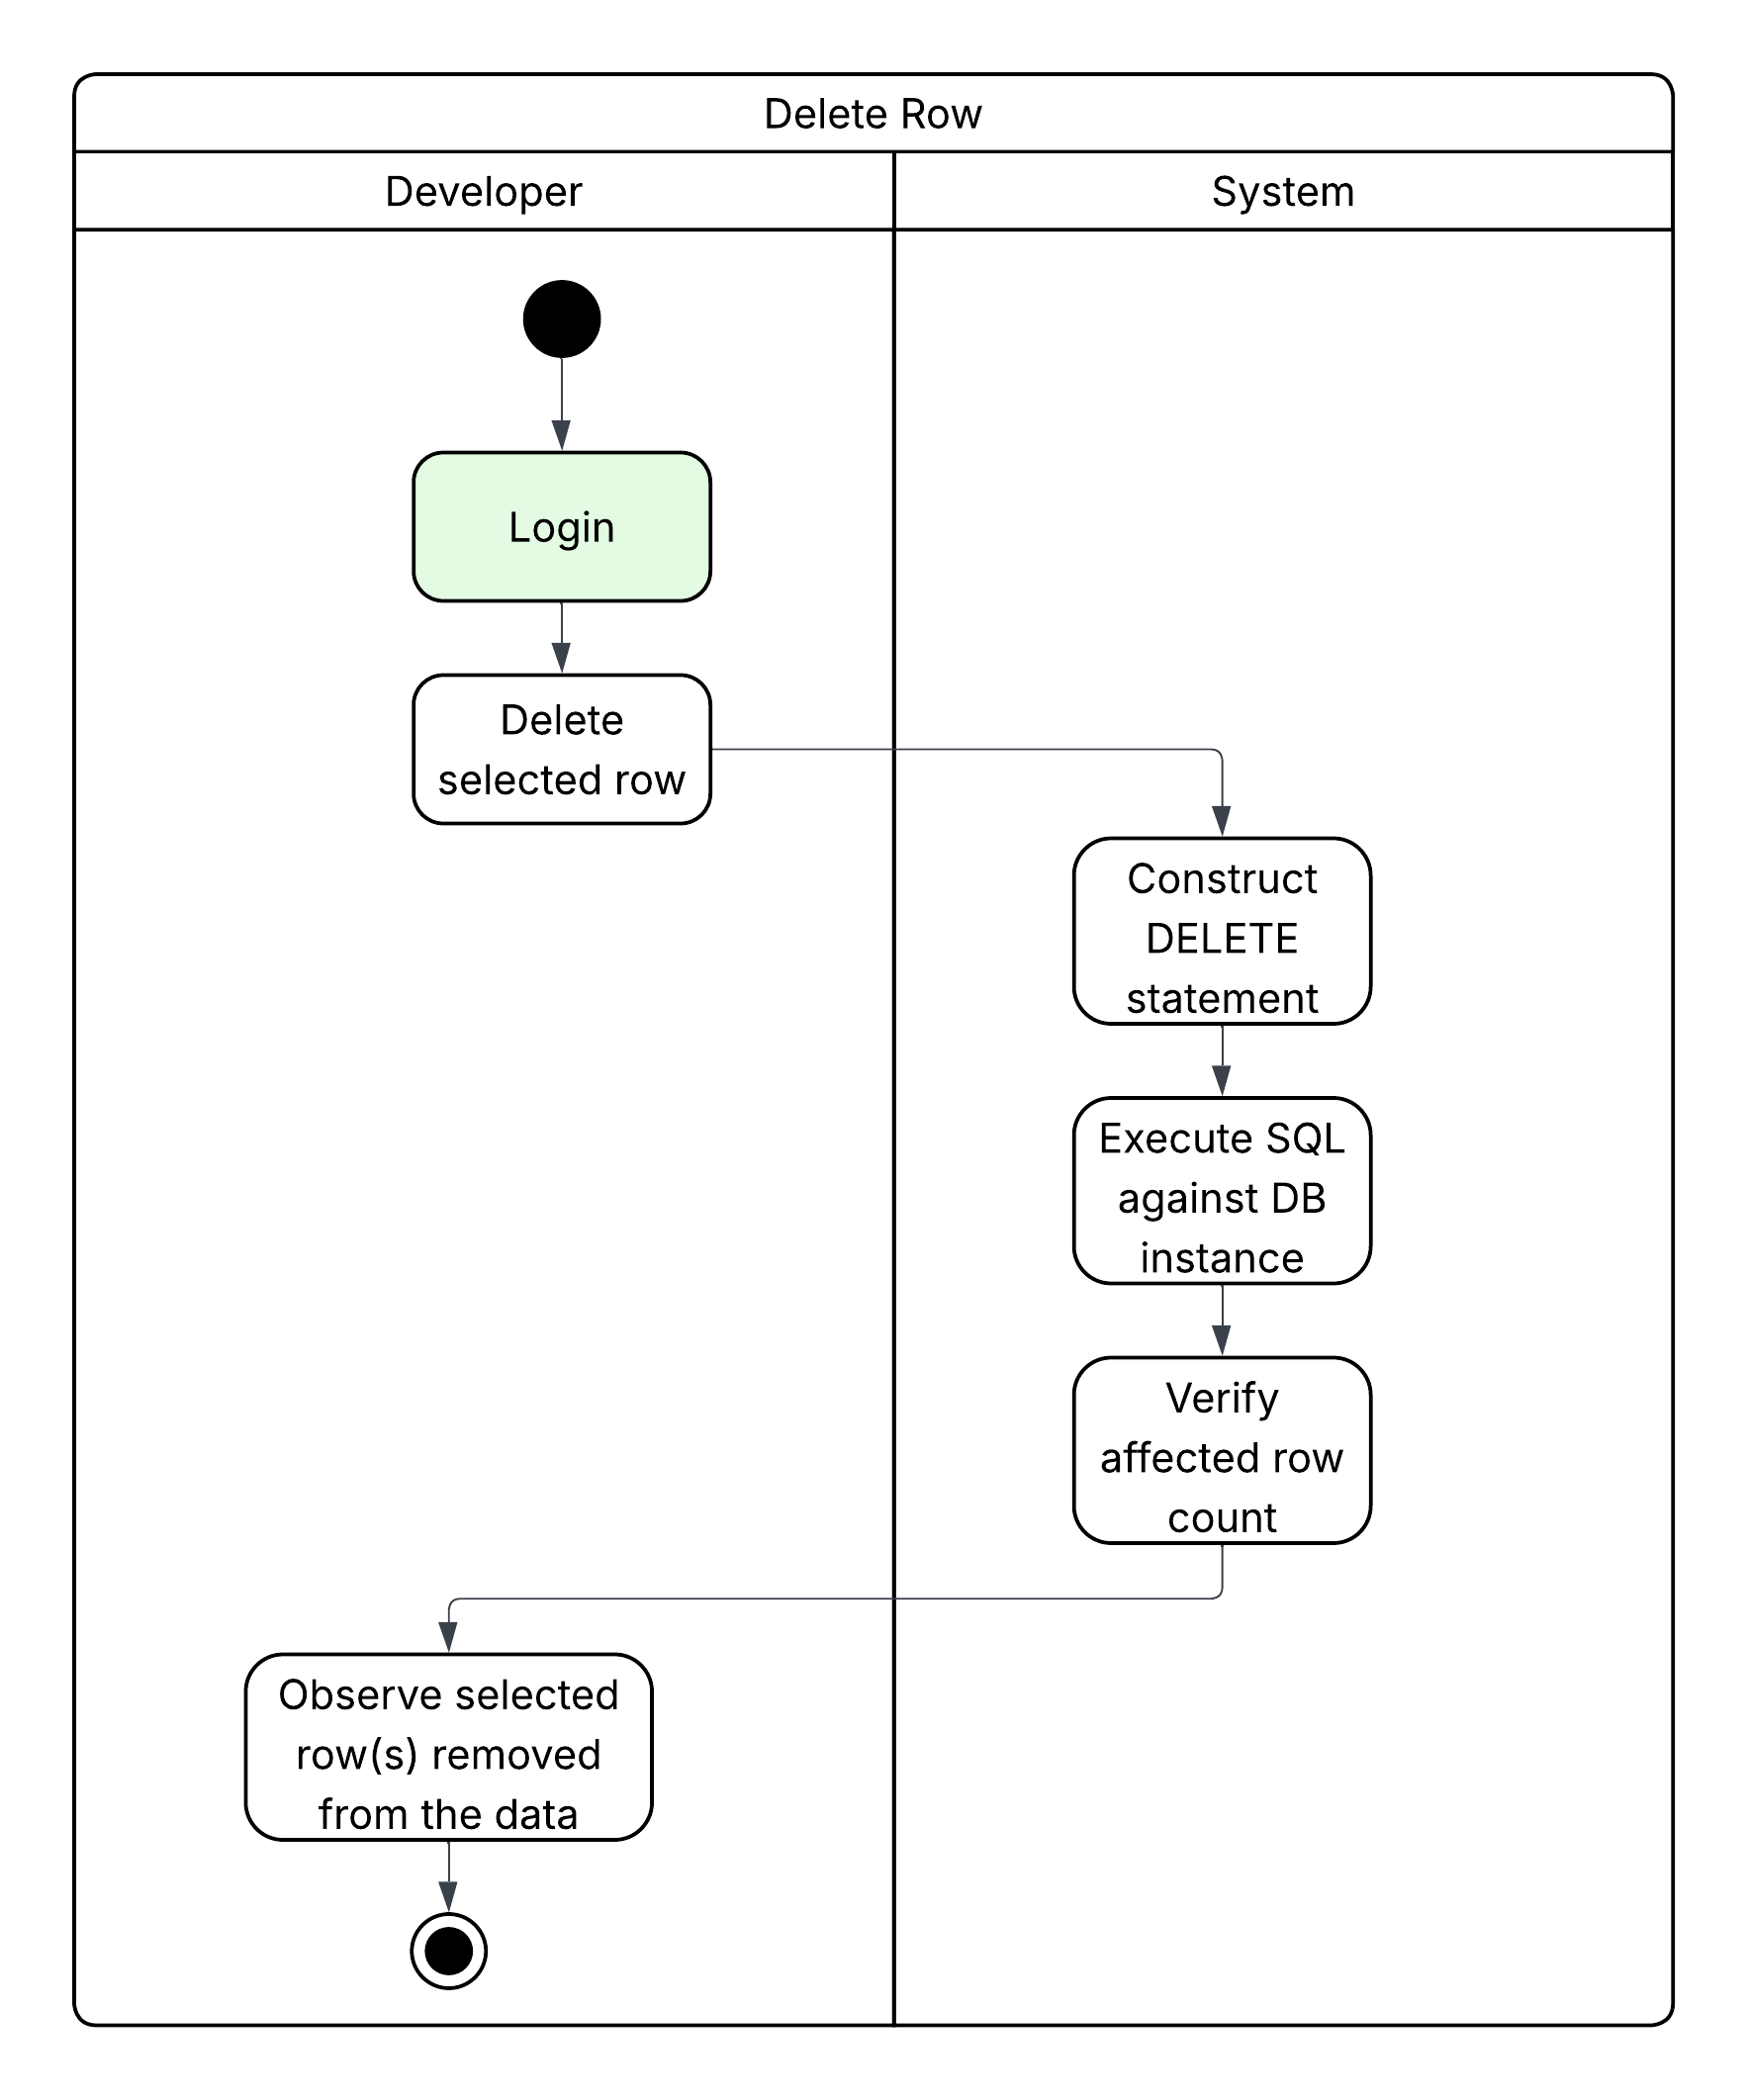
\includegraphics{images/activity/2.Delete_Row.png}
        \caption{Delete SQL rows activity diagram}
        \label{fig:delete_rows_activity}
    \end{figure}

    \begin{figure}[H]
        \centering
        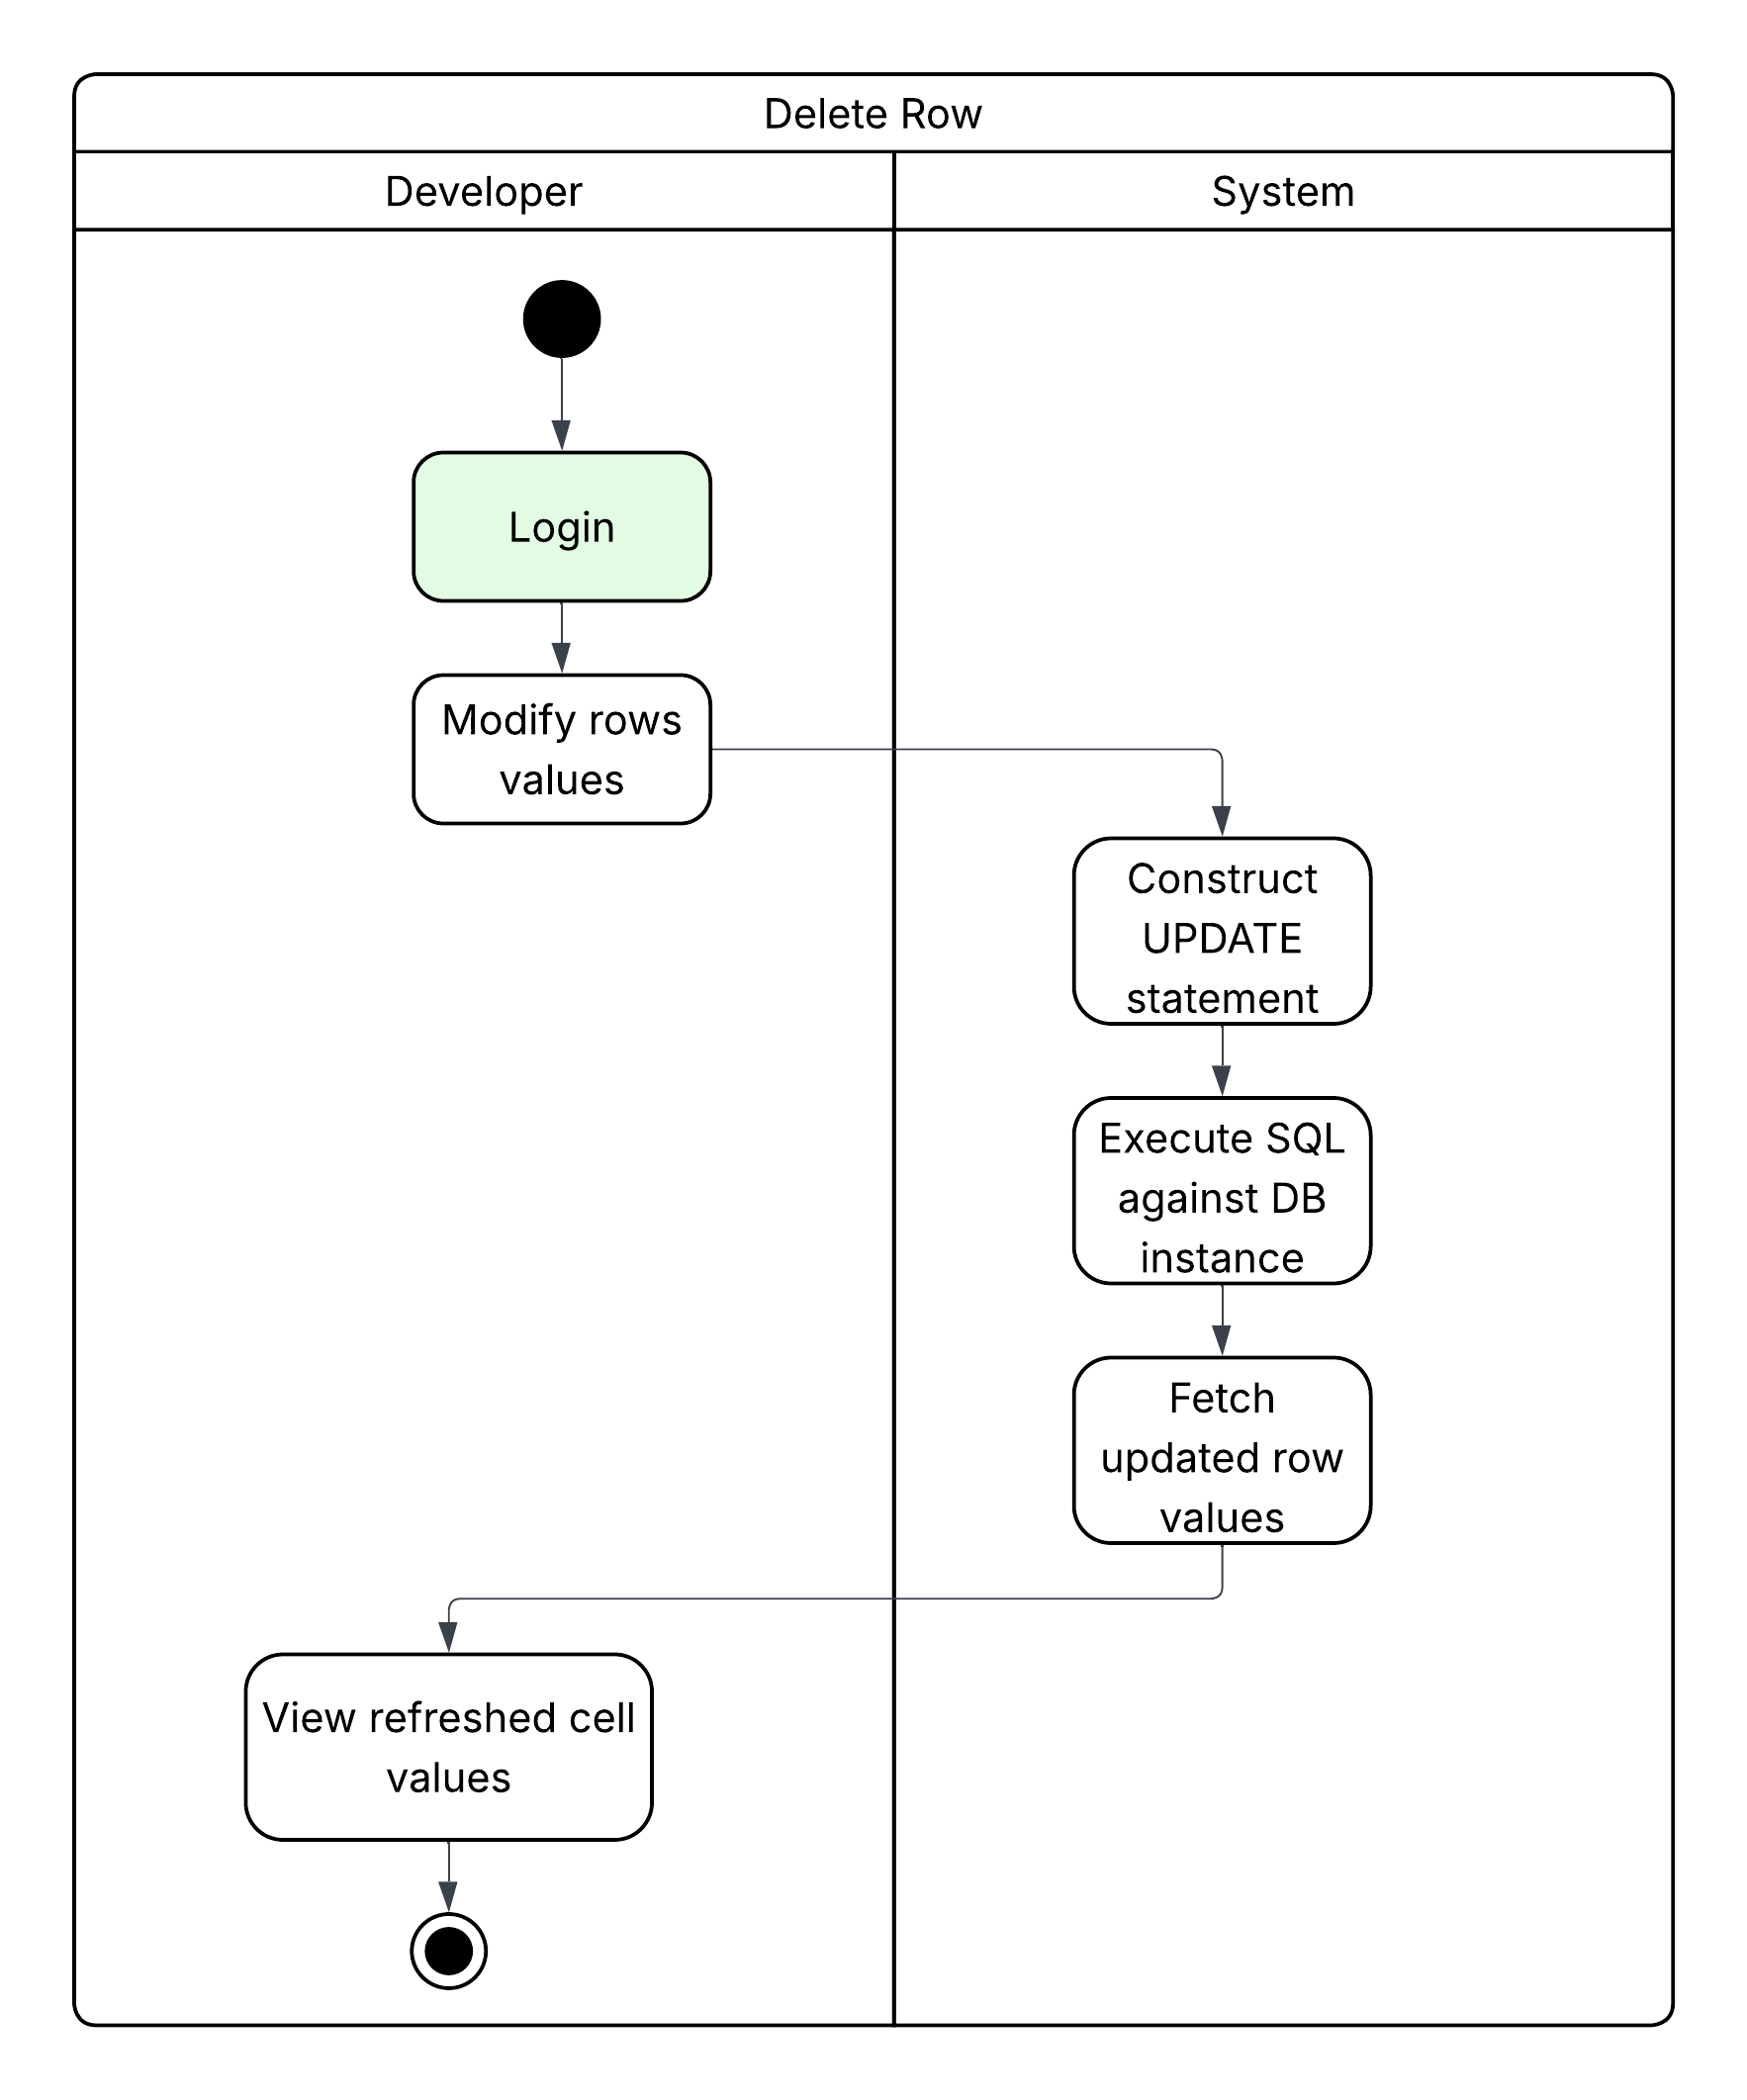
\includegraphics{images/activity/3.Edit_Row.png}
        \caption{Edit SQL rows activity diagram}
        \label{fig:edit_rows_activity}
    \end{figure}

    \begin{figure}[H]
        \centering
        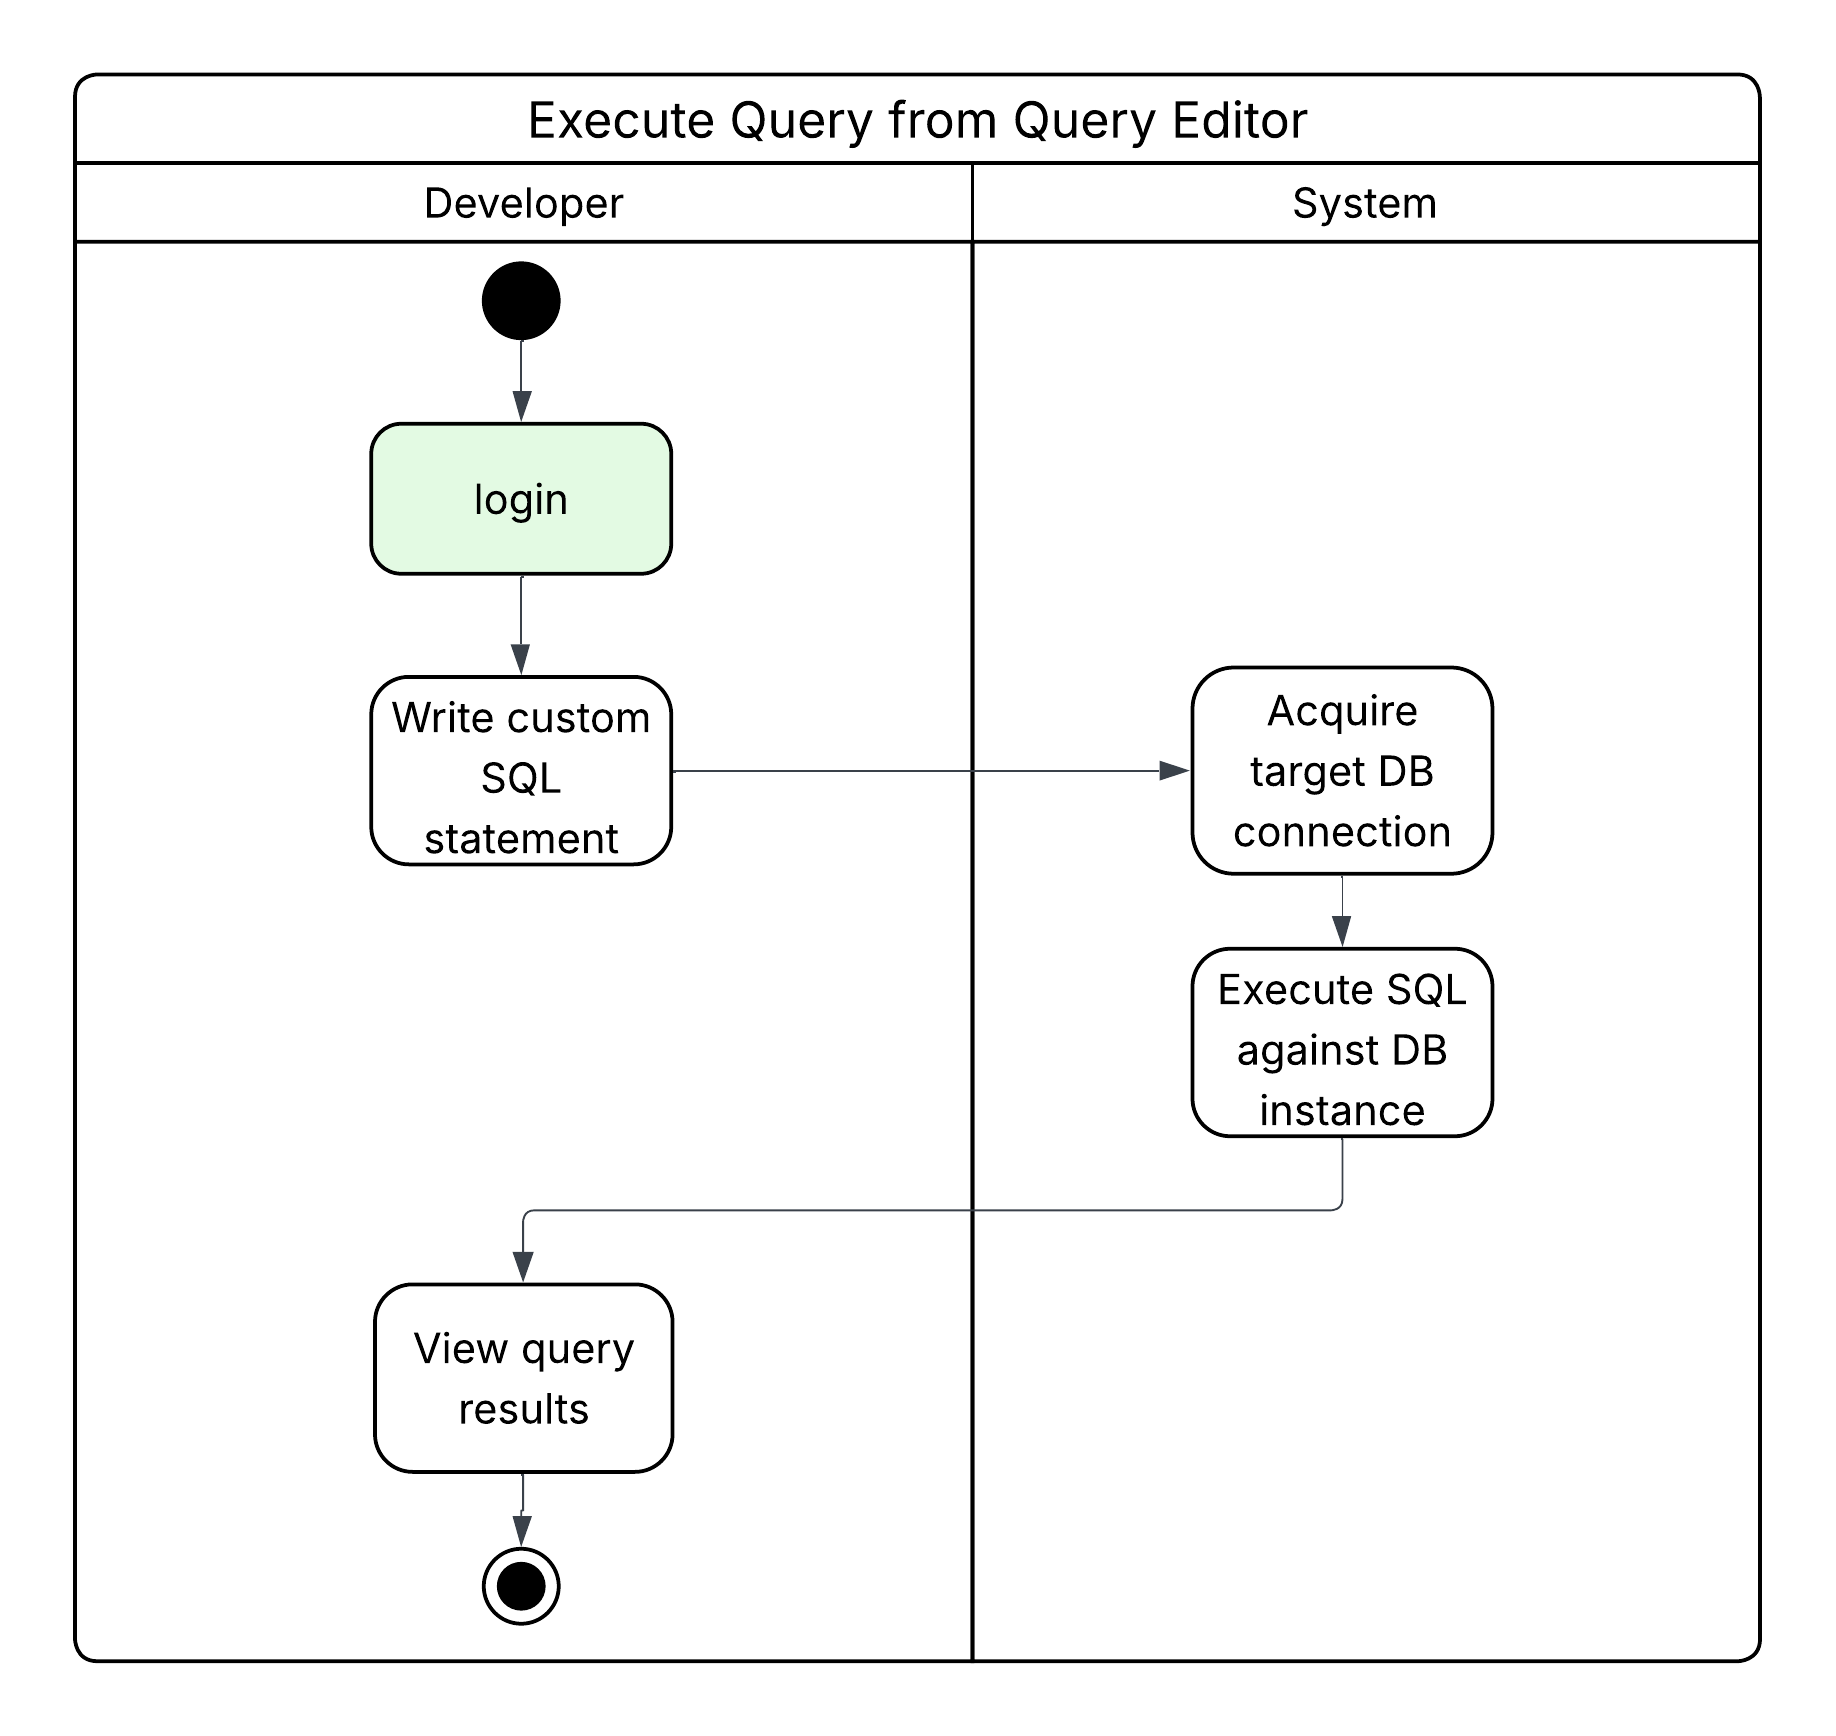
\includegraphics{images/activity/7.Execute_Query_from_Query_Editor.png}
        \caption{Execute SQL query activity diagram}
        \label{fig:Execute_Query_from_Query_Editor}
    \end{figure}

    % \begin{figure}[H]
    %     \centering
    %     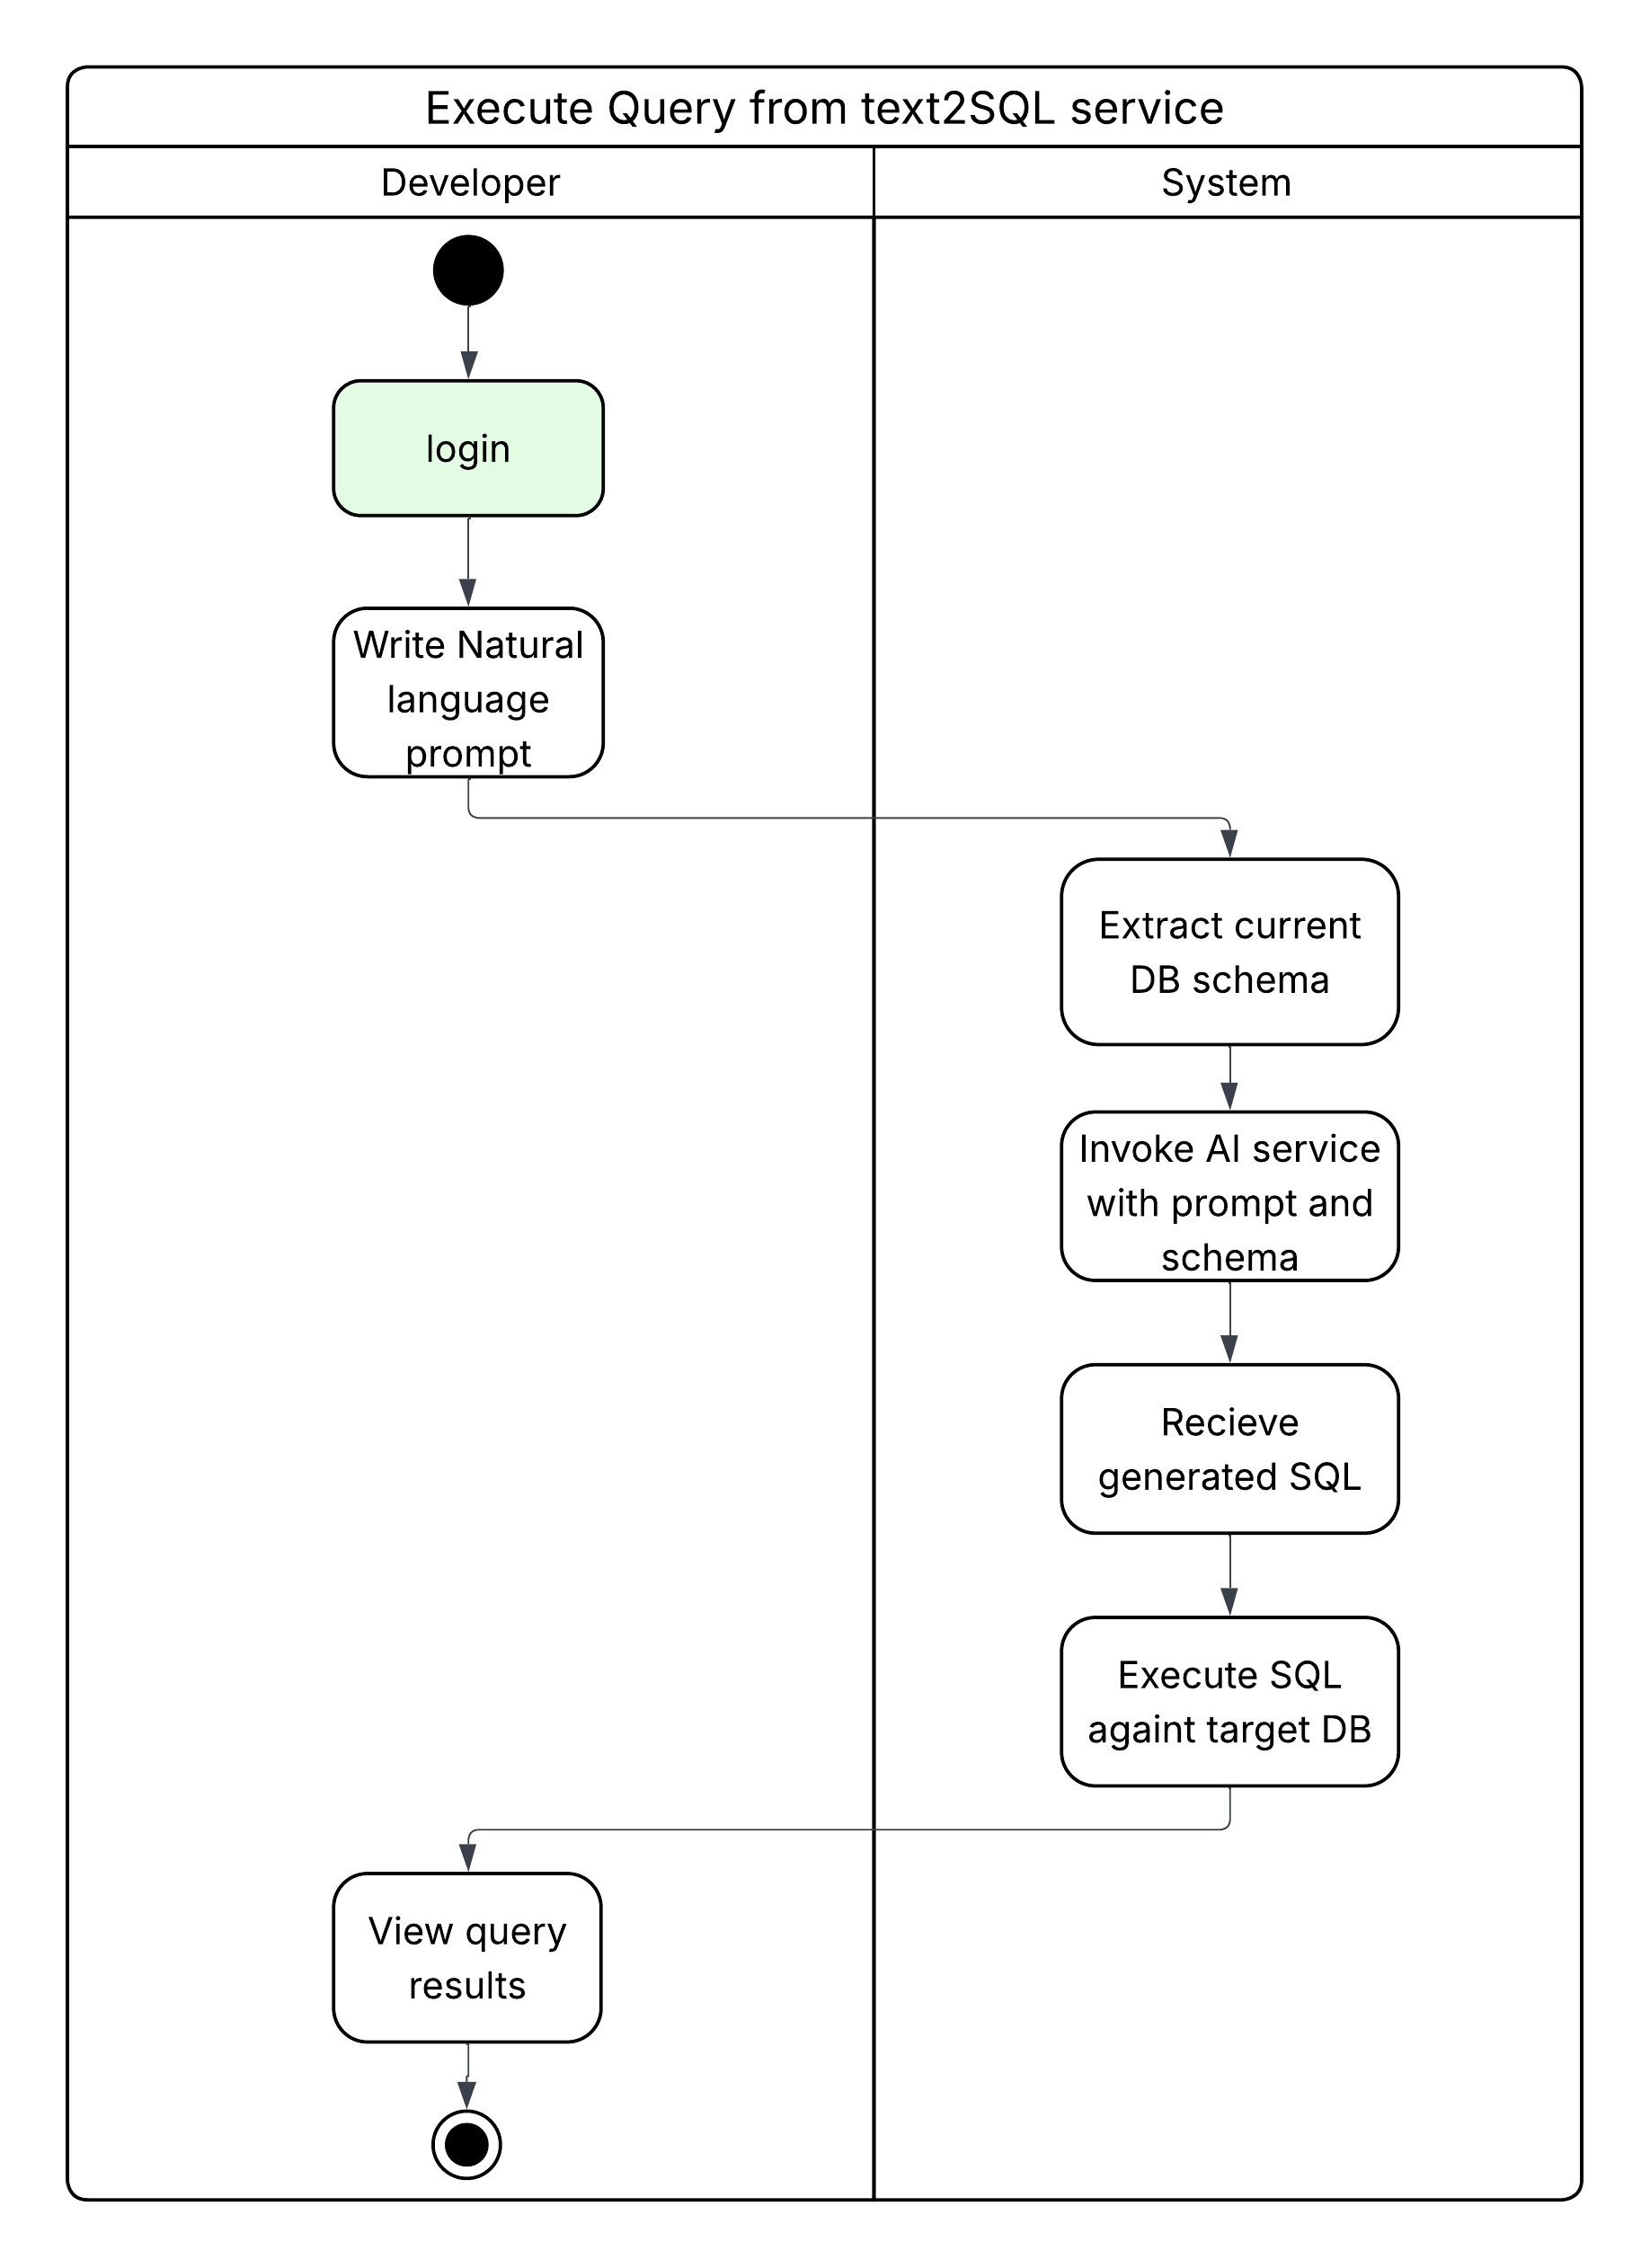
\includegraphics{images/activity/8.Execute_Query_via_Text2SQL_AI_Service.png}
    %     \caption{Execute SQL query via AI activity diagram}
    %     \label{fig:Execute_Query_via_Text2SQL_AI_Service}
    % \end{figure}

    \begin{figure}[H]
        \centering
        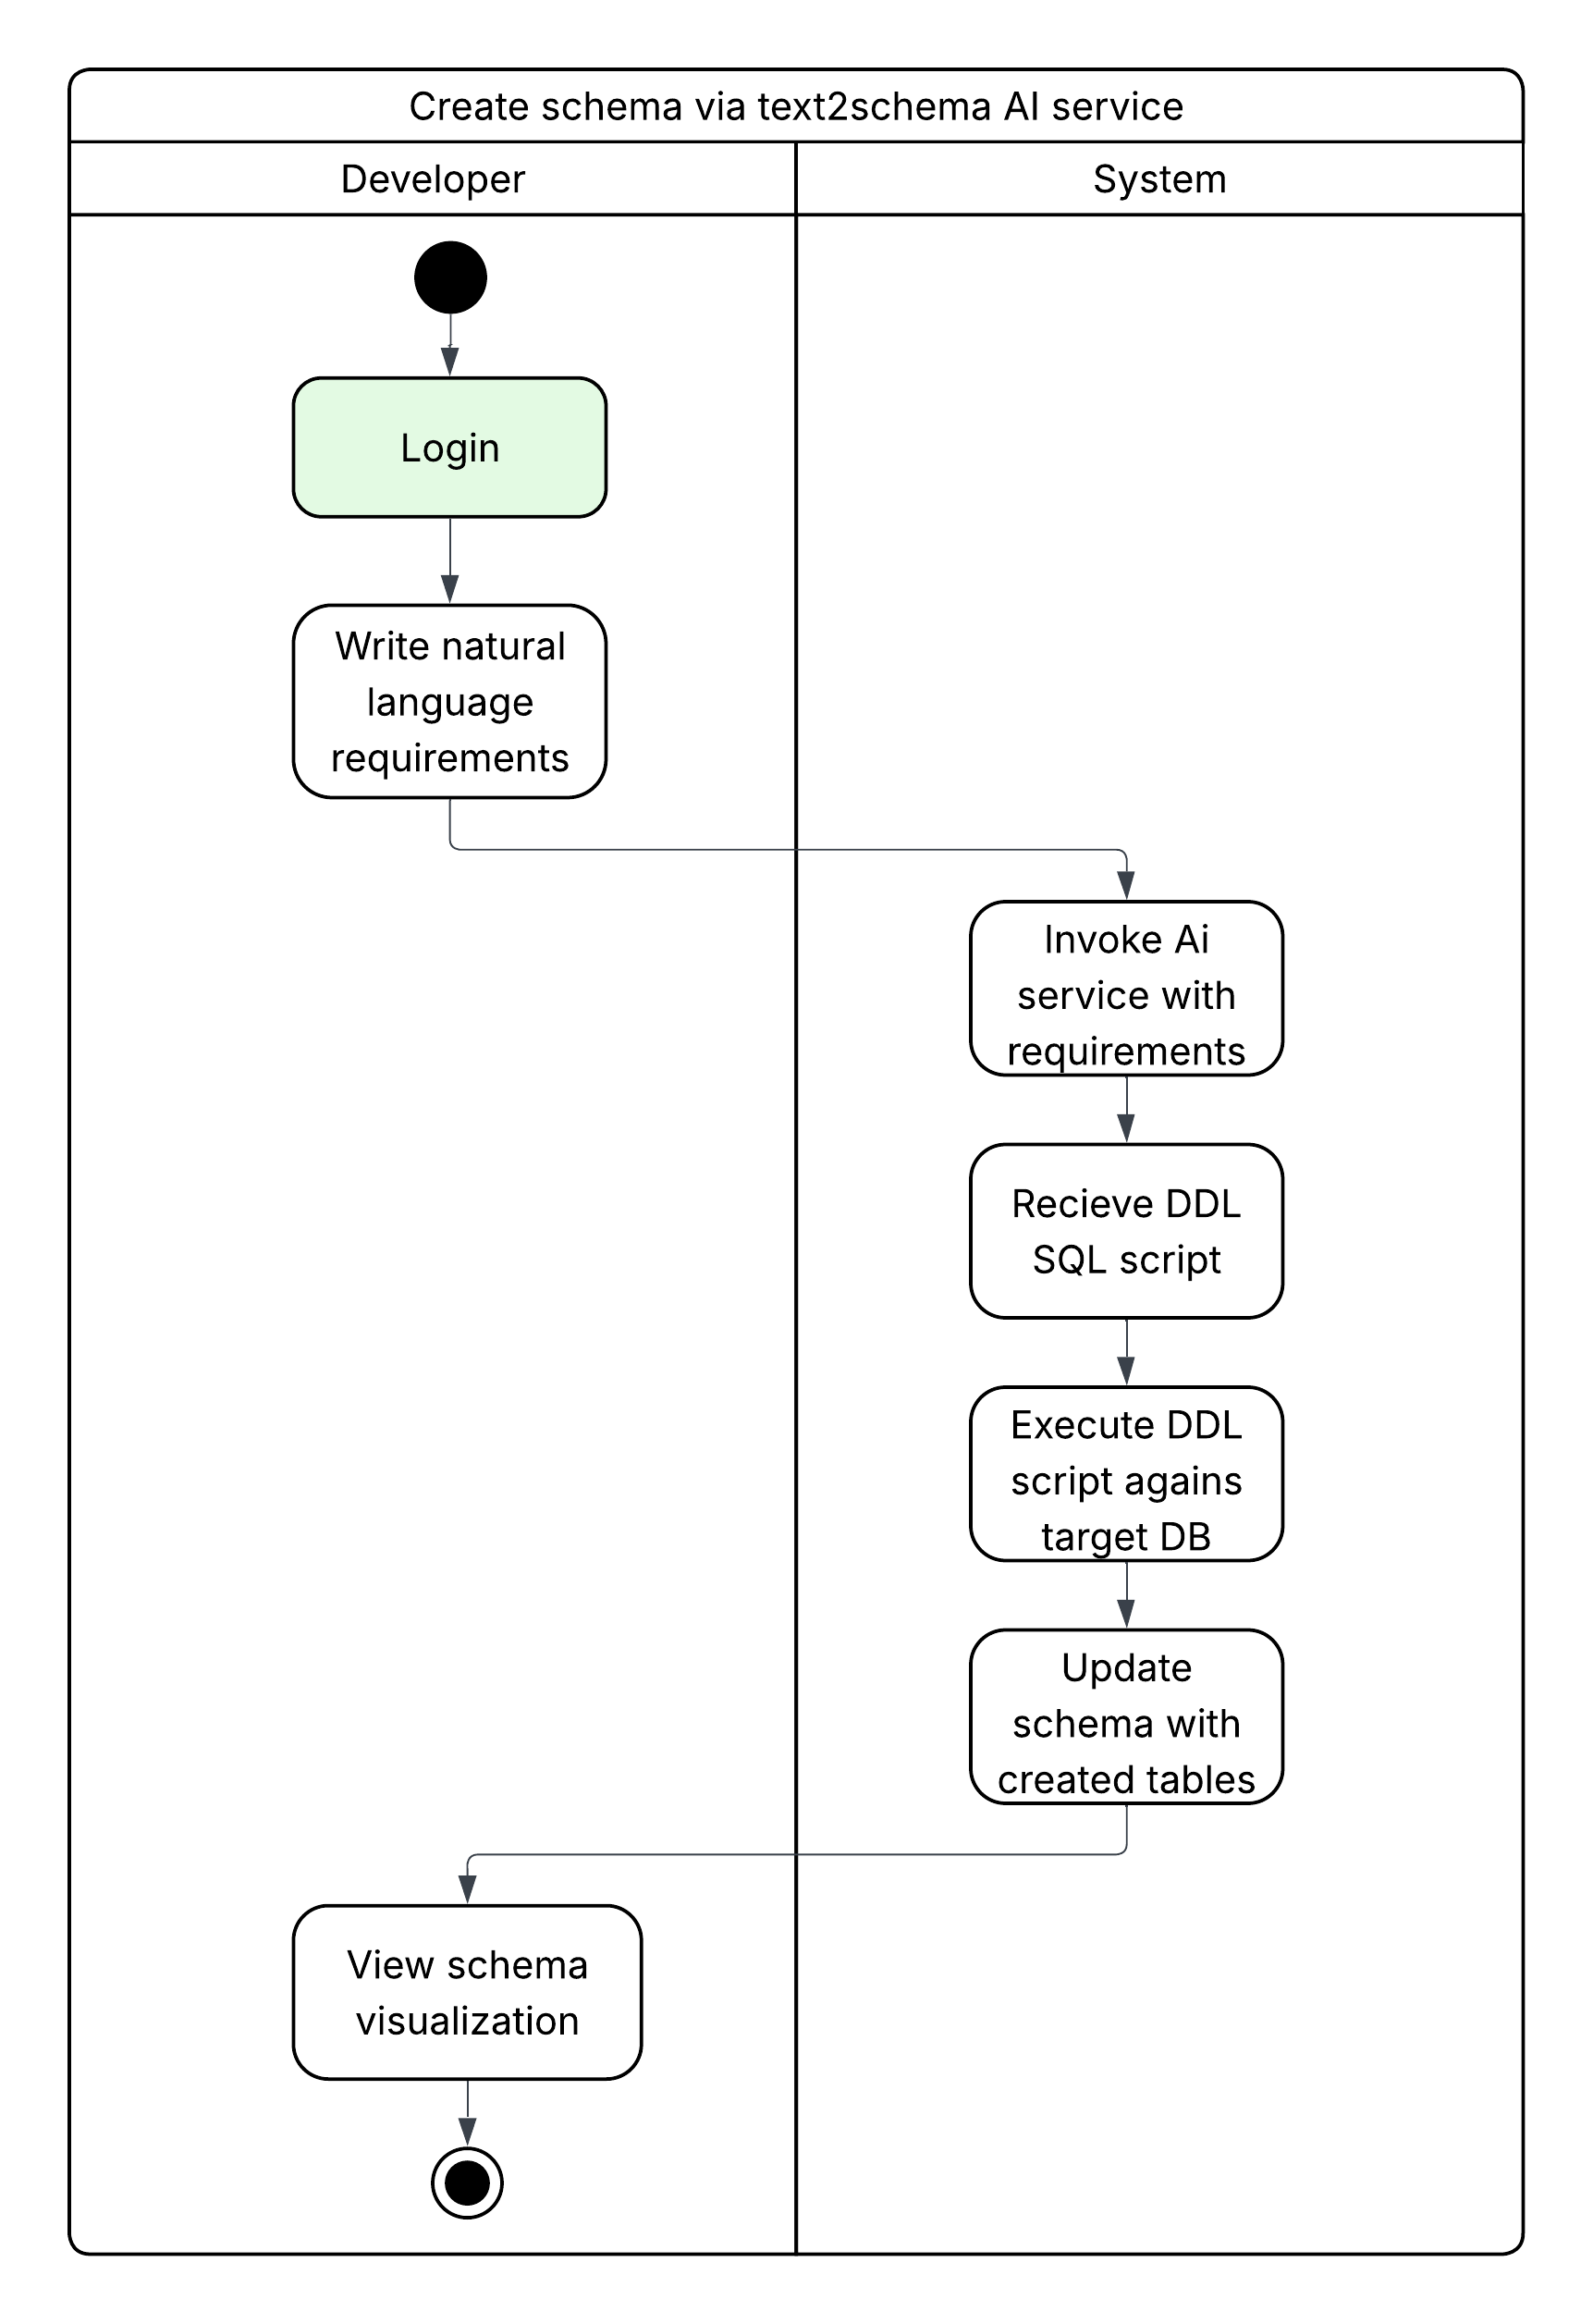
\includegraphics{images/activity/9.Create_Schema_via_Text2Schema_AI_Service.png}
        \caption{Create SQL schema via AI activity diagram}
        \label{fig:Create_Schema_via_Text2Schema_AI_Service}
    \end{figure}

    \begin{figure}[H]
        \centering
        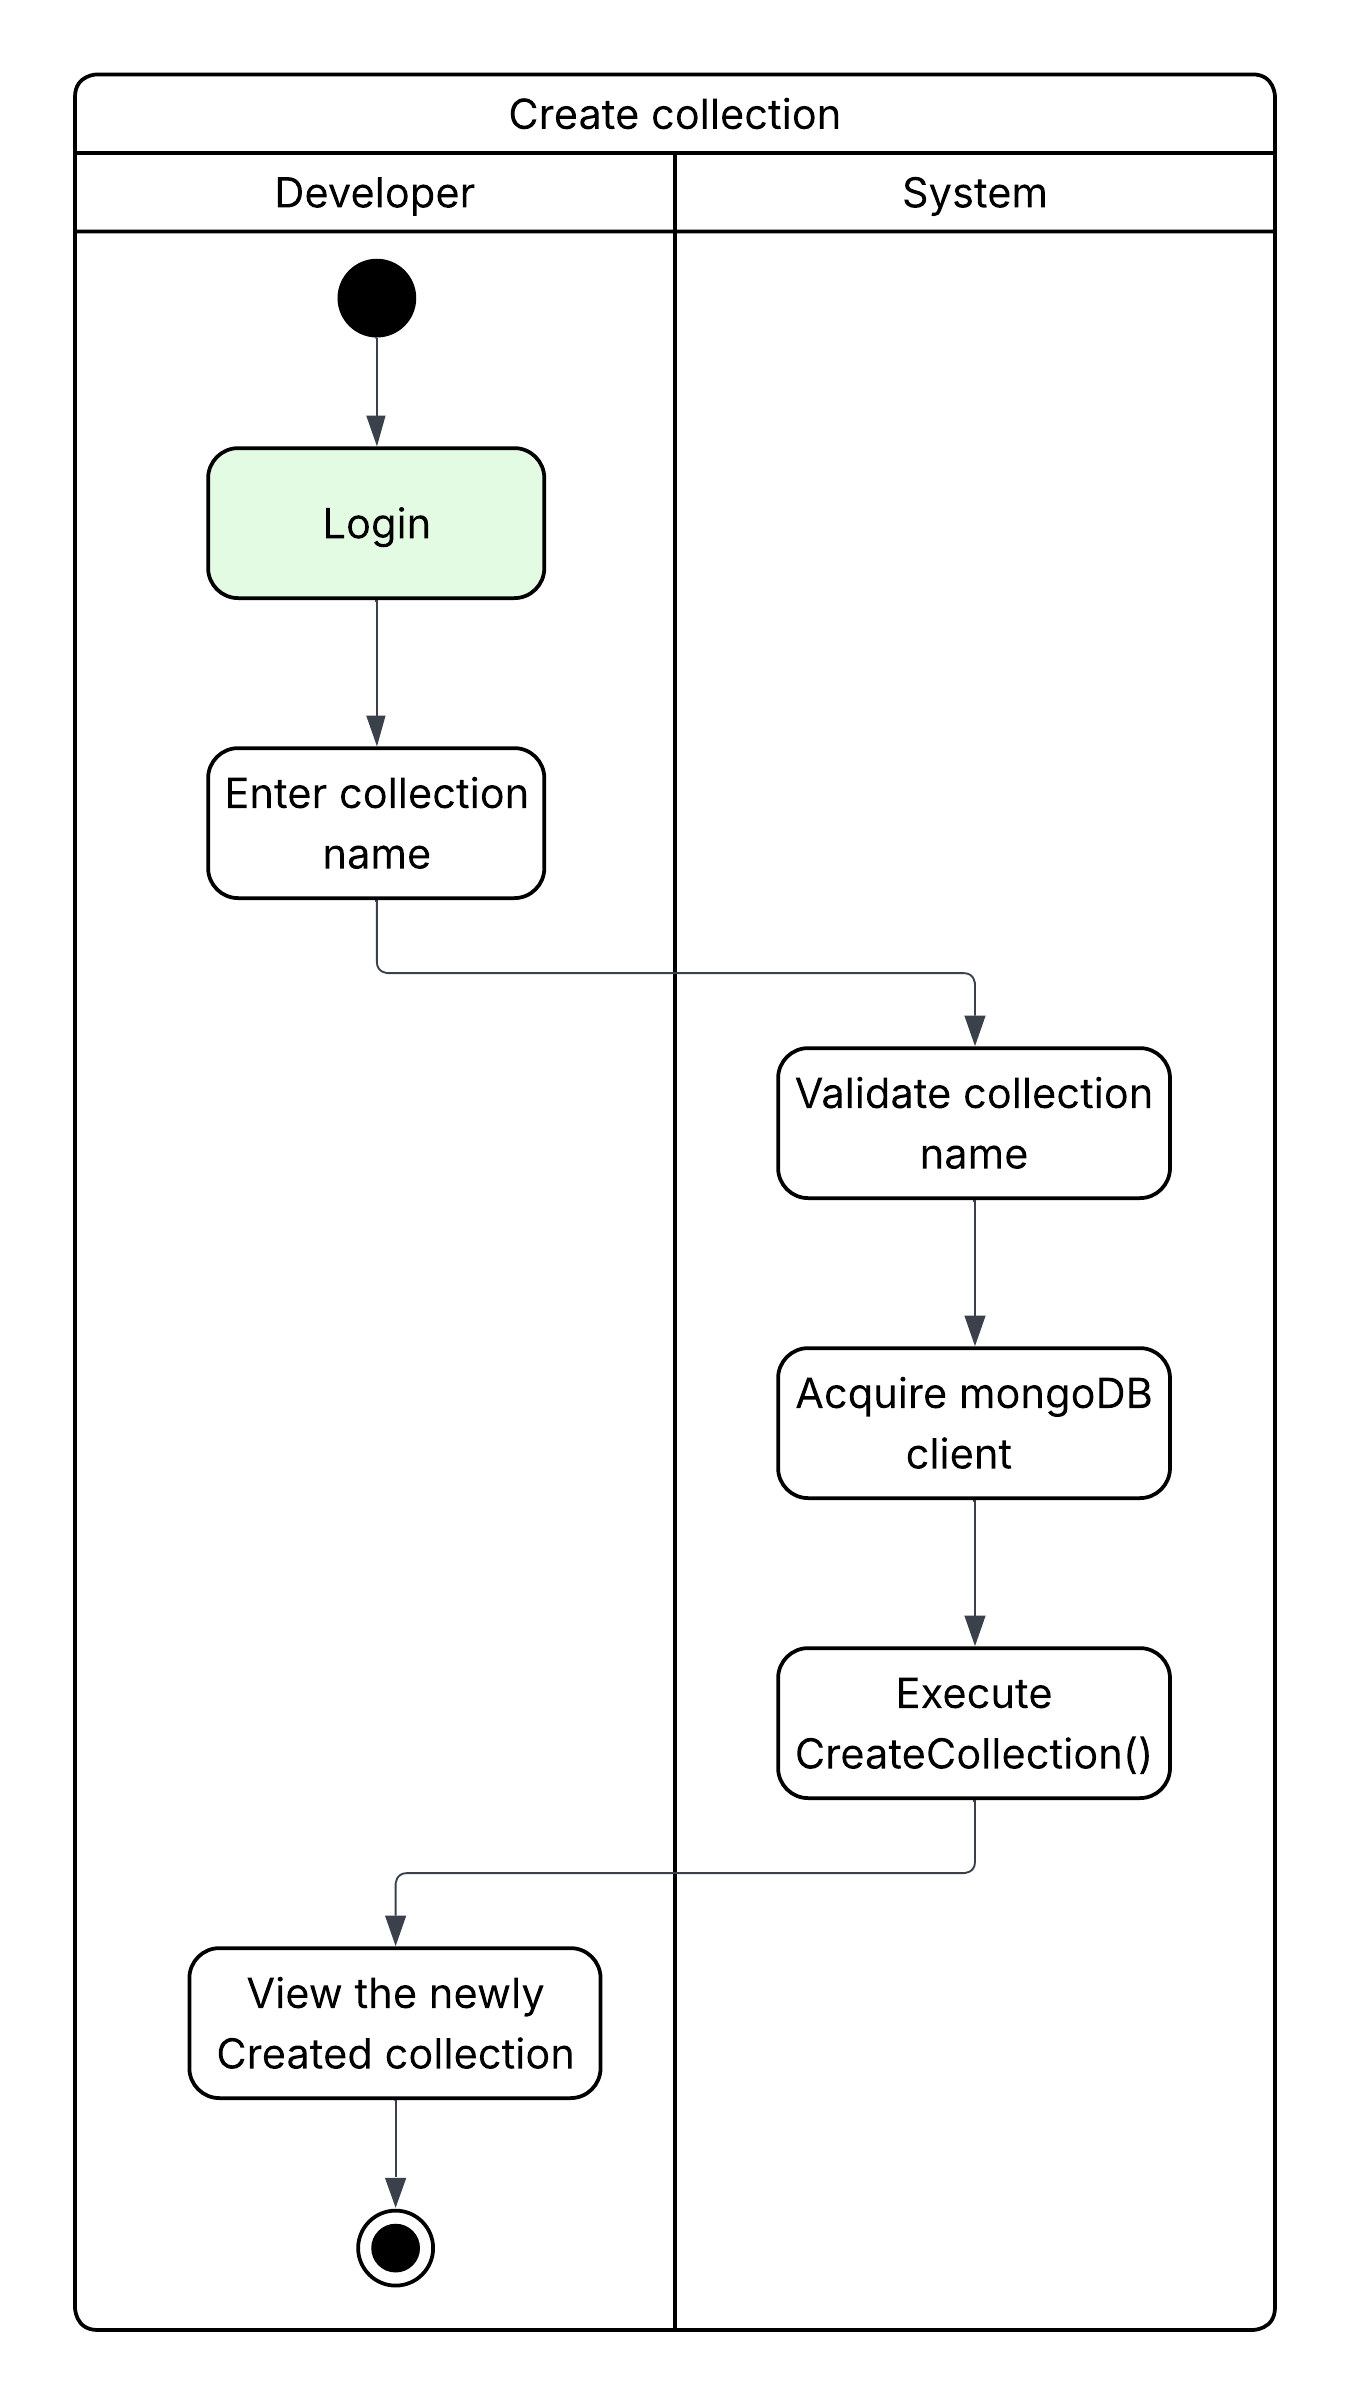
\includegraphics{images/activity/10.Create_collection.png}
        \caption{Create NoSQL collection activity diagram}
        \label{fig:Create_collection}
    \end{figure}

    \begin{figure}[H]
        \centering
        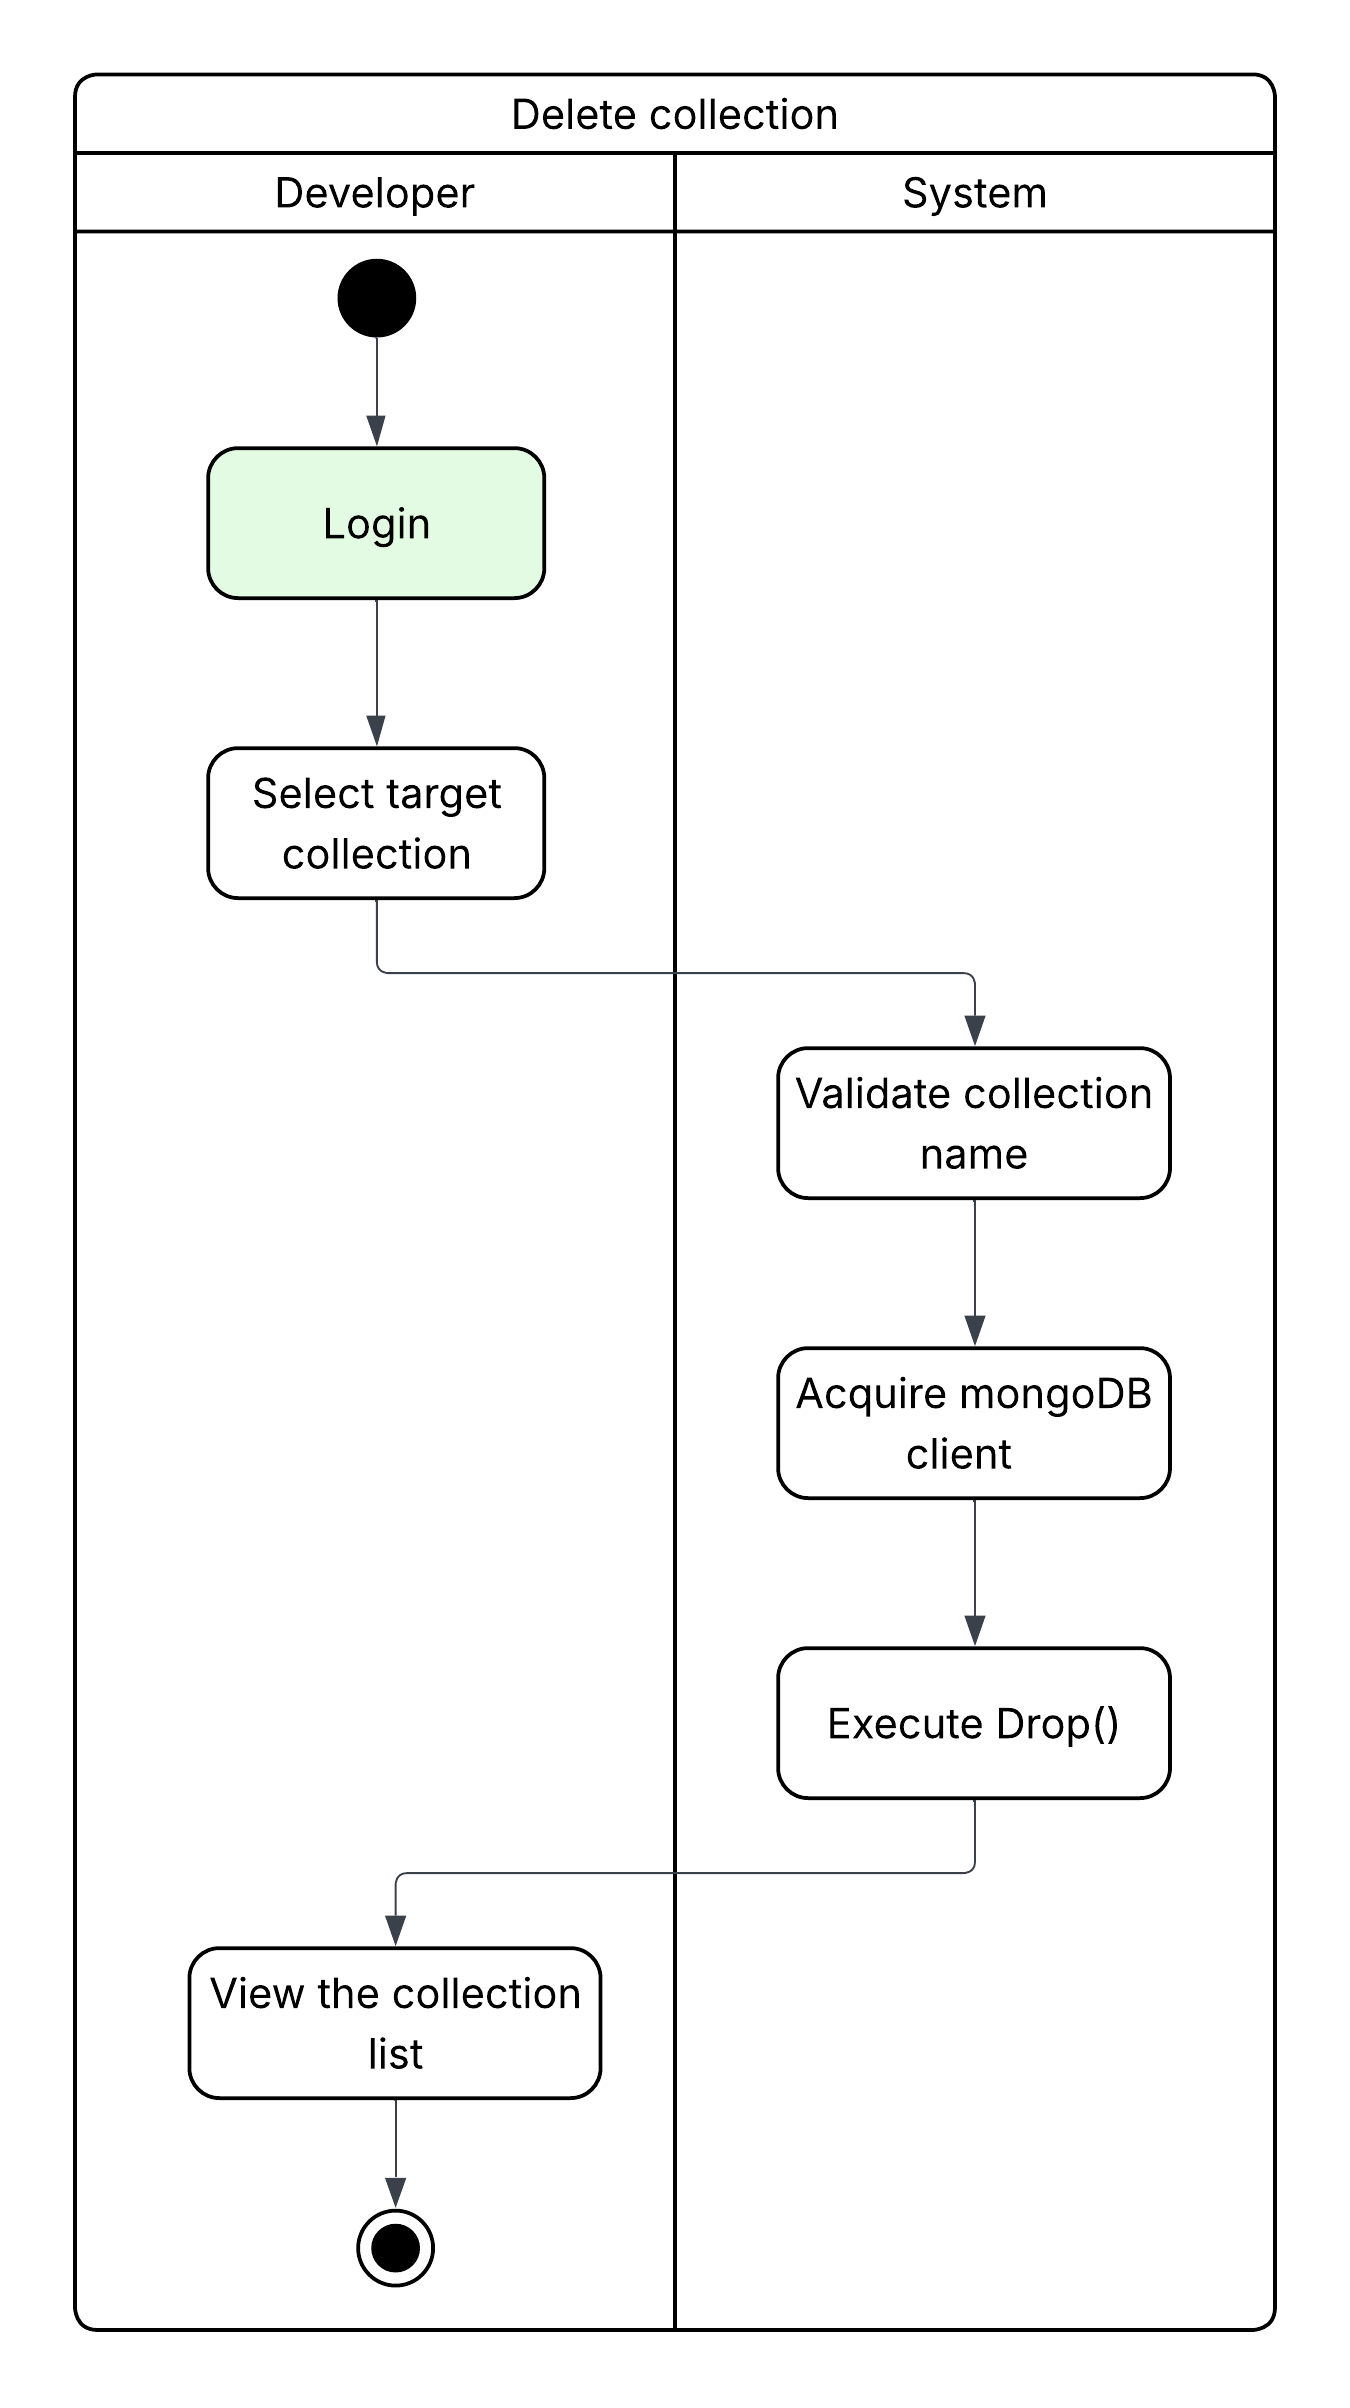
\includegraphics{images/activity/11.Delete_Collection.png}
        \caption{Delete NoSQL collection activity diagram}
        \label{fig:Delete_Collection}
    \end{figure}

    \begin{figure}[H]
        \centering
        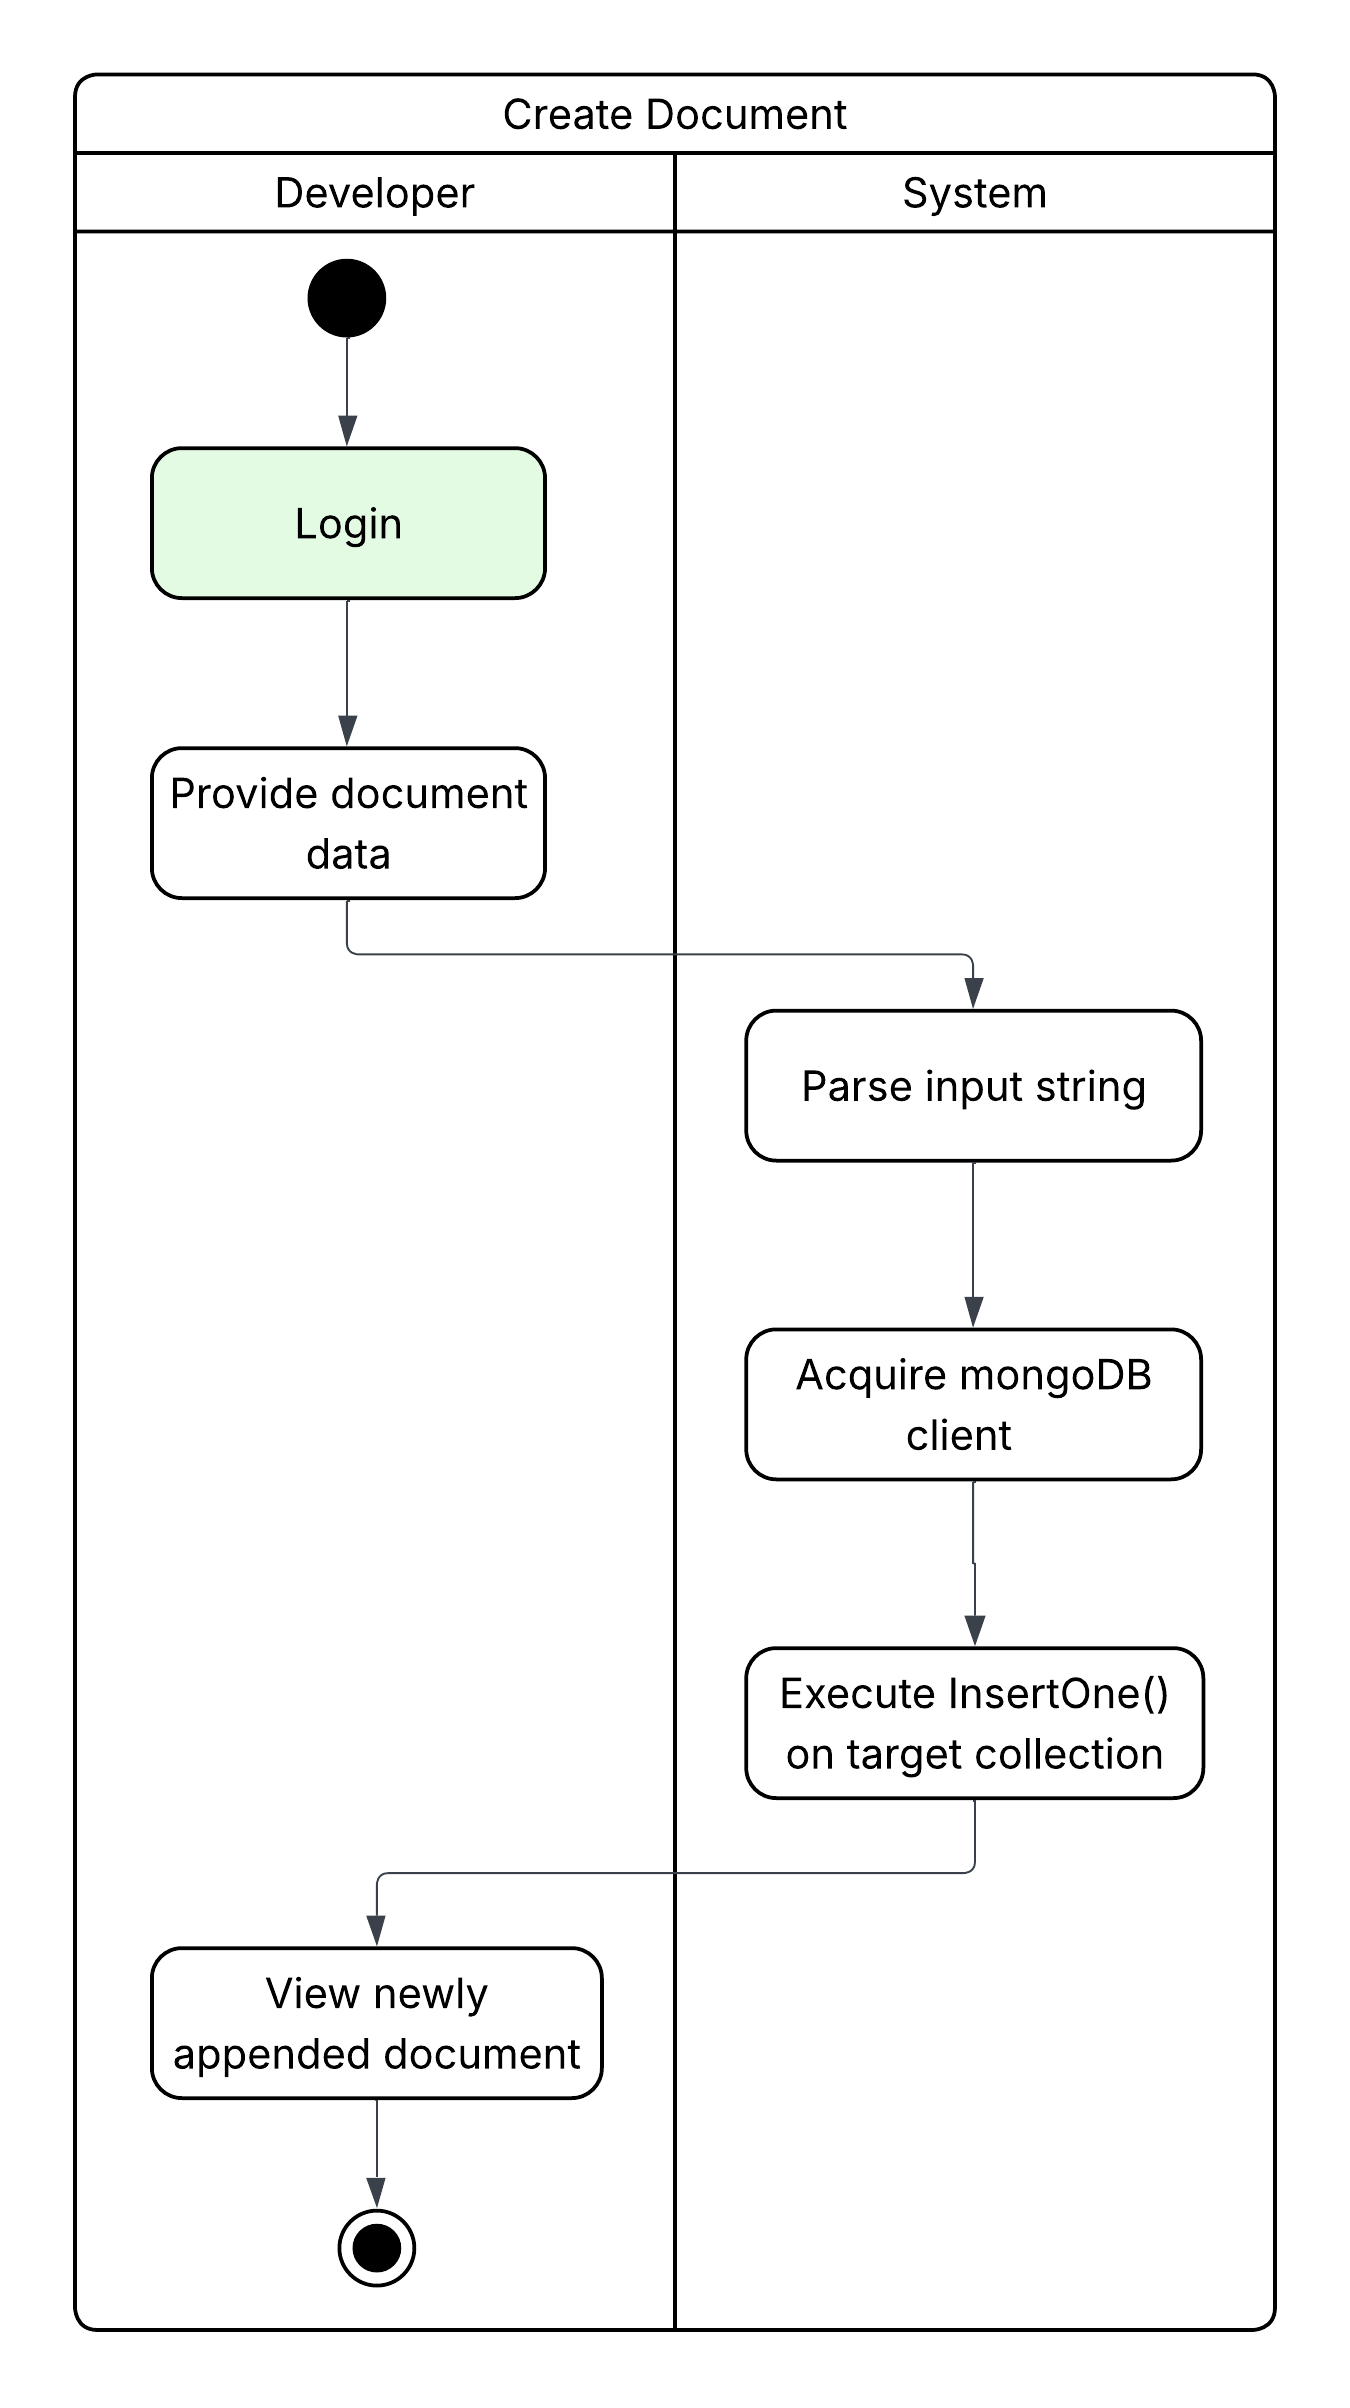
\includegraphics{images/activity/13.Create_Document.png}
        \caption{Create NoSQL document activity diagram}
        \label{fig:Create_Document}
    \end{figure}

    \begin{figure}[H]
        \centering
        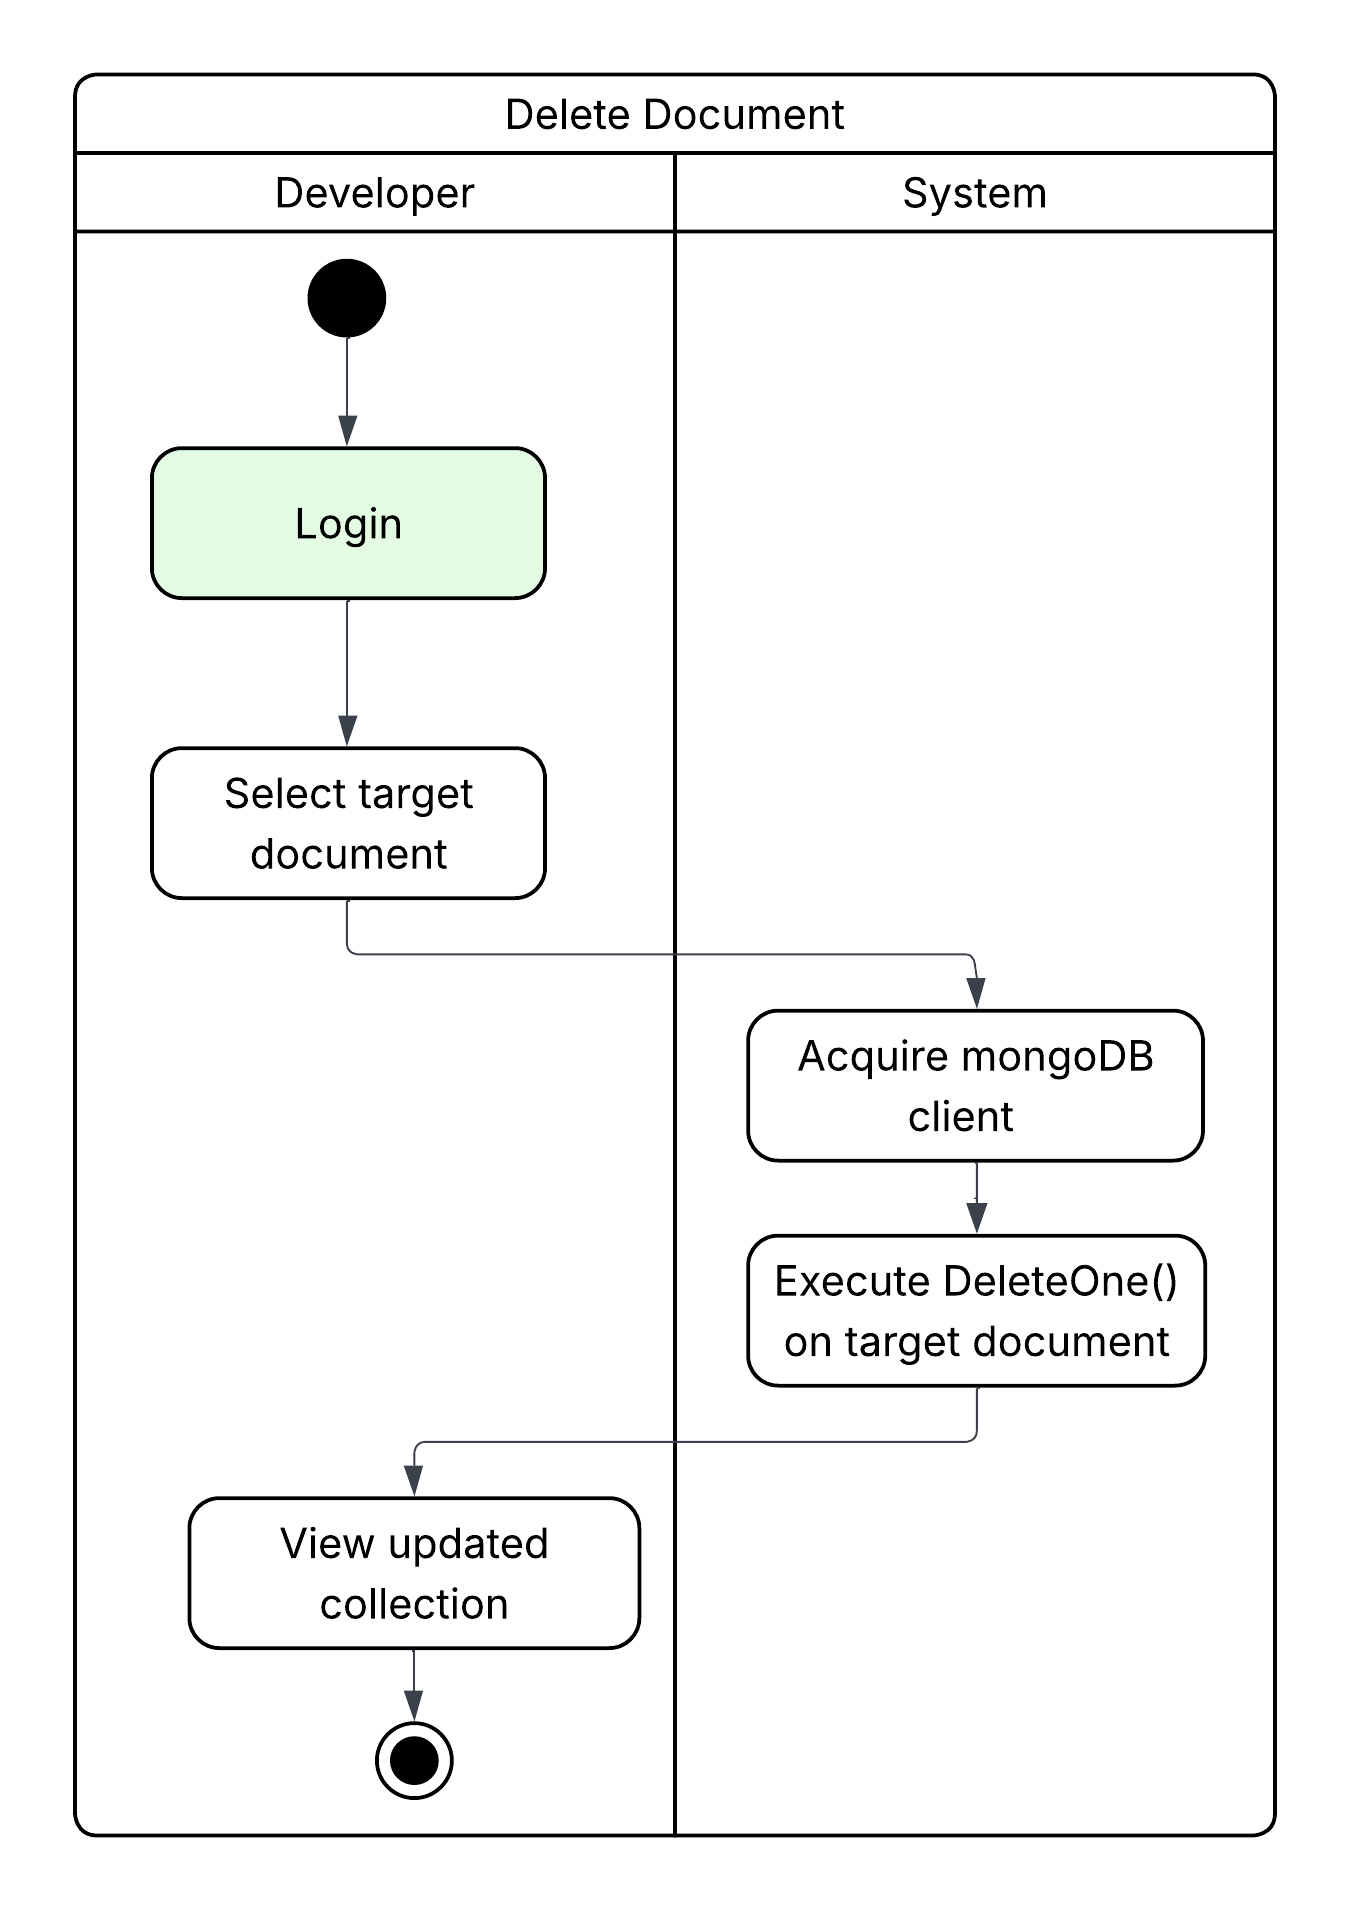
\includegraphics{images/activity/14.Delete_Document.png}
        \caption{Delete NoSQL document activity diagram}
        \label{fig:Delete_Document}
    \end{figure}

    \begin{figure}[H]
        \centering
        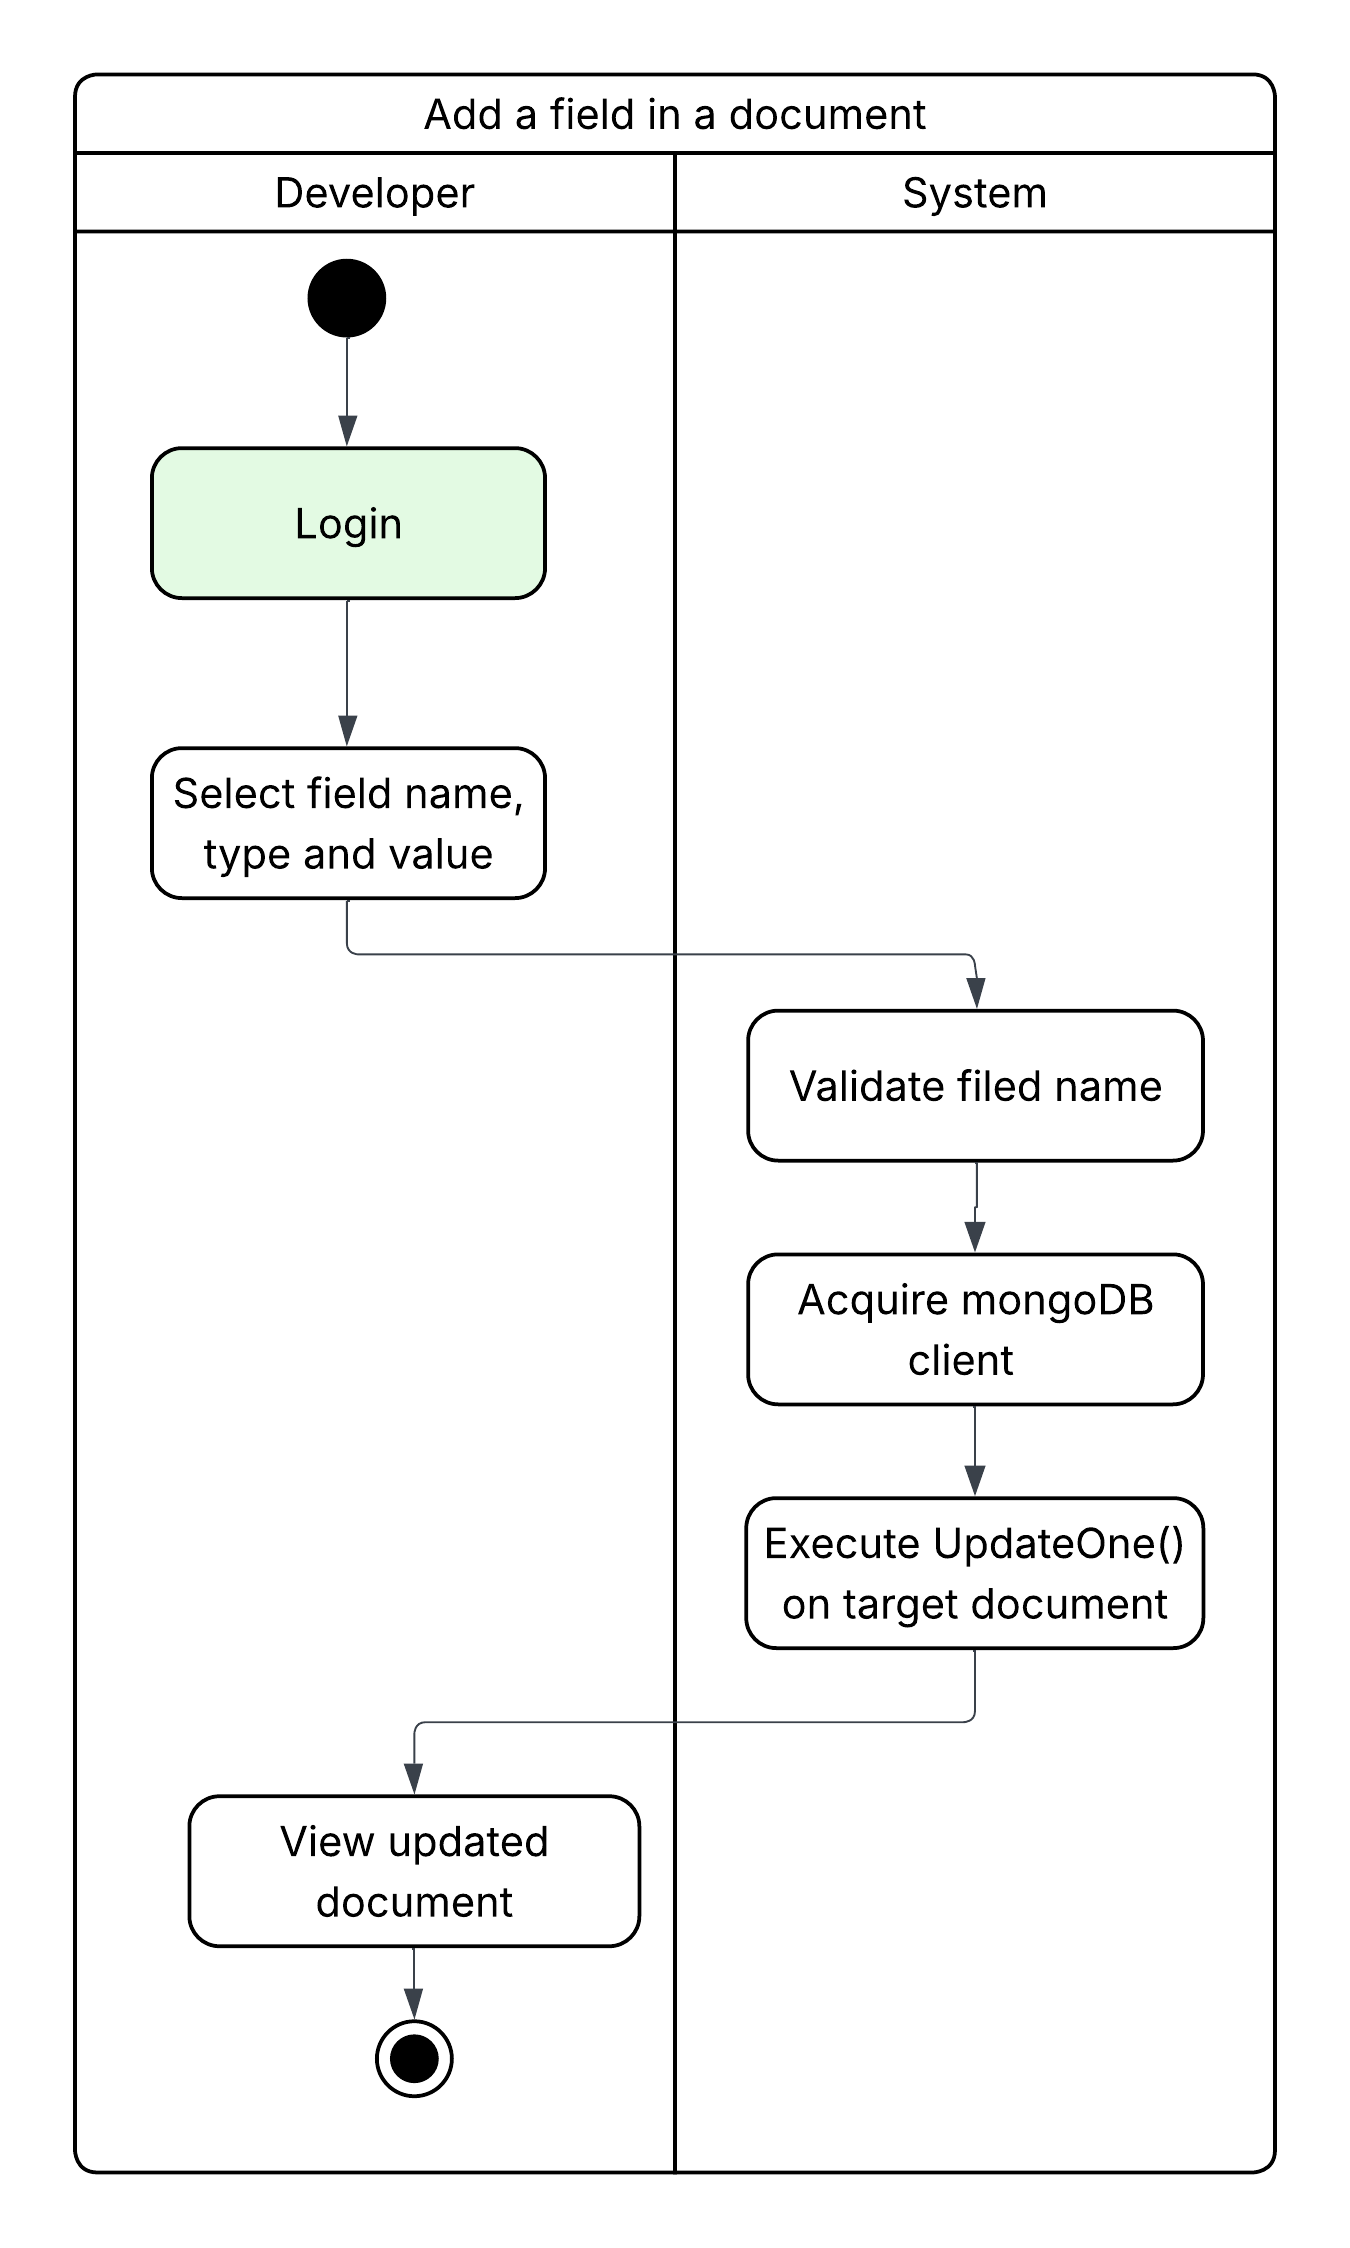
\includegraphics{images/activity/15.Add_a_Field_in_a_Document.png}
        \caption{Add a NoSQL field in a document activity diagram}
        \label{fig:Add_a_Field_in_a_Document}
    \end{figure}

    \begin{figure}[H]
        \centering
        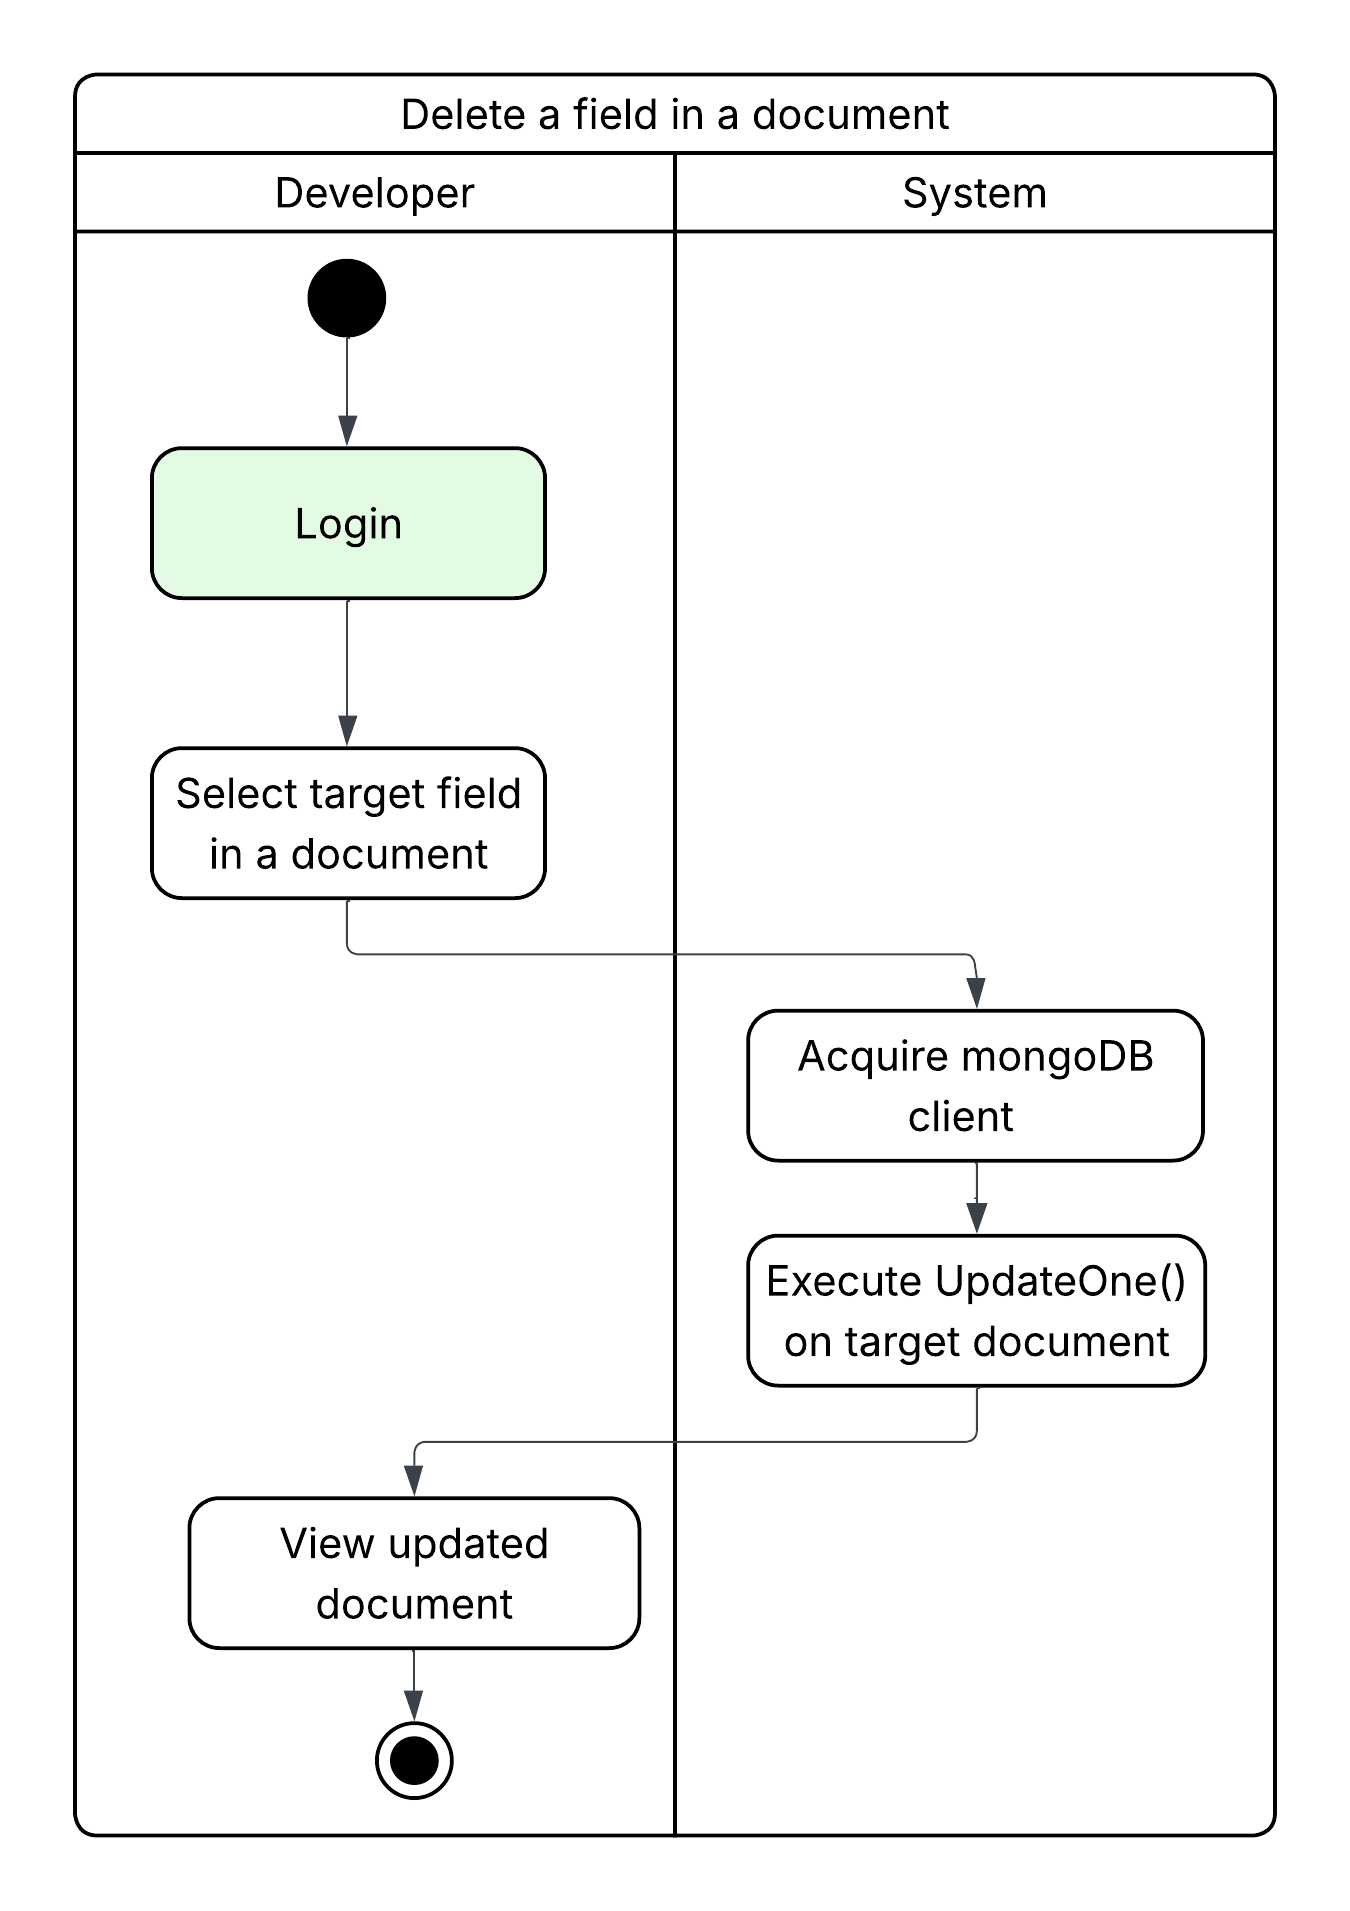
\includegraphics{images/activity/16.Delete_a_Field_in_a_Document.png}
        \caption{Delete a NoSQL field in a document activity diagram}
        \label{fig:Delete_a_Field_in_a_Document}
    \end{figure}

    \begin{figure}[H]
        \centering
        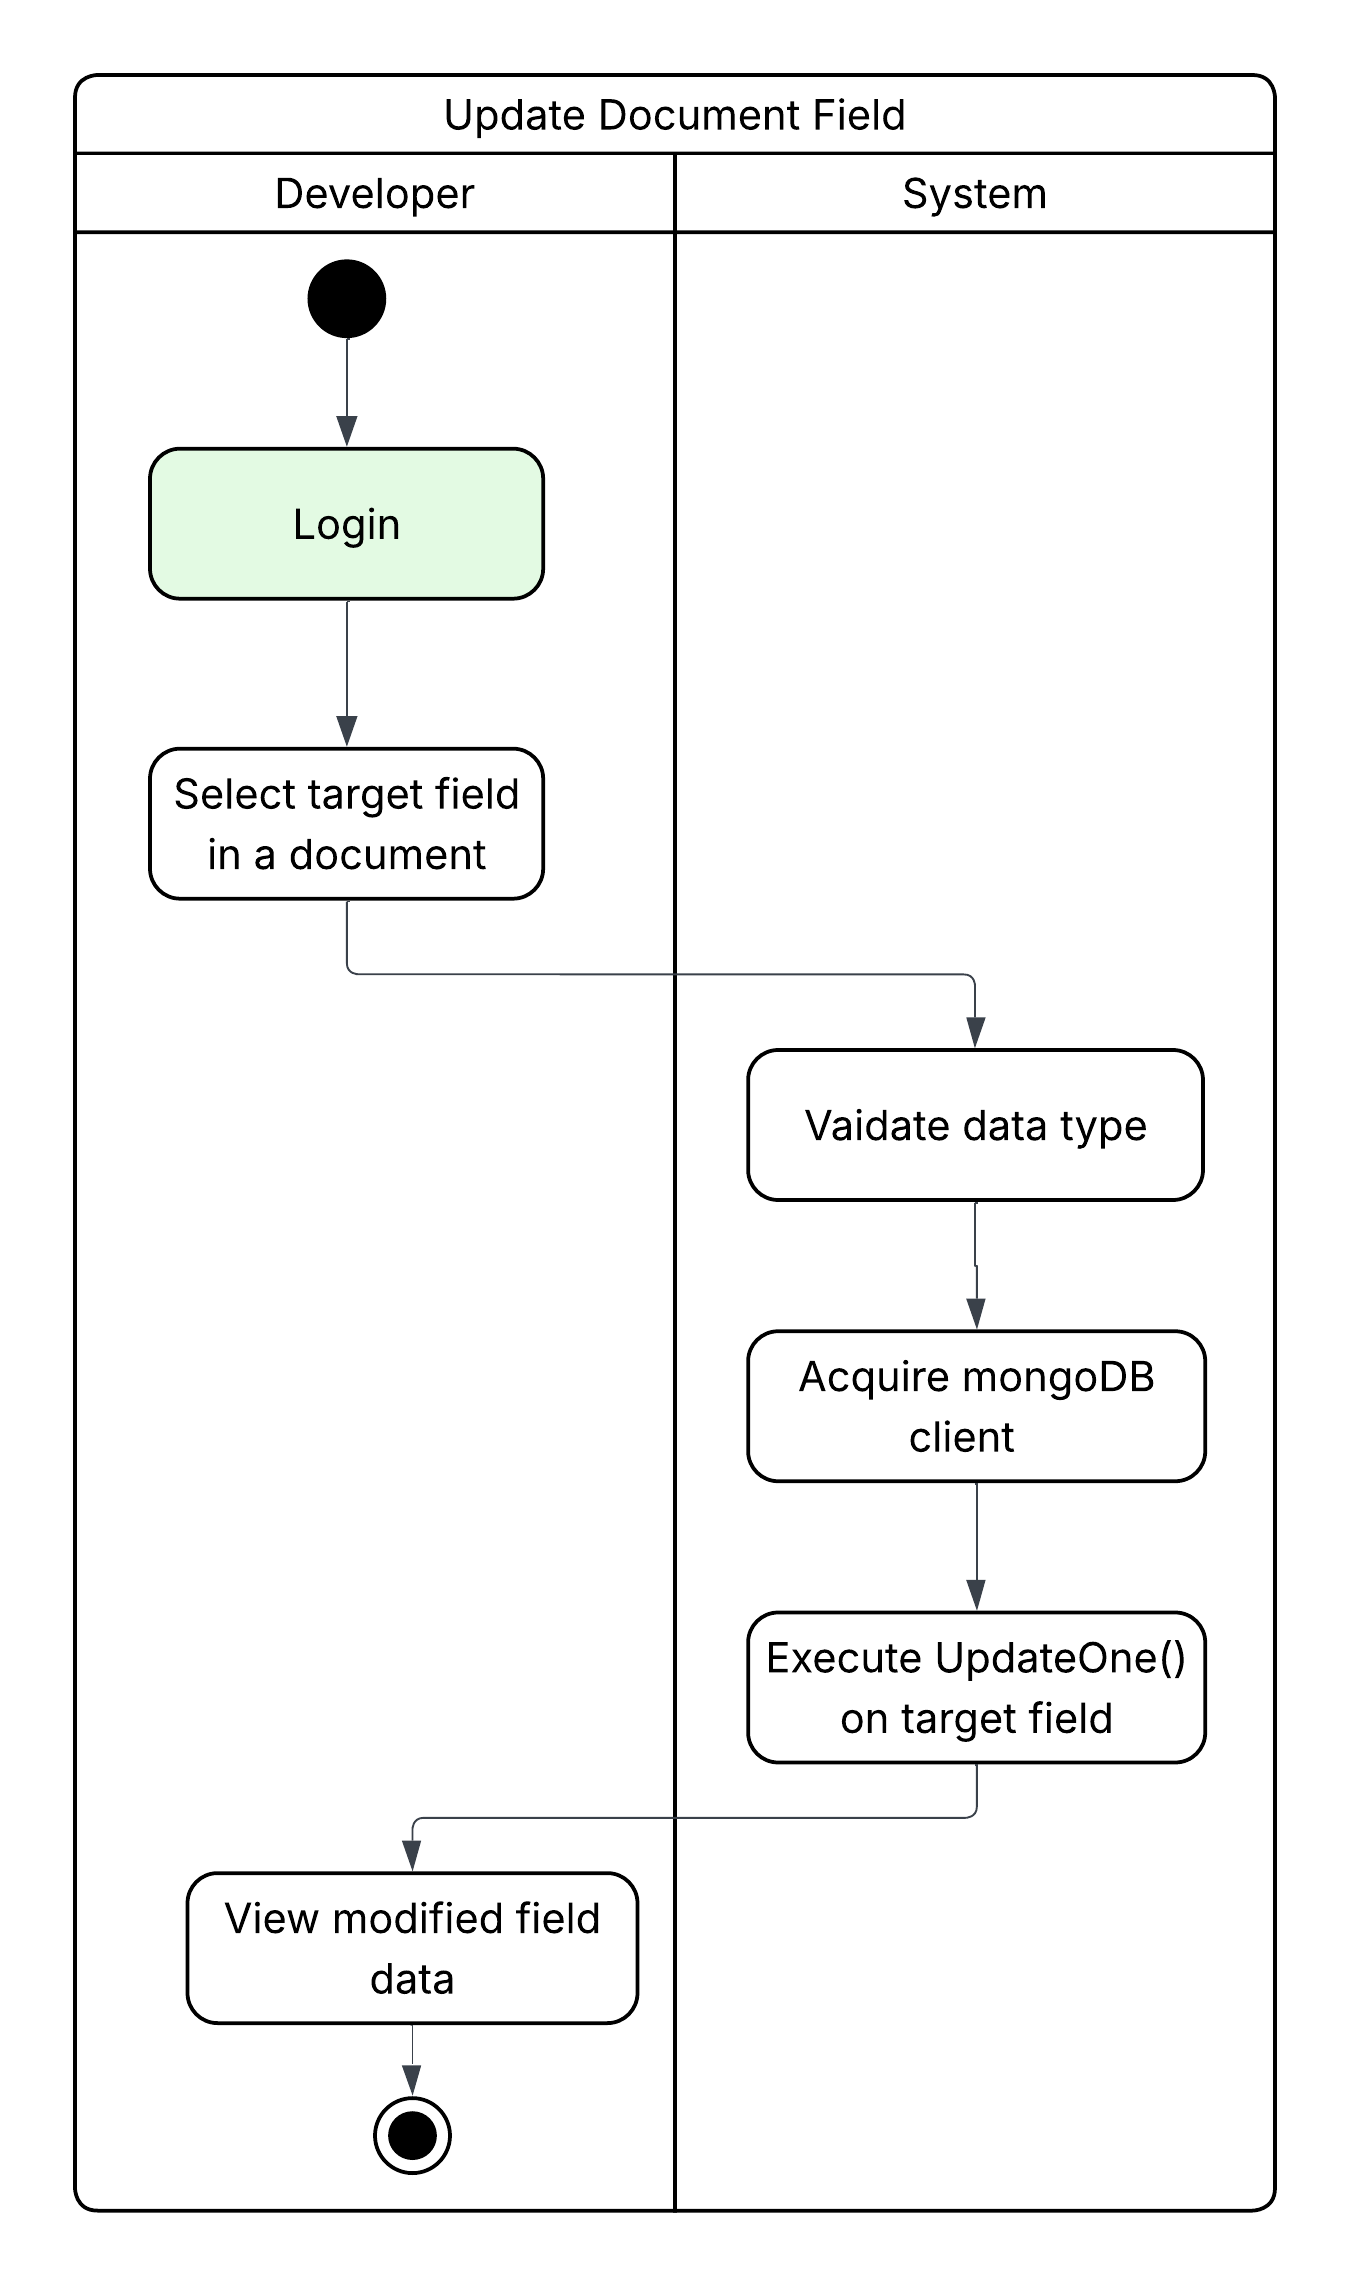
\includegraphics{images/activity/17.Update_a_Field_in_a_Document.png}
        \caption{Update a NoSQL field in a document activity diagram}
        \label{fig:Update_a_Field_in_a_Document}
    \end{figure}

    \begin{figure}[H]
        \centering
        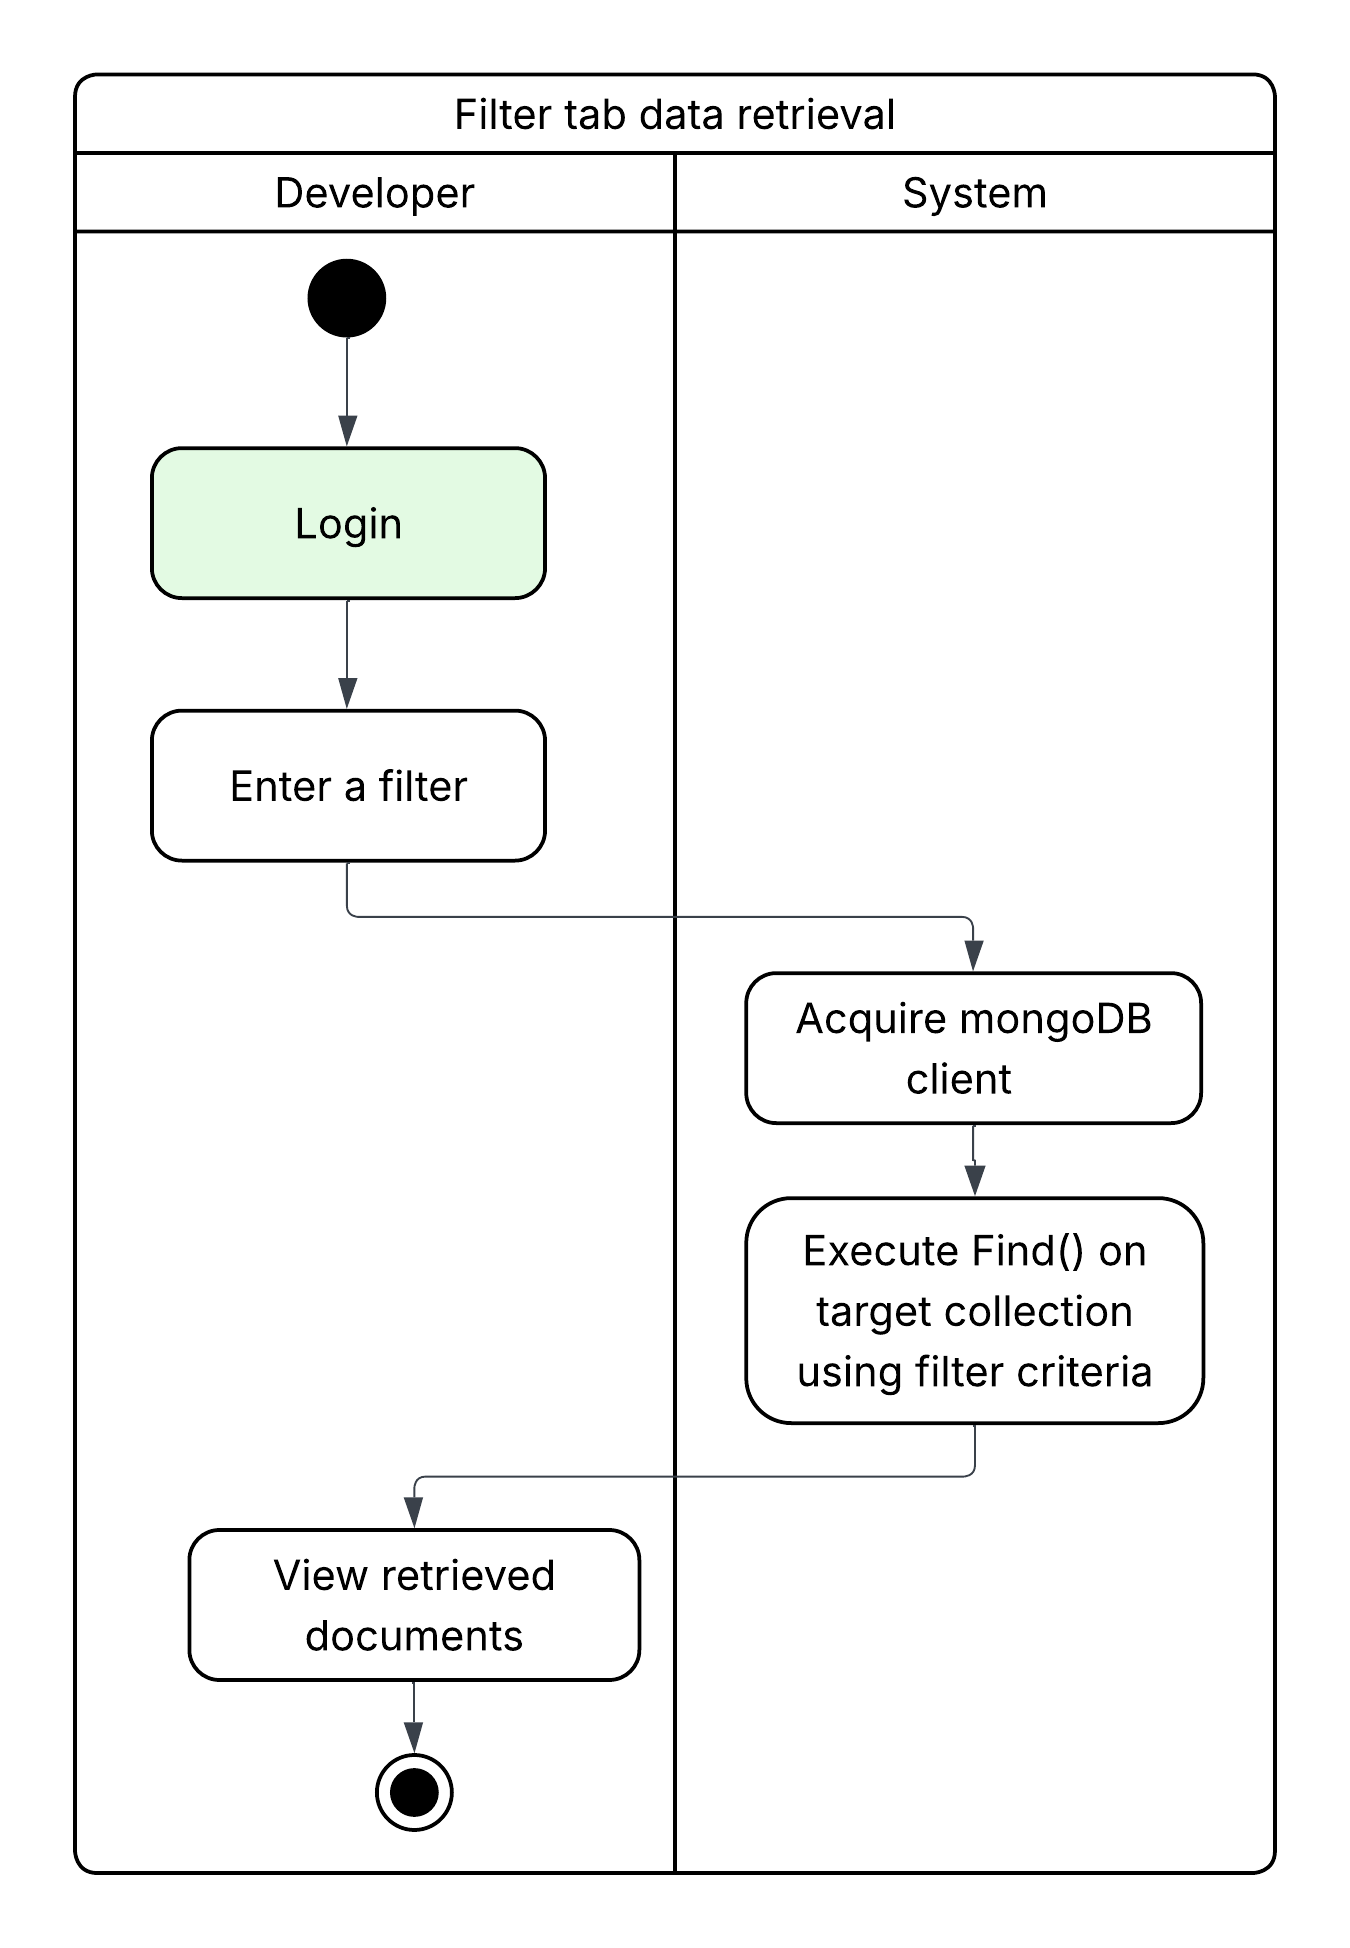
\includegraphics{images/activity/18.Filter_Tab_Data_Retrieval.png}
        \caption{Data retrieval via NoSQL filter activity diagram}
        \label{fig:Filter_Tab_Data_Retrieval}
    \end{figure}

%%%%%%%%%%%%%%%%%%%%%%%%%%%%%%%%%%%%%%%%%
%           Use Case Diagrams           %
%%%%%%%%%%%%%%%%%%%%%%%%%%%%%%%%%%%%%%%%%
\subsection{Use case}
   \begin{figure}[H]
        \centering
        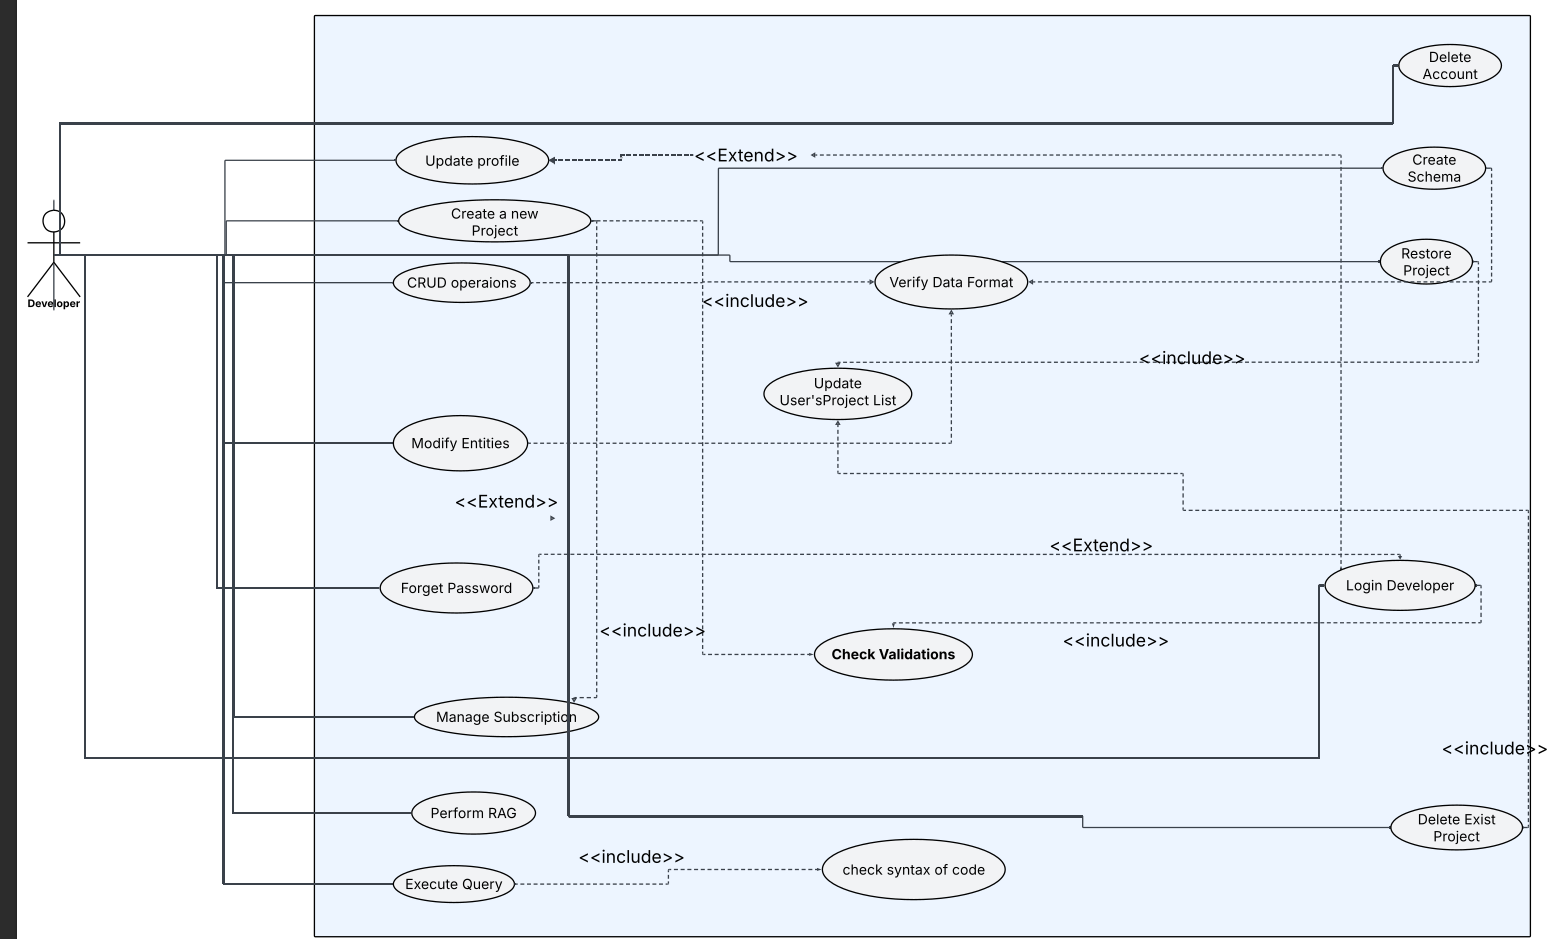
\includegraphics[width=1\linewidth]{images/usecase/usecase.png}
        \caption{Use case diagram}
        \label{fig:usecase_diagram}
    \end{figure}
%%%%%%%%%%%%%%%%%%%%%%%%%%%%%%%%%%%%%%%%%
%           Sequence Diagrams           %
%%%%%%%%%%%%%%%%%%%%%%%%%%%%%%%%%%%%%%%%%
\subsection{Sequence Diagrams}
    \begin{figure}[H]
        \centering
        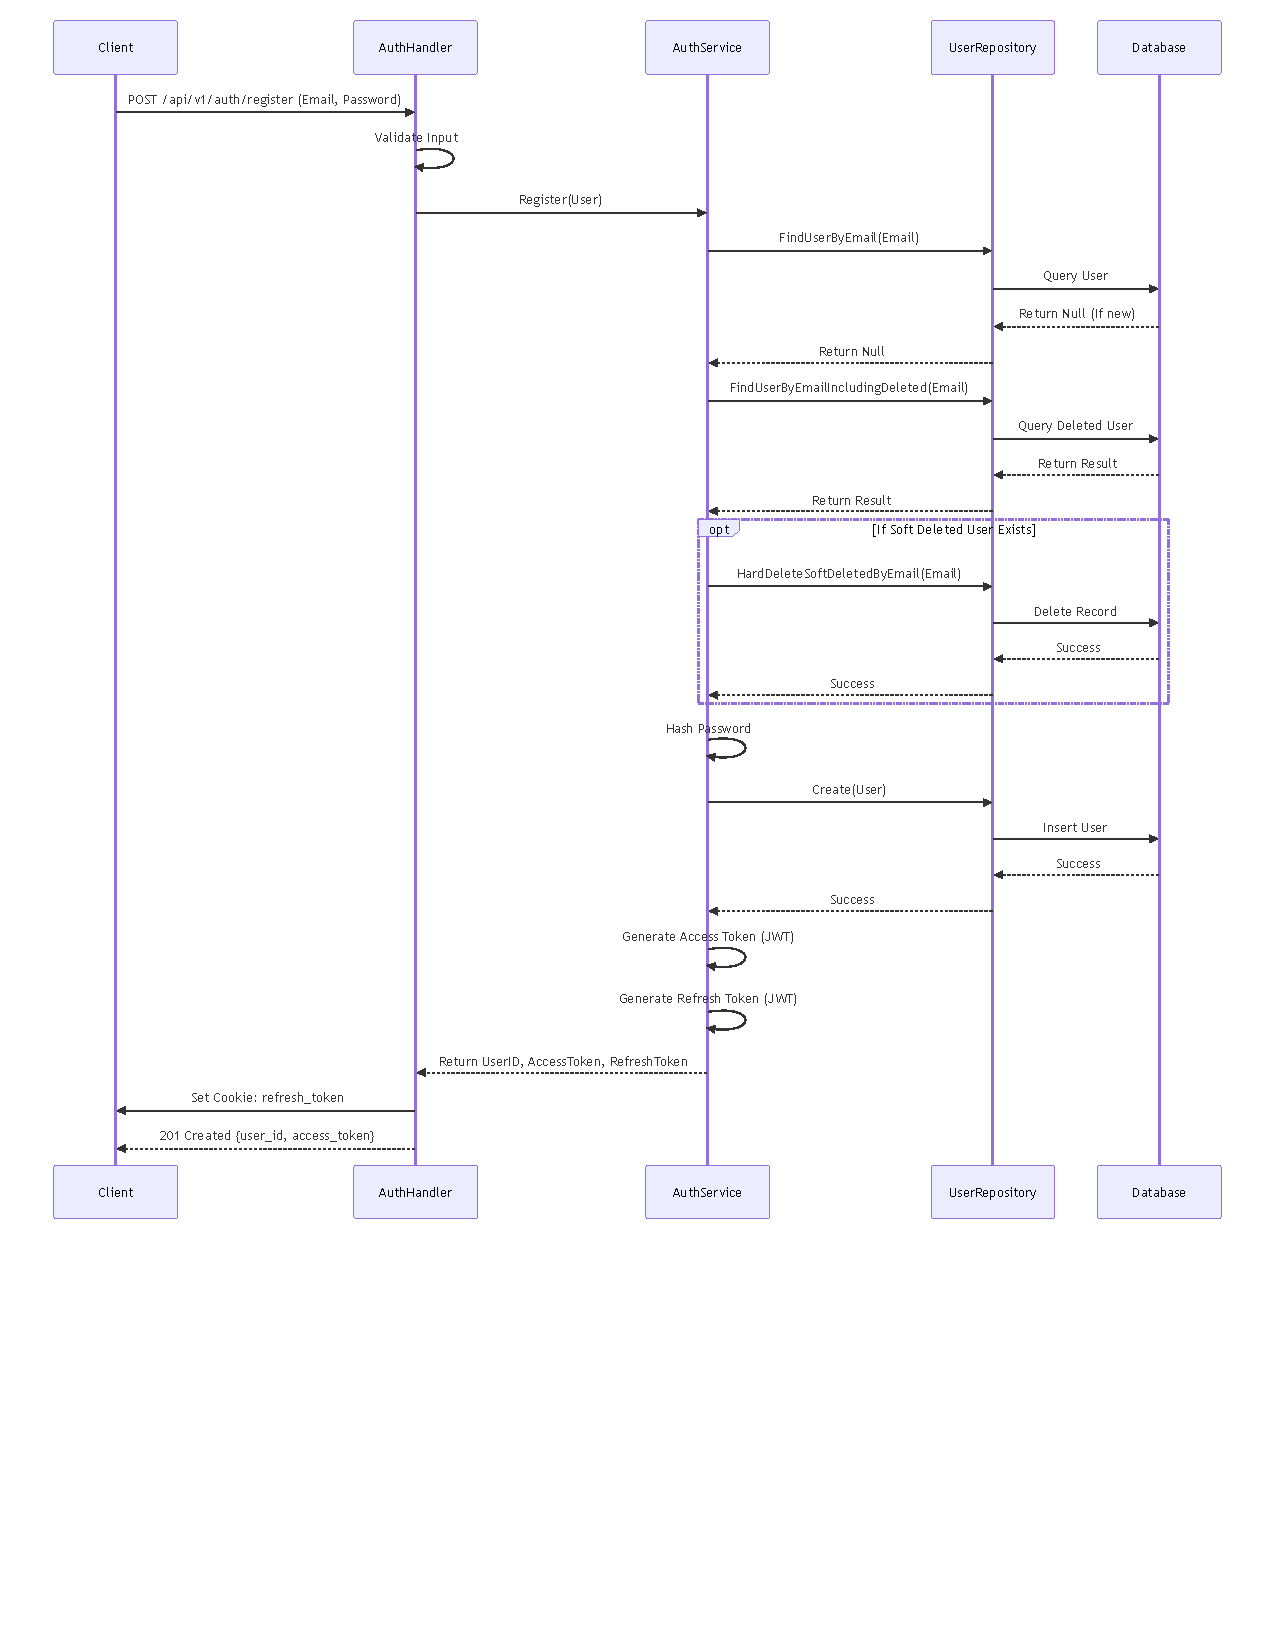
\includegraphics[width=\linewidth,height=0.9\textheight,keepaspectratio]{images/sequence/register_sequence.pdf}
        \caption{Register sequence diagram}
        \label{fig:register_sequence}
    \end{figure}
    
    \begin{figure}[H]
        \centering
        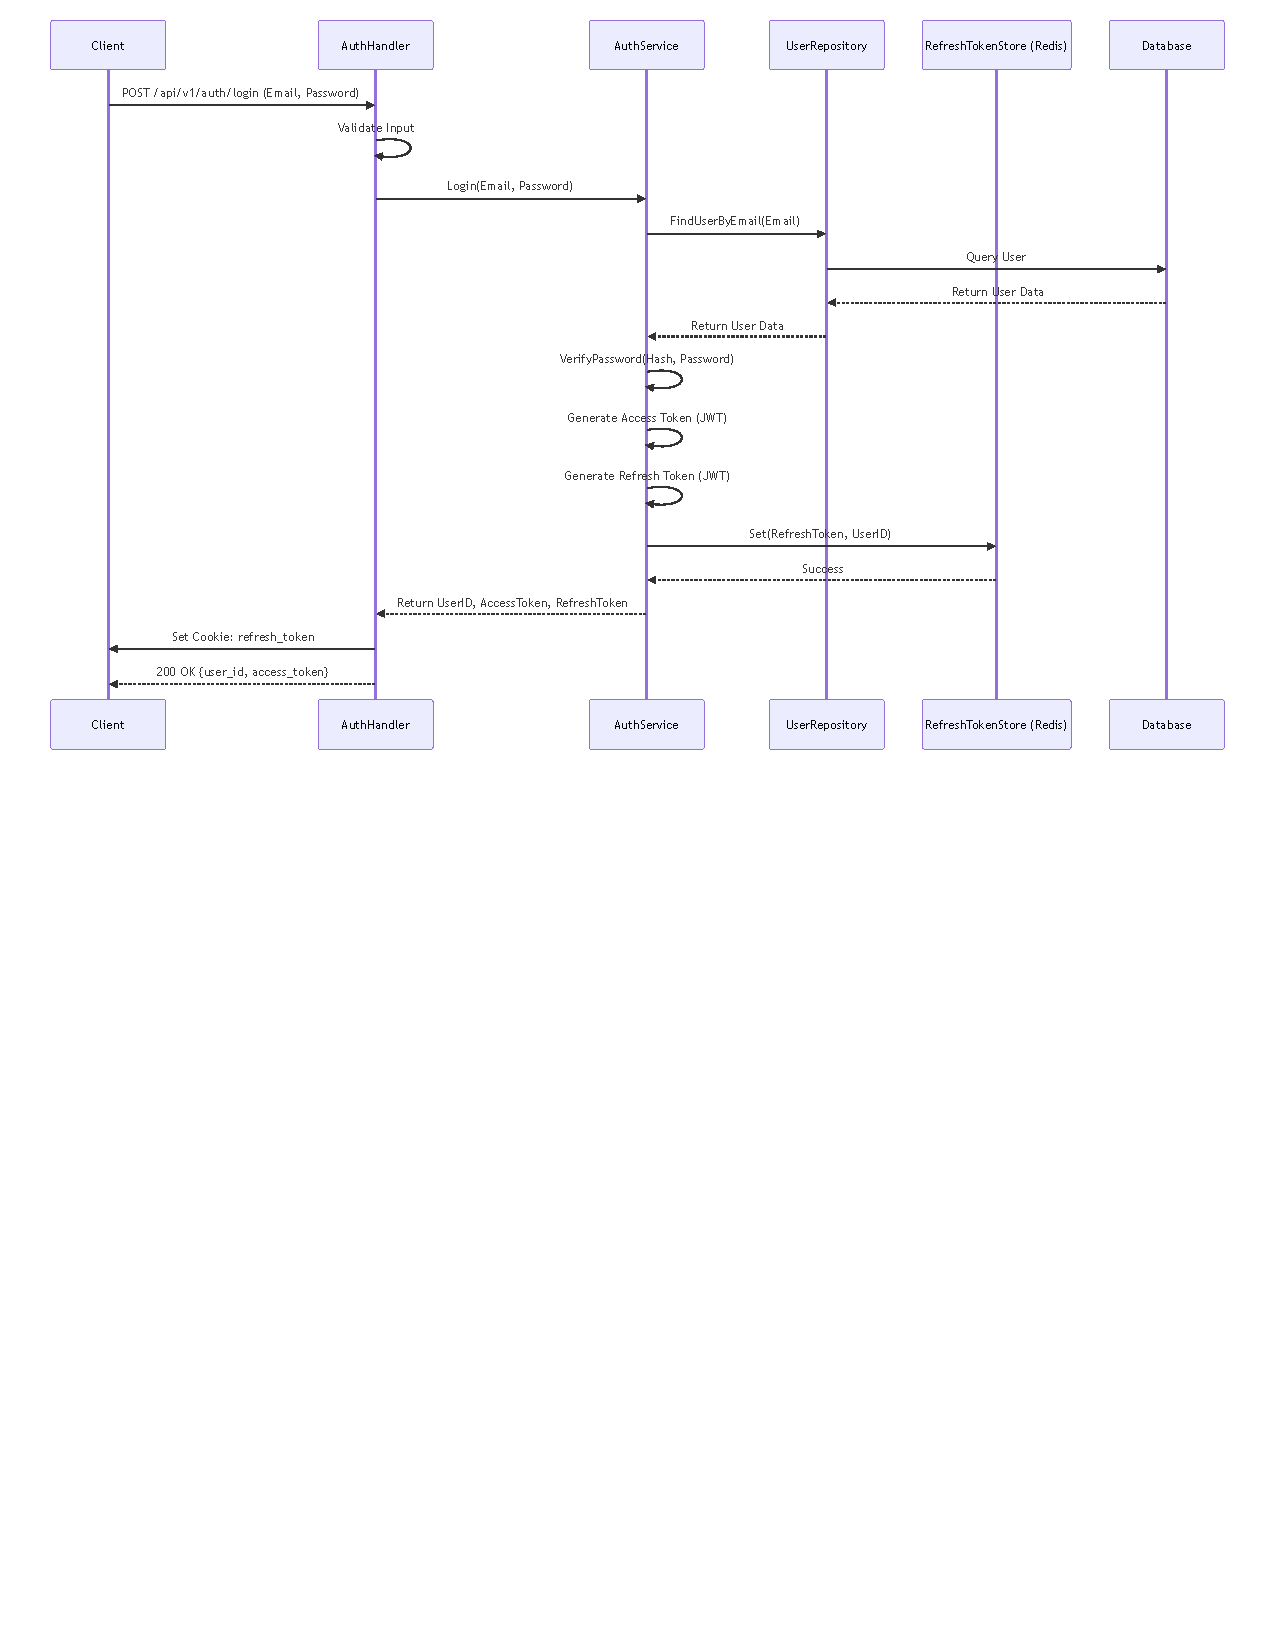
\includegraphics[width=\linewidth,height=0.9\textheight,keepaspectratio]{images/sequence/login.pdf}
        \caption{Login sequence diagram}
        \label{fig:login_sequence}
    \end{figure}
    
    \begin{figure}[H]
        \centering
        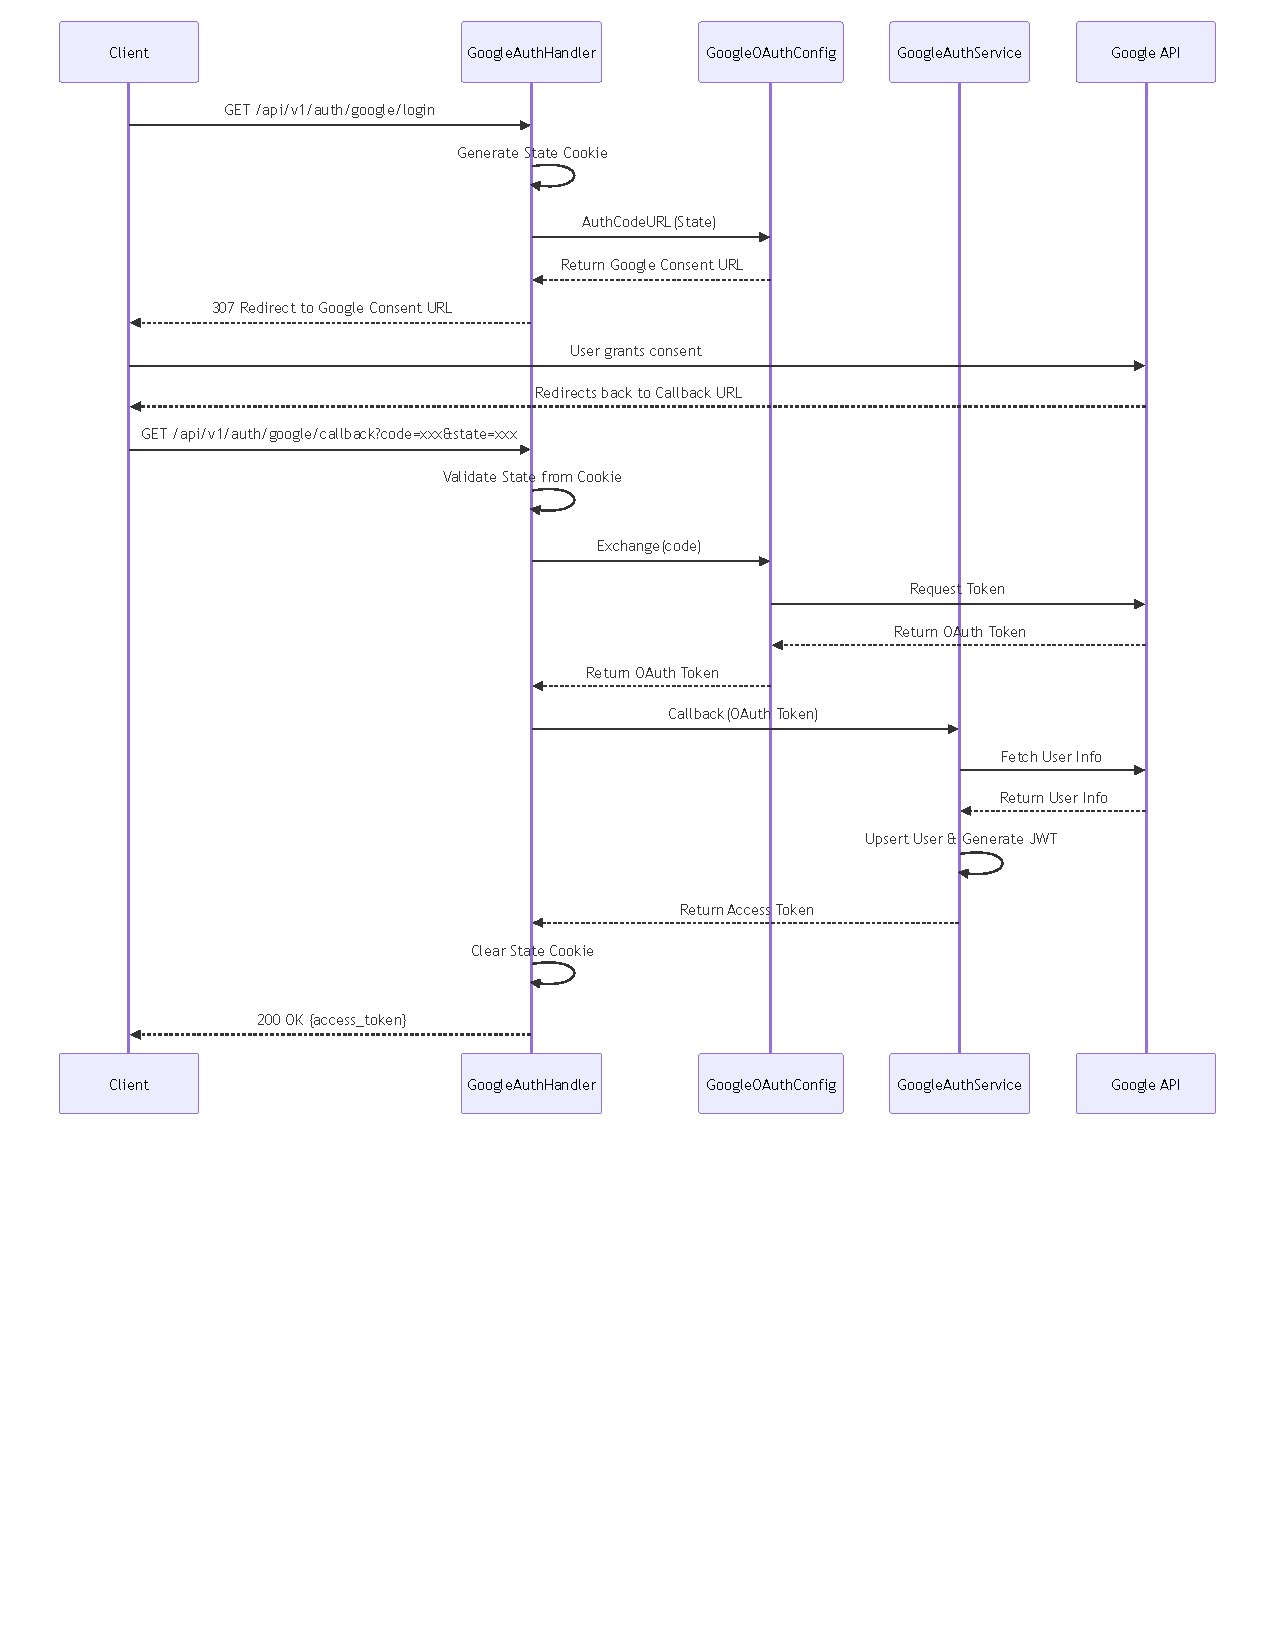
\includegraphics[width=\linewidth,height=0.9\textheight,keepaspectratio]{images/sequence/Oauth_sequence.pdf}
        \caption{Outh sequence diagram}
        \label{fig:oauth_sequence}
    \end{figure}

    \begin{figure}[H]
        \centering
        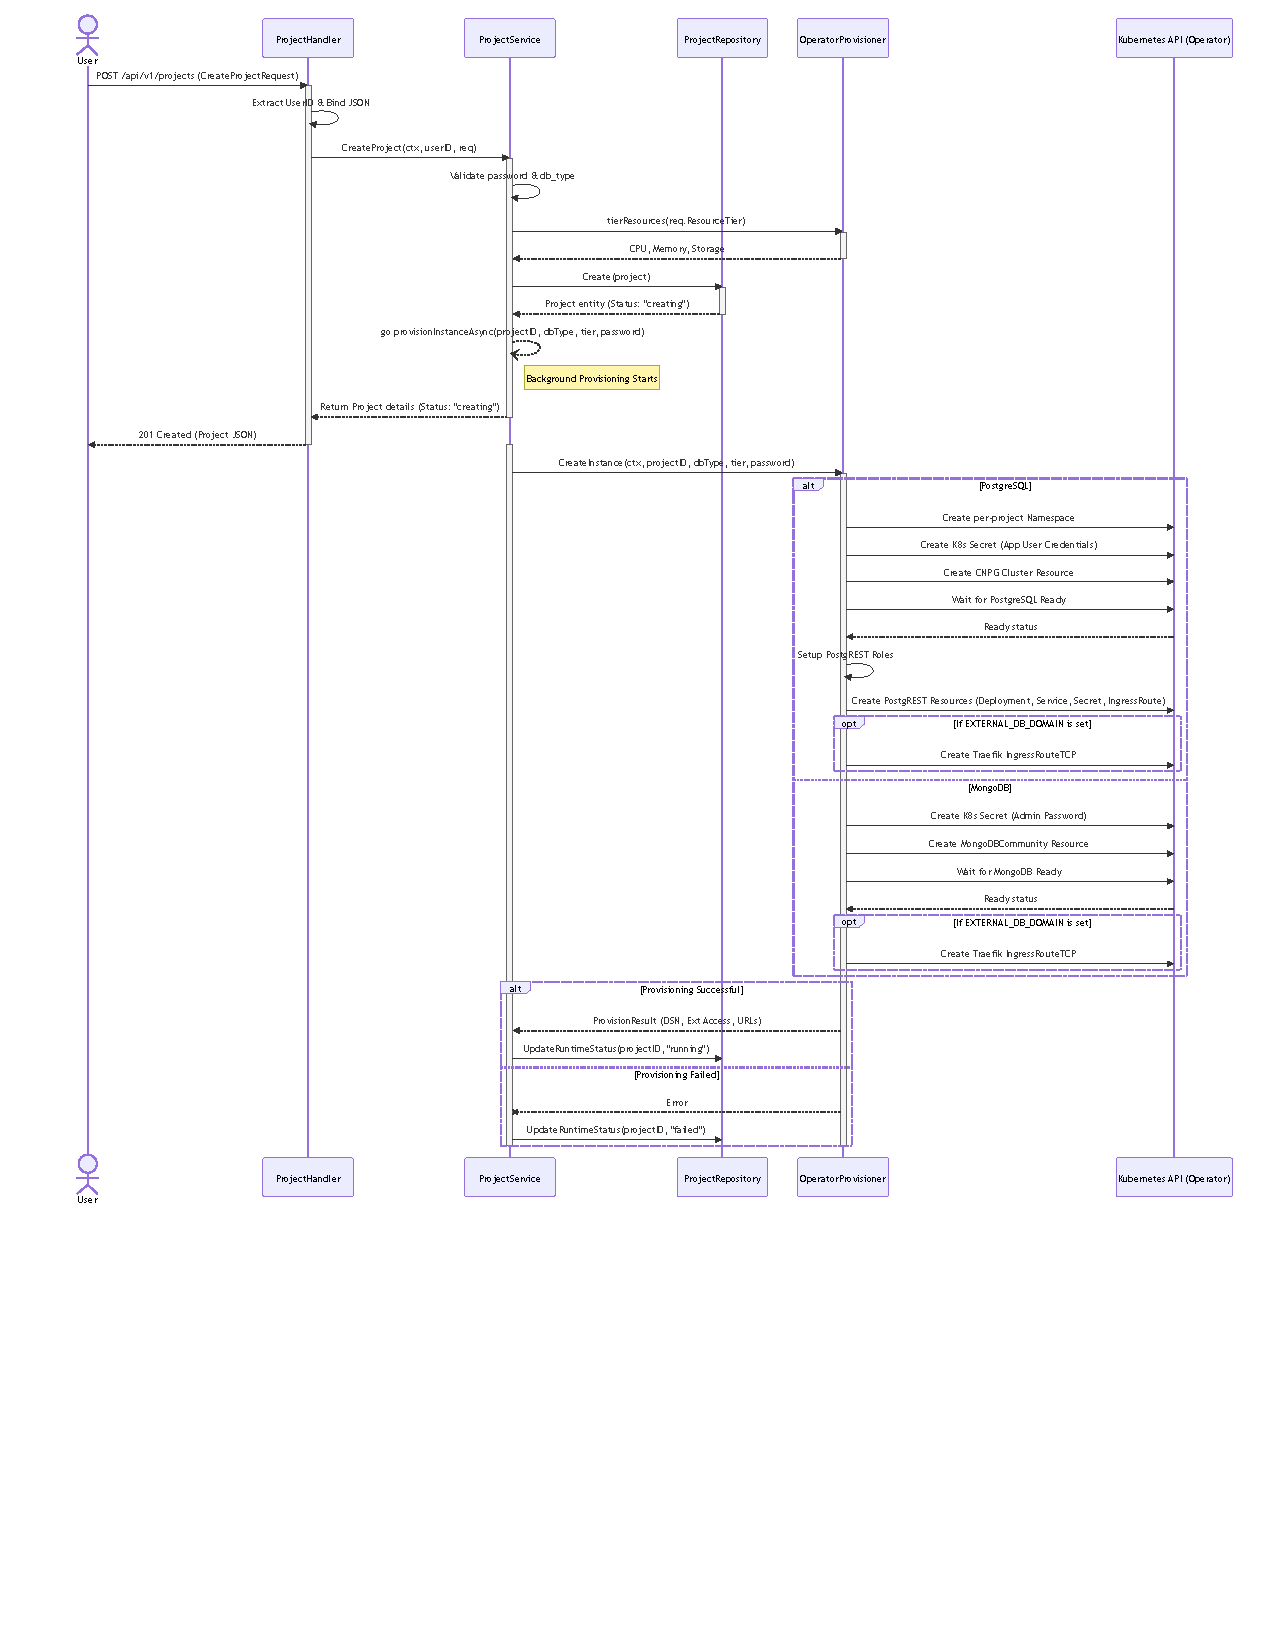
\includegraphics[width=\linewidth,height=0.9\textheight,keepaspectratio]{images/sequence/create_project_seq.pdf}
        \caption{Create project sequence diagram}
        \label{fig:create_project_sequence}
    \end{figure}

    \begin{figure}[H]
        \centering
        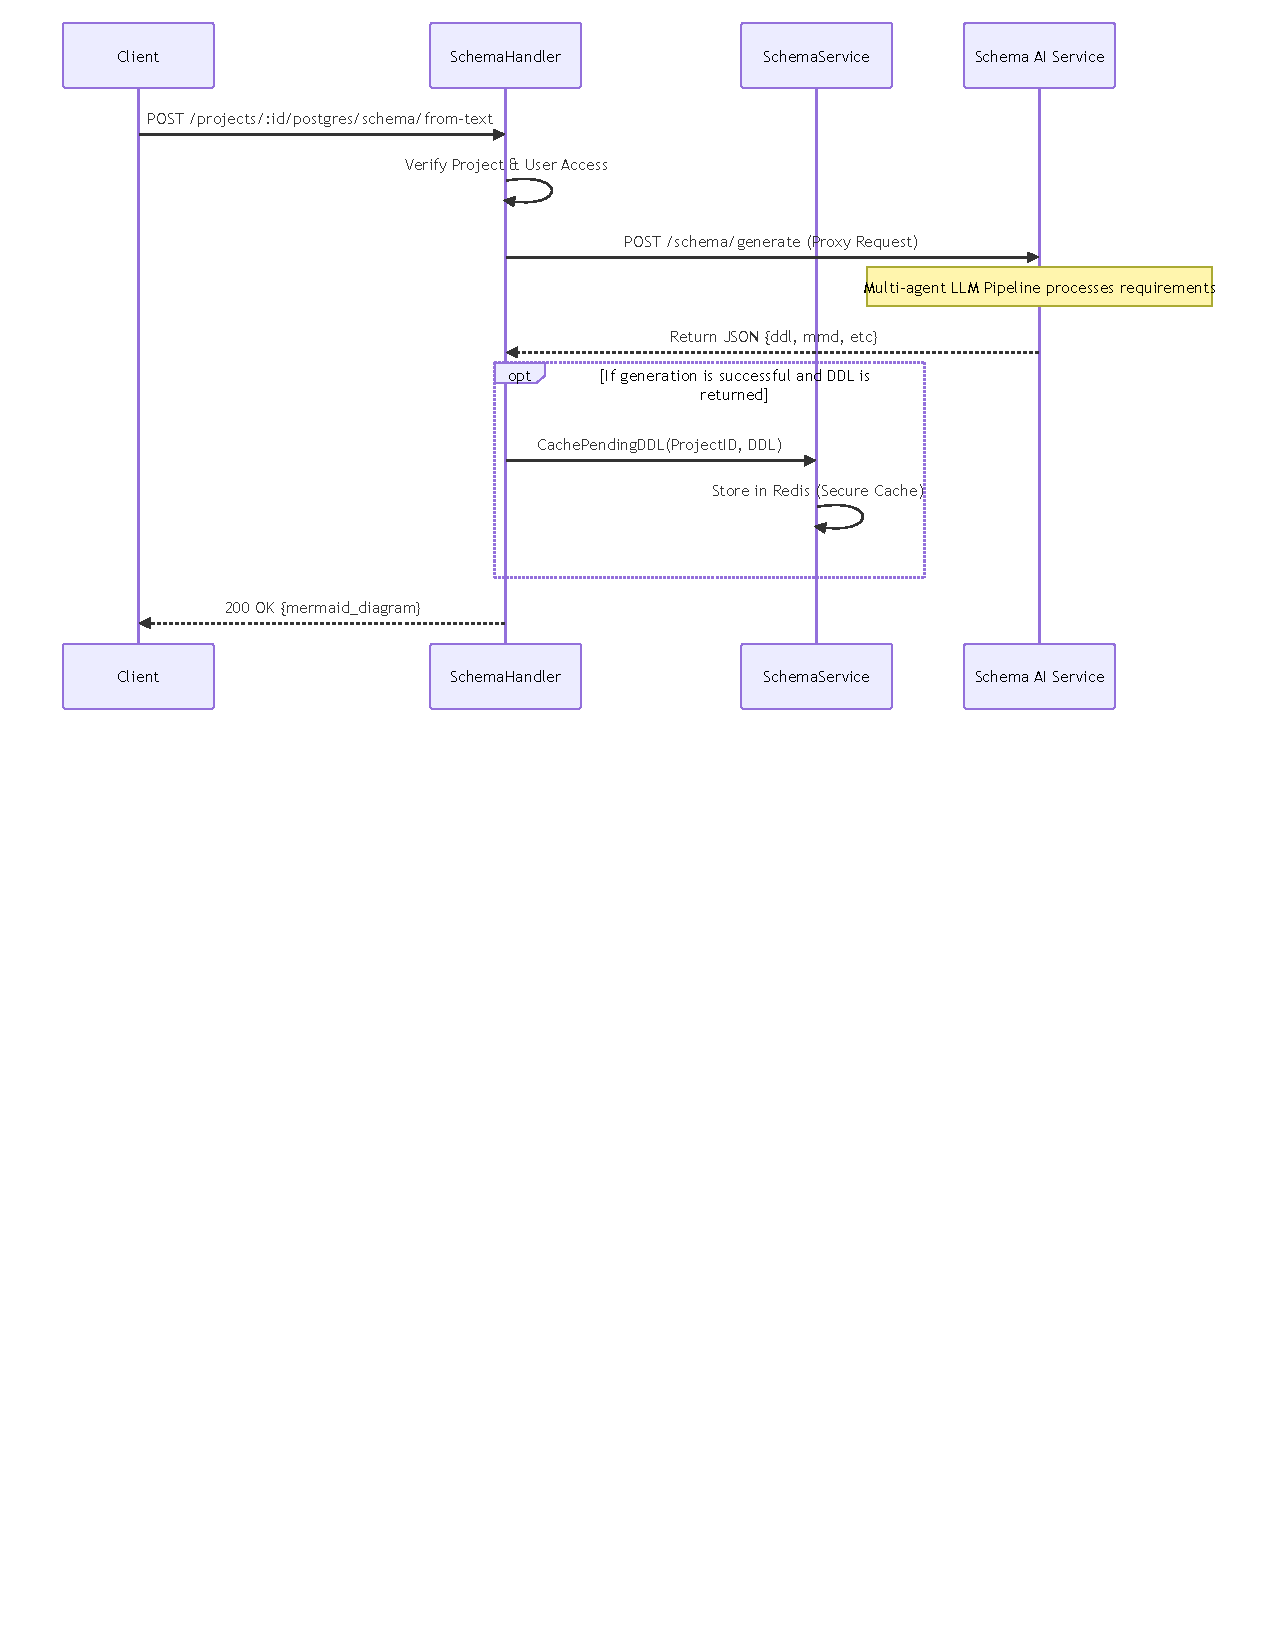
\includegraphics[width=\linewidth,height=0.9\textheight,keepaspectratio]{images/sequence/create_schema_seq.pdf}
        \caption{Create schema sequence diagram}
        \label{fig:create_schema_sequence}
    \end{figure}
    
   \begin{figure}[H]
        \centering
        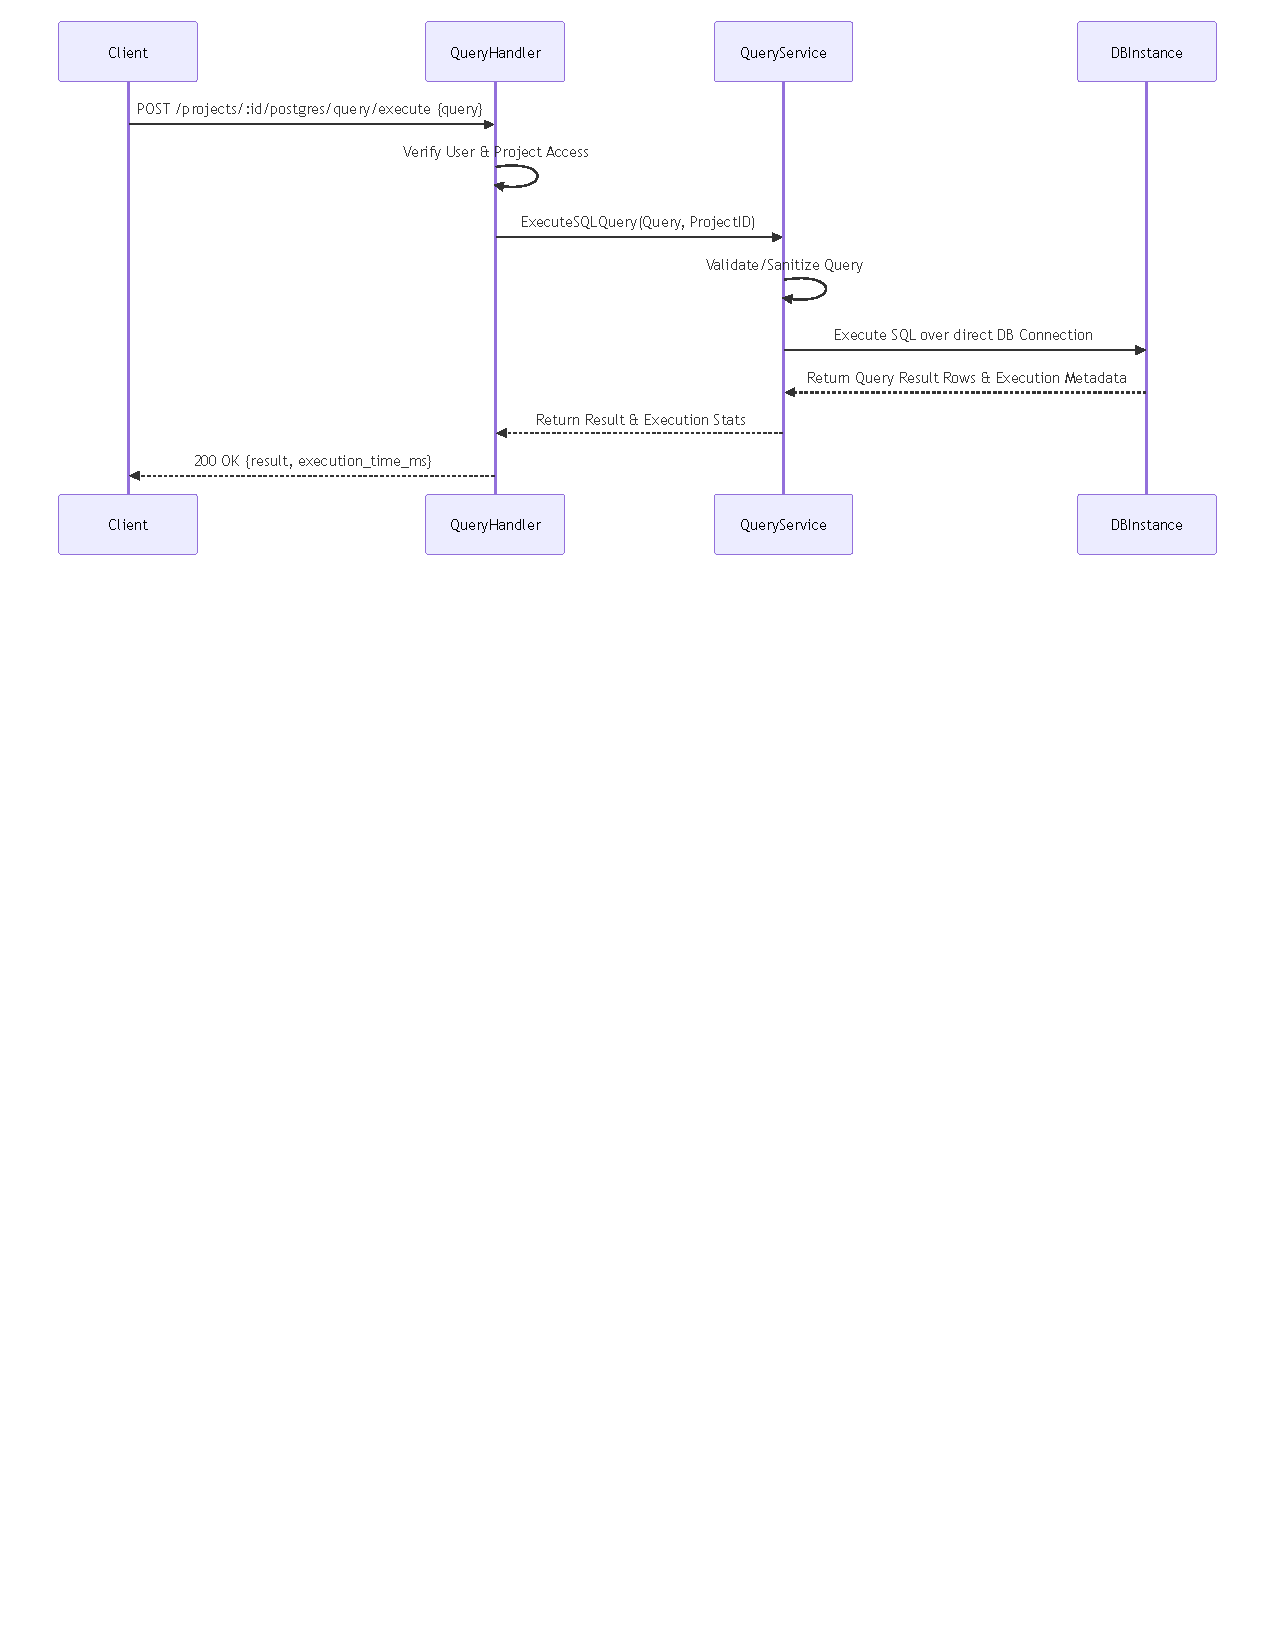
\includegraphics[width=\linewidth,height=0.9\textheight,keepaspectratio]{images/sequence/execute_query_sequence.pdf}
        \caption{Execute SQL query sequence diagram}
        \label{fig:execute_query_sequence}
    \end{figure}
    
    \begin{figure}[H]
        \centering
        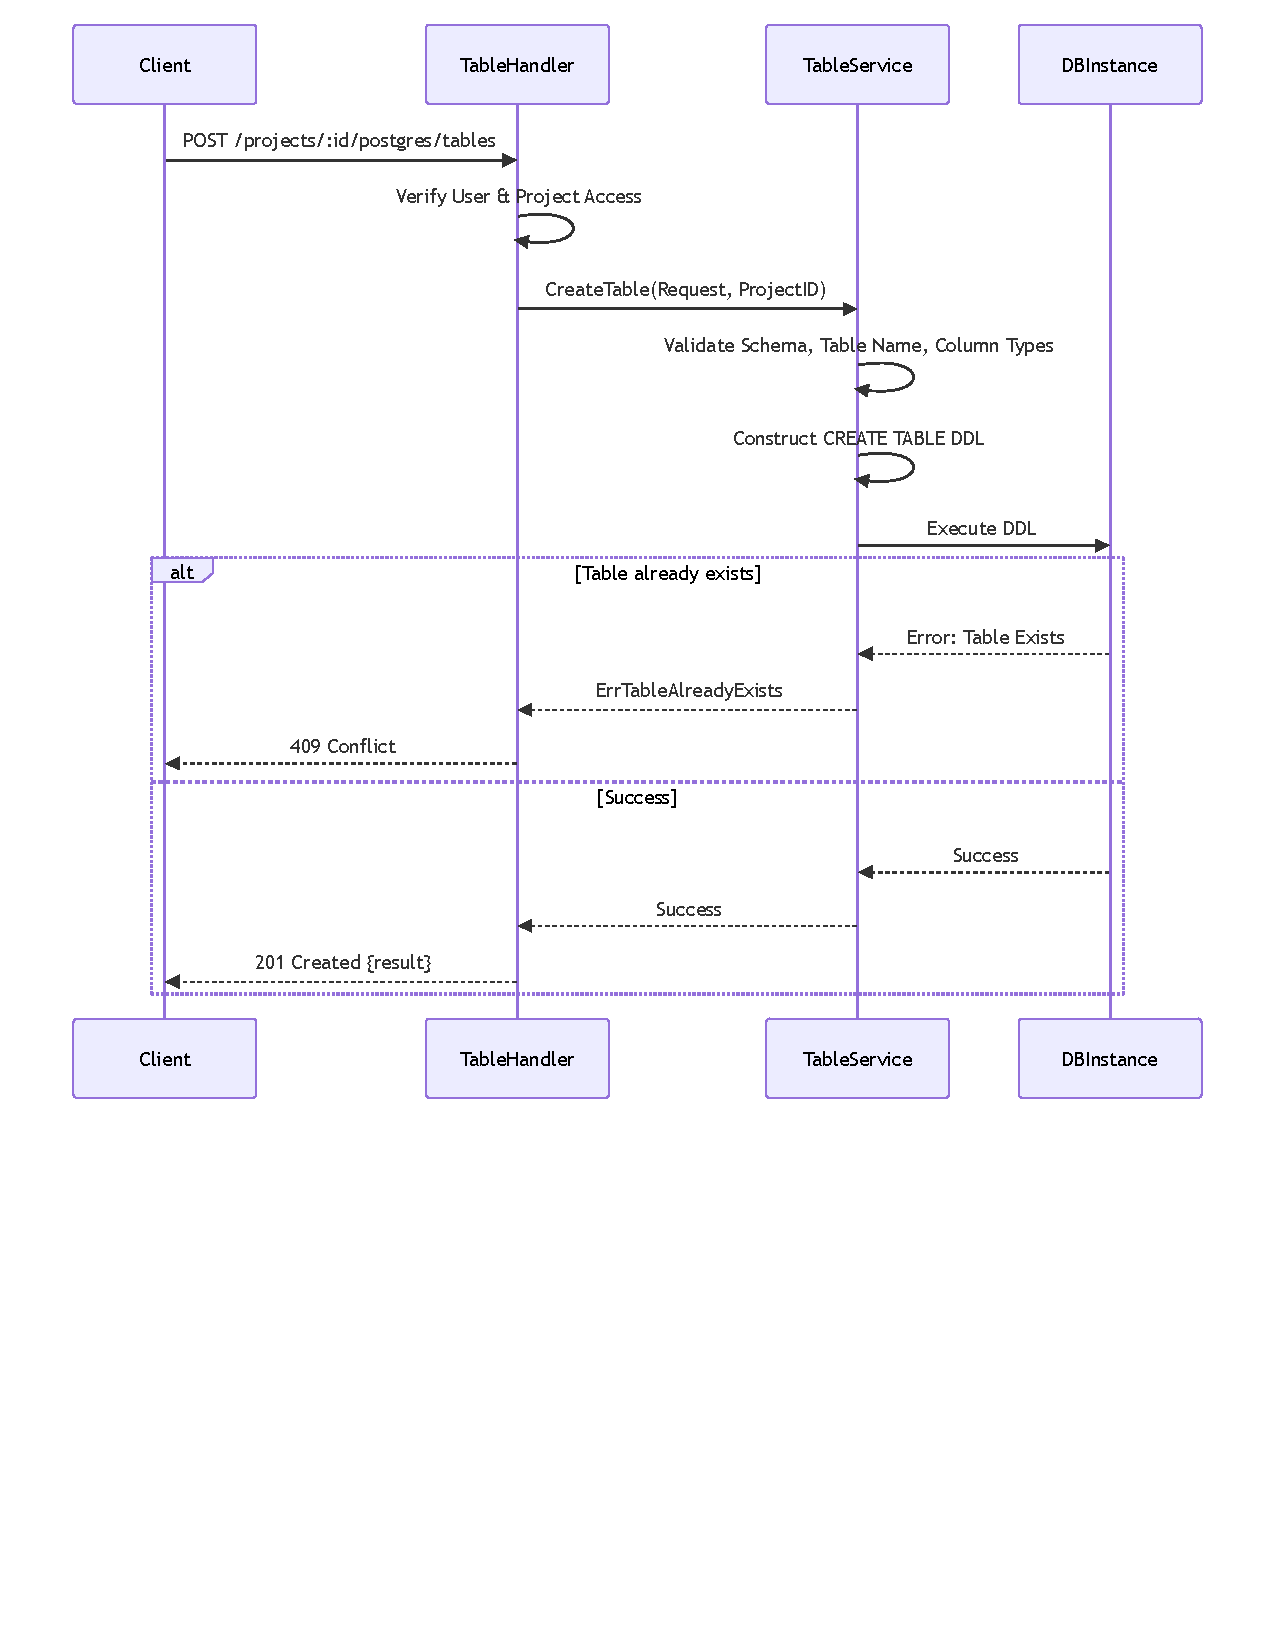
\includegraphics[width=\linewidth,height=0.9\textheight,keepaspectratio]{images/sequence/create_table.pdf}
        \caption{Create table sequence diagram}
        \label{fig:create_table_sequence}
    \end{figure}

    \begin{figure}[H]
        \centering
        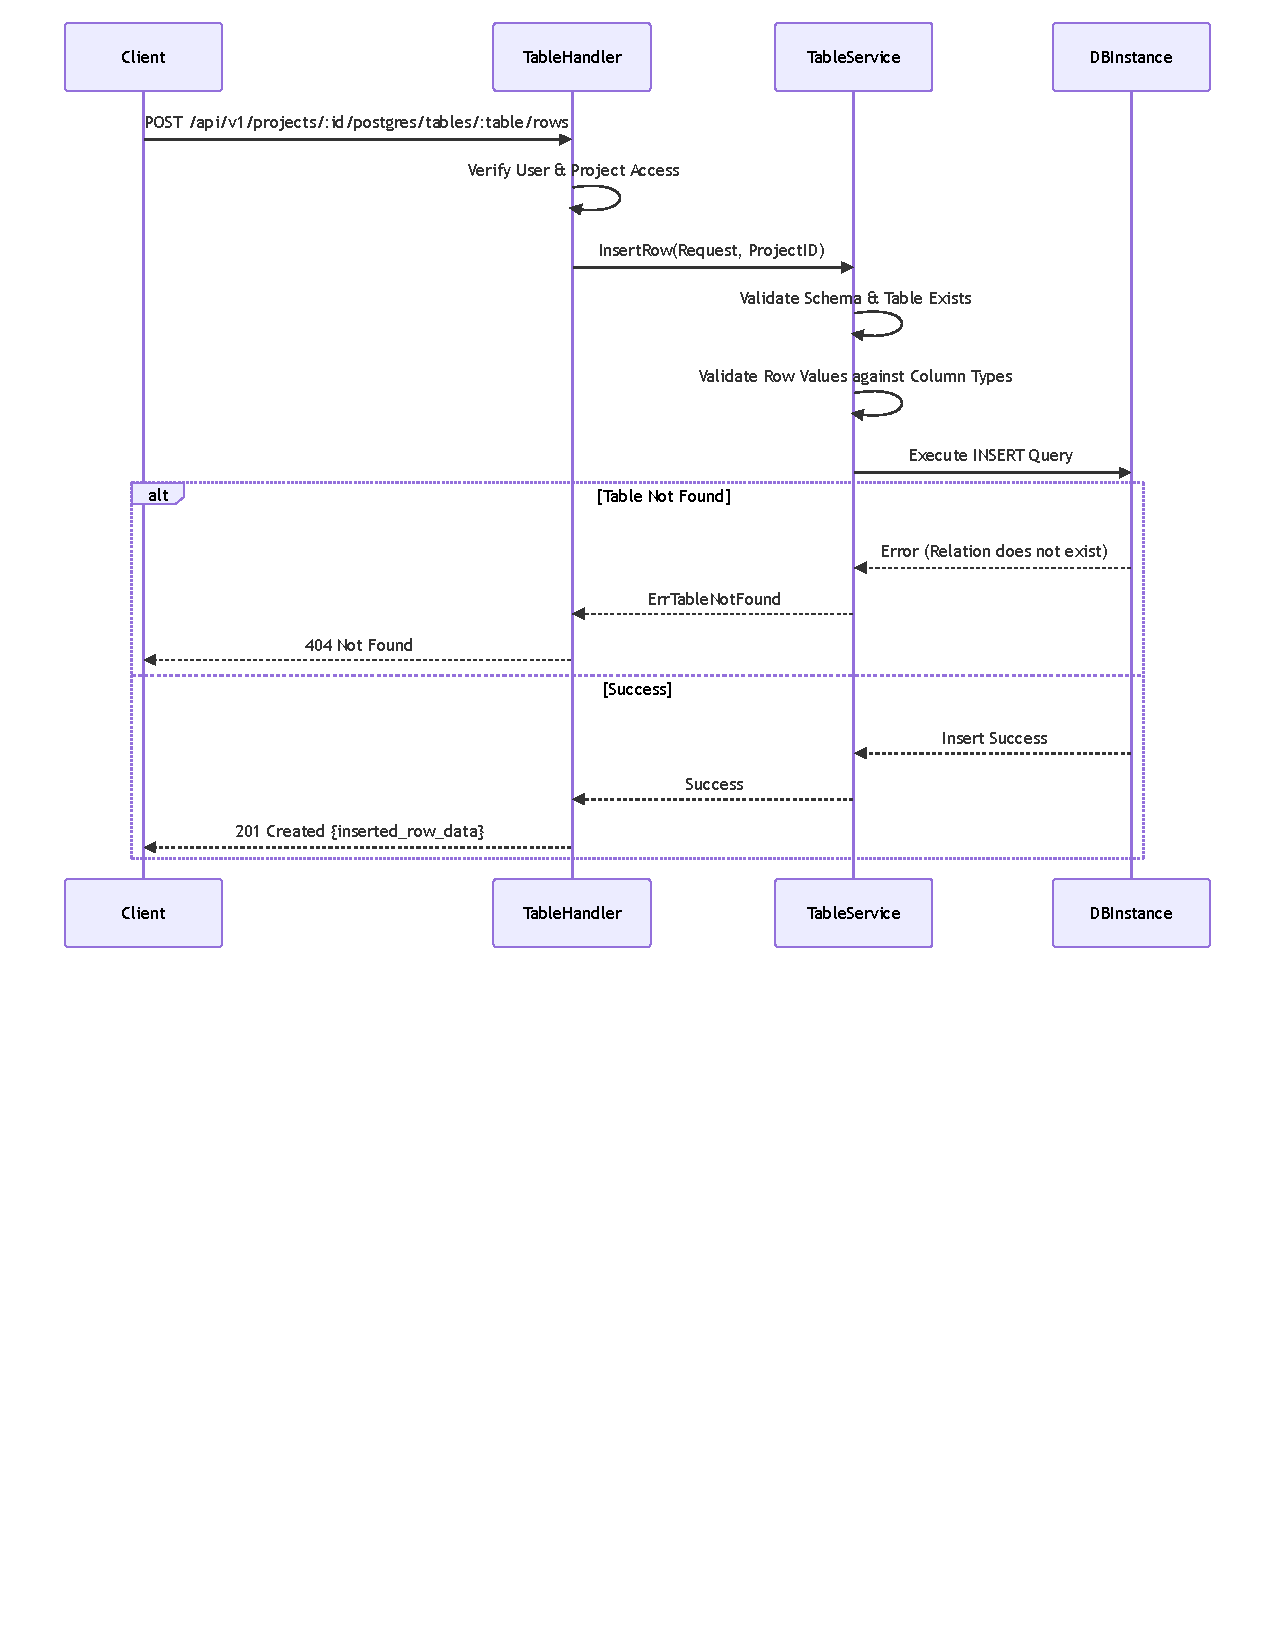
\includegraphics[width=\linewidth,height=0.9\textheight,keepaspectratio]{images/sequence/modify_data_sql_sequence.pdf}
        \caption{Modify data (SQL) sequence diagram}
        \label{fig:modify_data_sql_sequence}
    \end{figure}

    \begin{figure}[H]
        \centering
        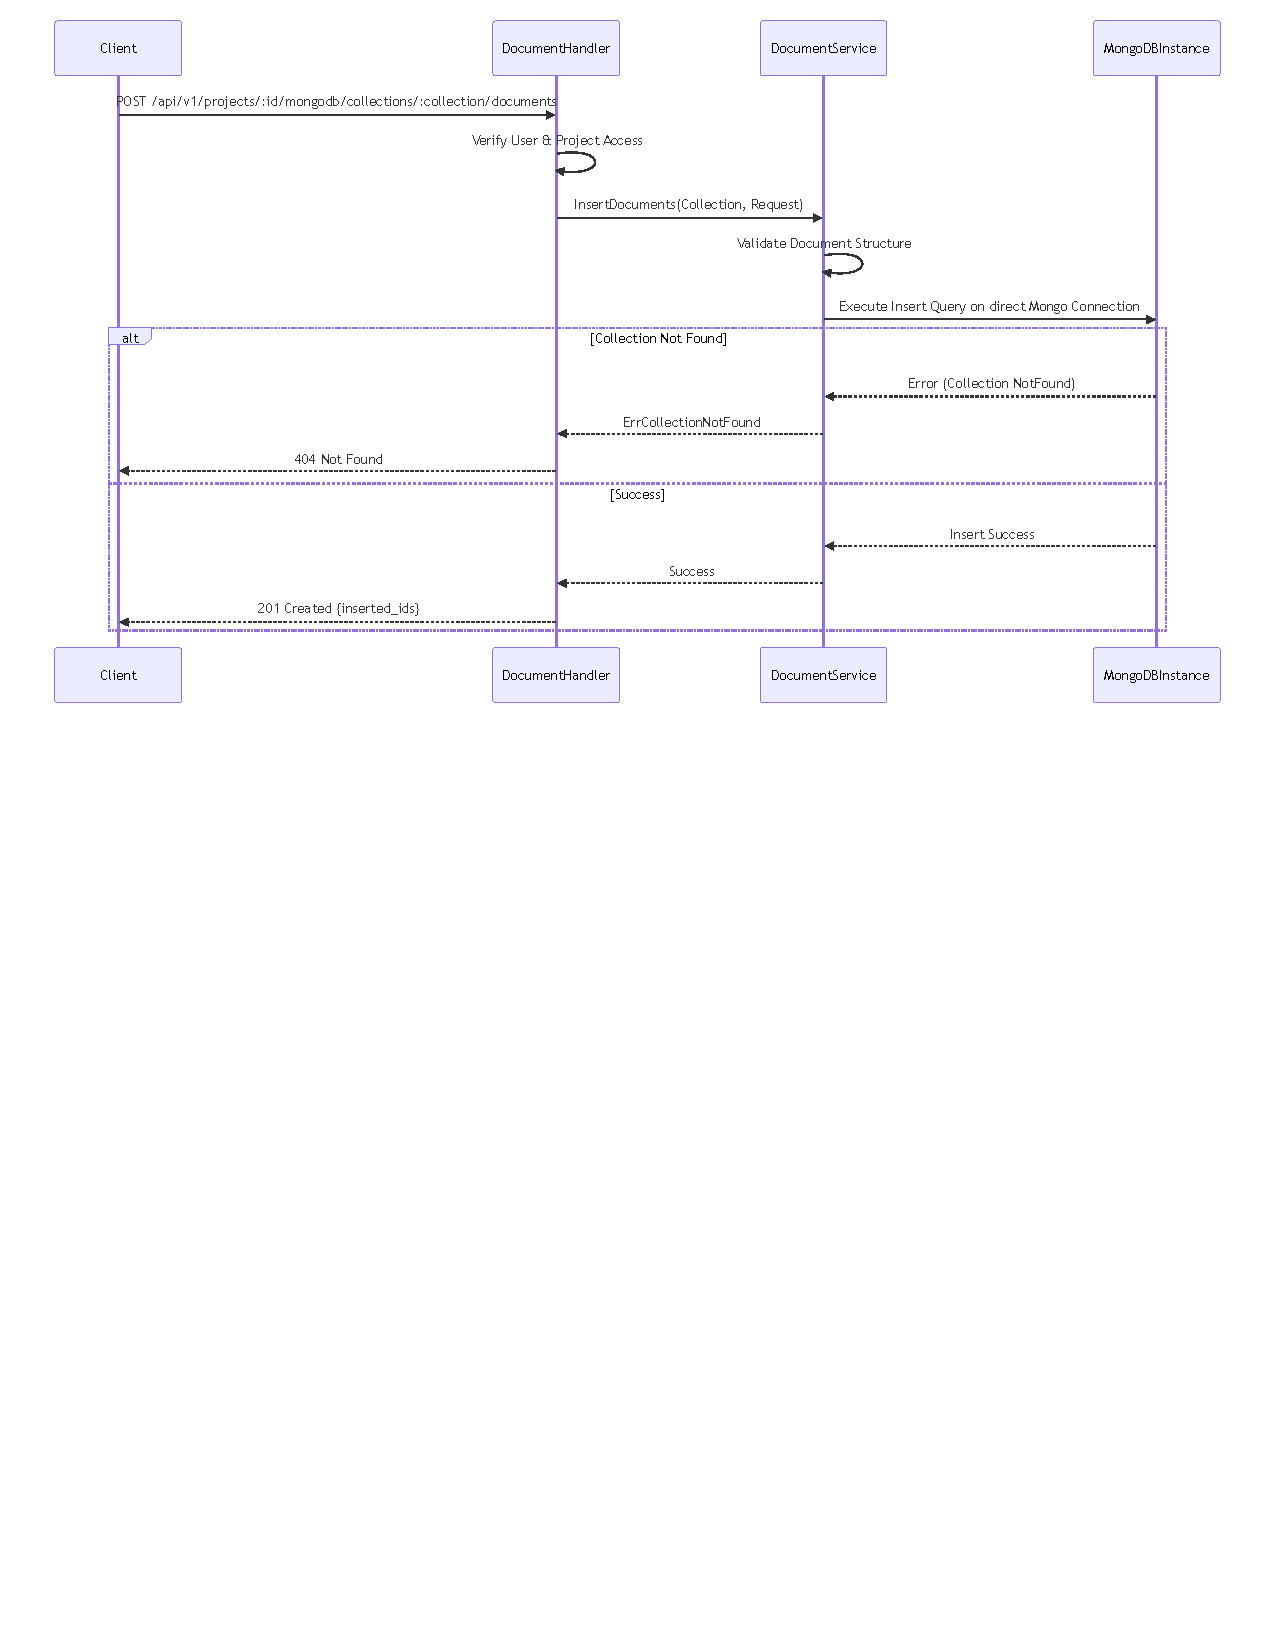
\includegraphics[width=\linewidth,height=0.9\textheight,keepaspectratio]{images/sequence/modify_entity_nosql_sequence.pdf}
        \caption{Modify entity (NOSQL) sequence diagram}
        \label{fig:modify_entity_nosql_sequence}
    \end{figure}

%%%%%%%%%%%%%%%%%%%%%%%%%%%%%%%%%%%%%%%%%%%%%%%%%%%%%%%%%%%%%








%%%%%%%%%%%%%%%%%%%%%%%%%%%%%%%%%%%%%%%%%%%%%%%%%%%%%%%%%%%%%
    
    \begin{figure}[H]
        \centering
        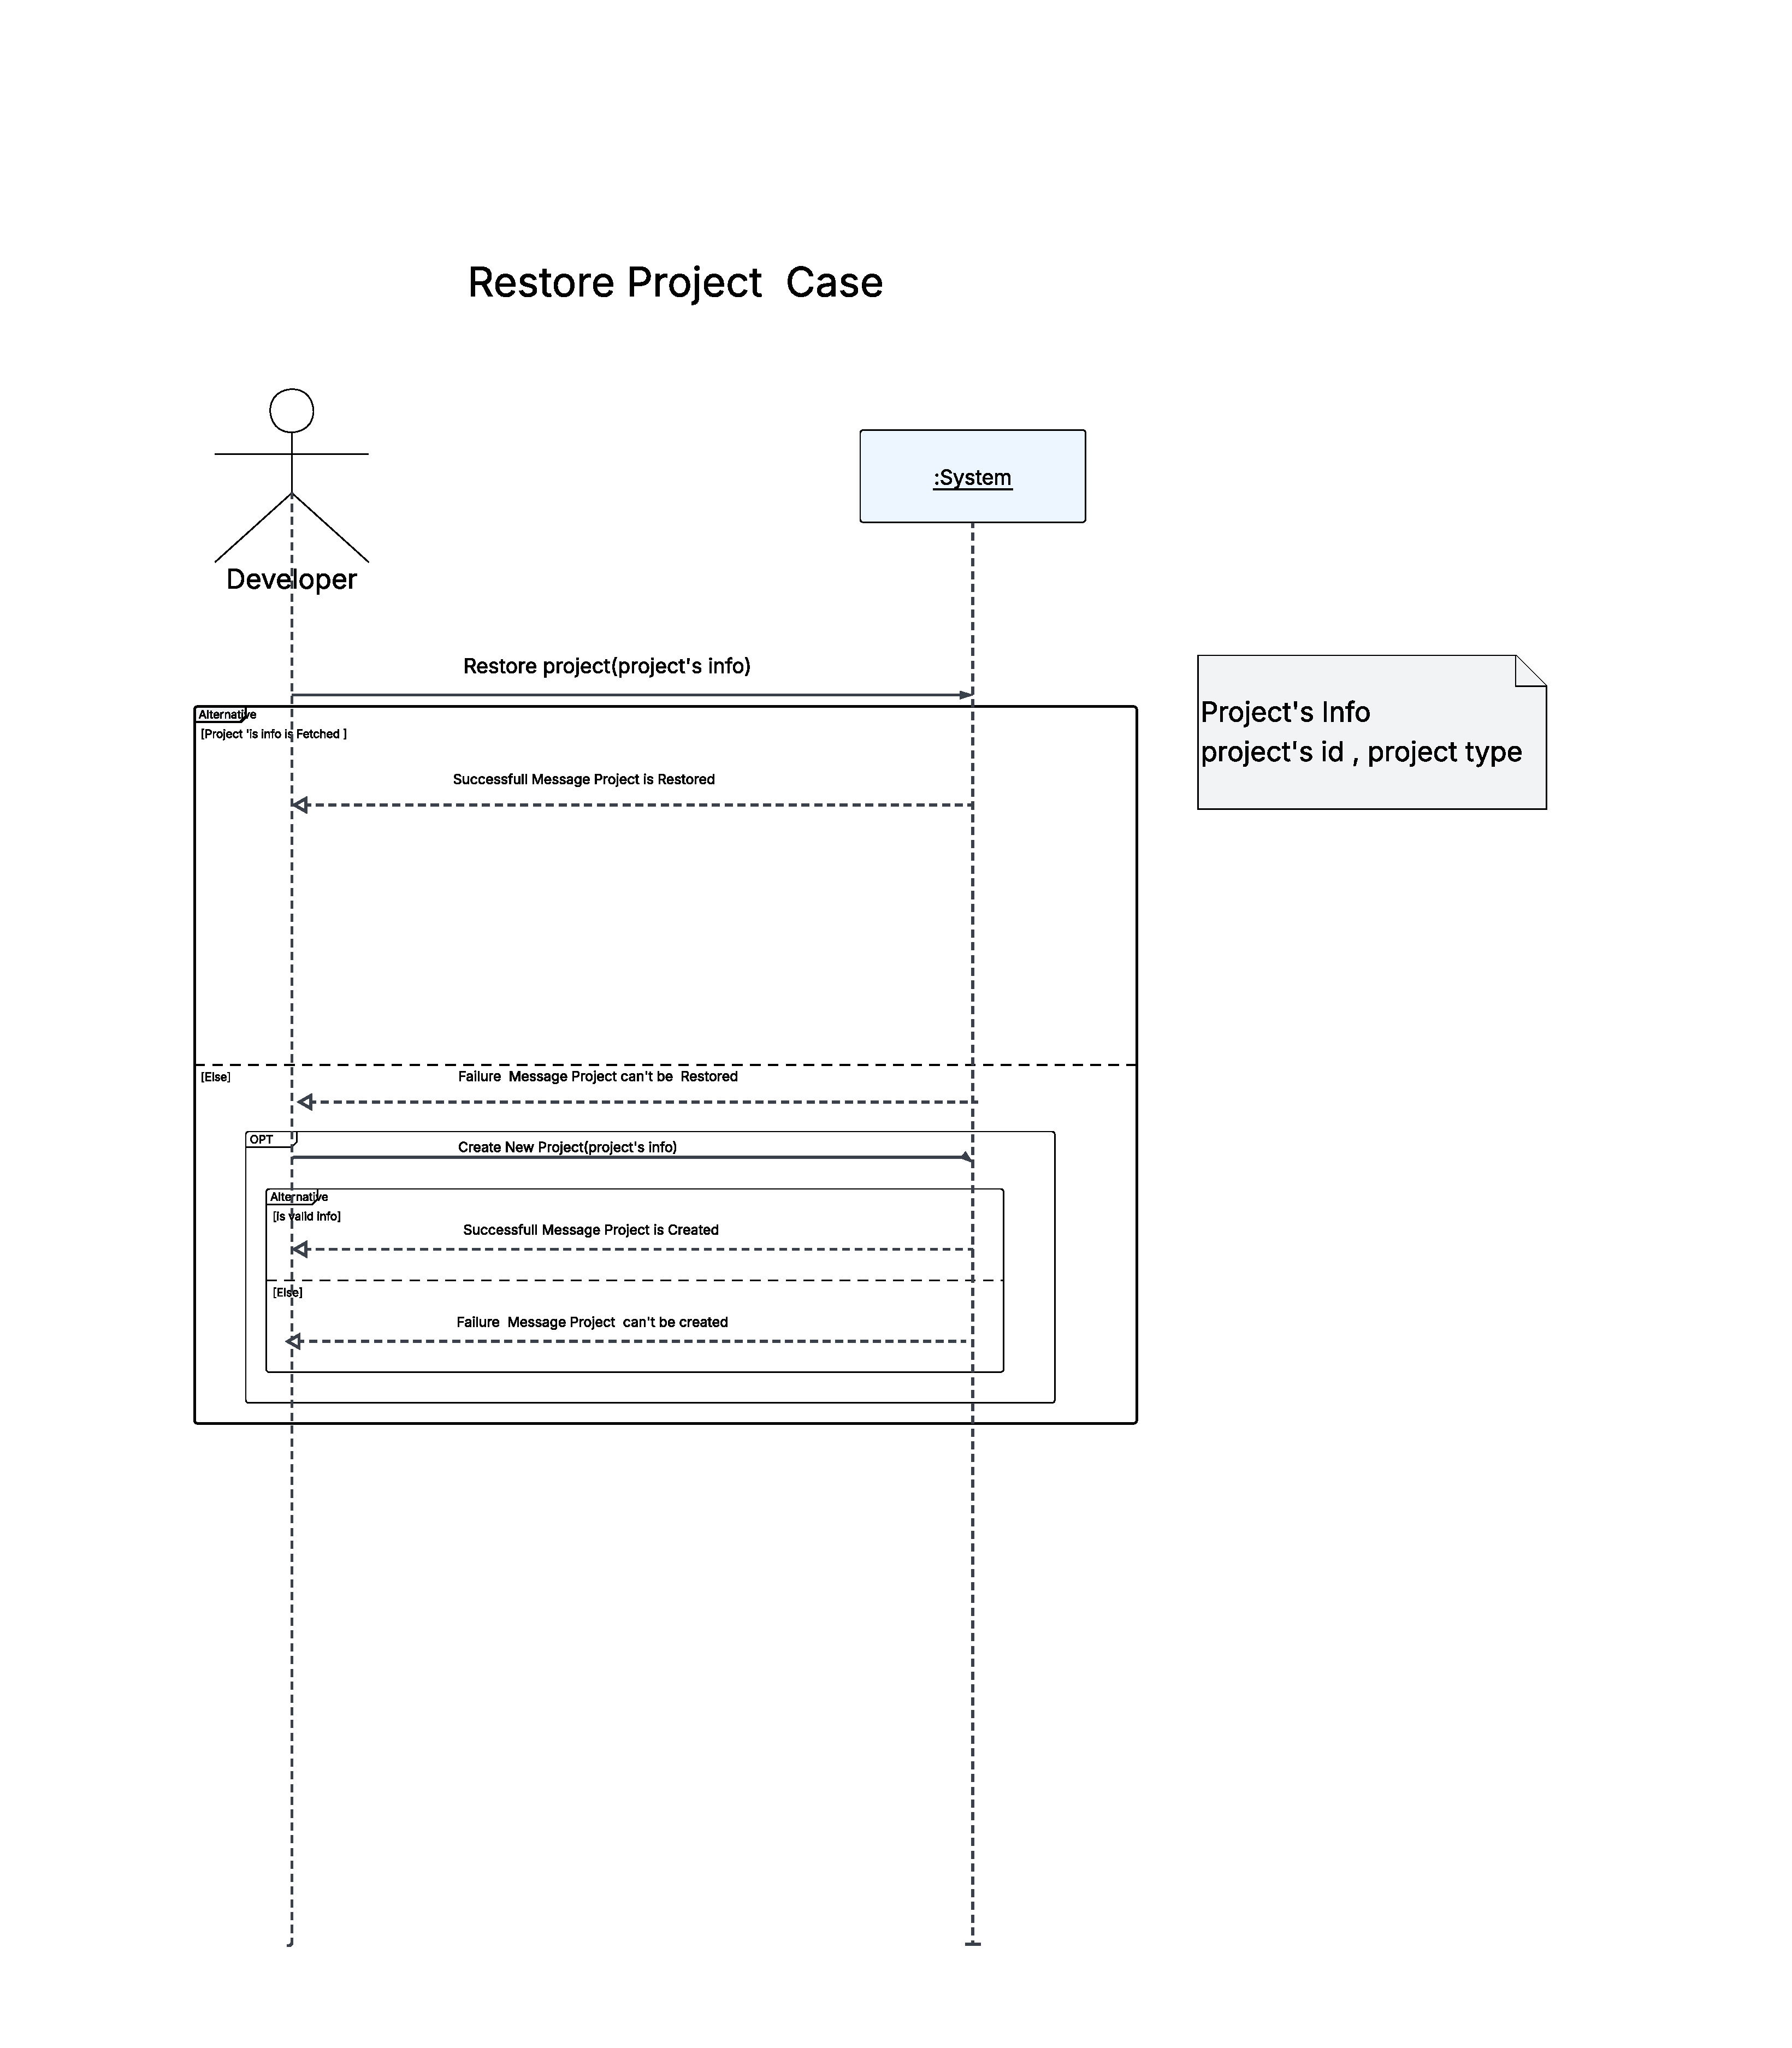
\includegraphics[width=\linewidth,height=0.9\textheight,keepaspectratio]{images/sequence/restore_project.pdf}
        \caption{Restore project sequence diagram}
        \label{fig:restore_project_sequence}
    \end{figure}
    
    \begin{figure}[H]
        \centering
        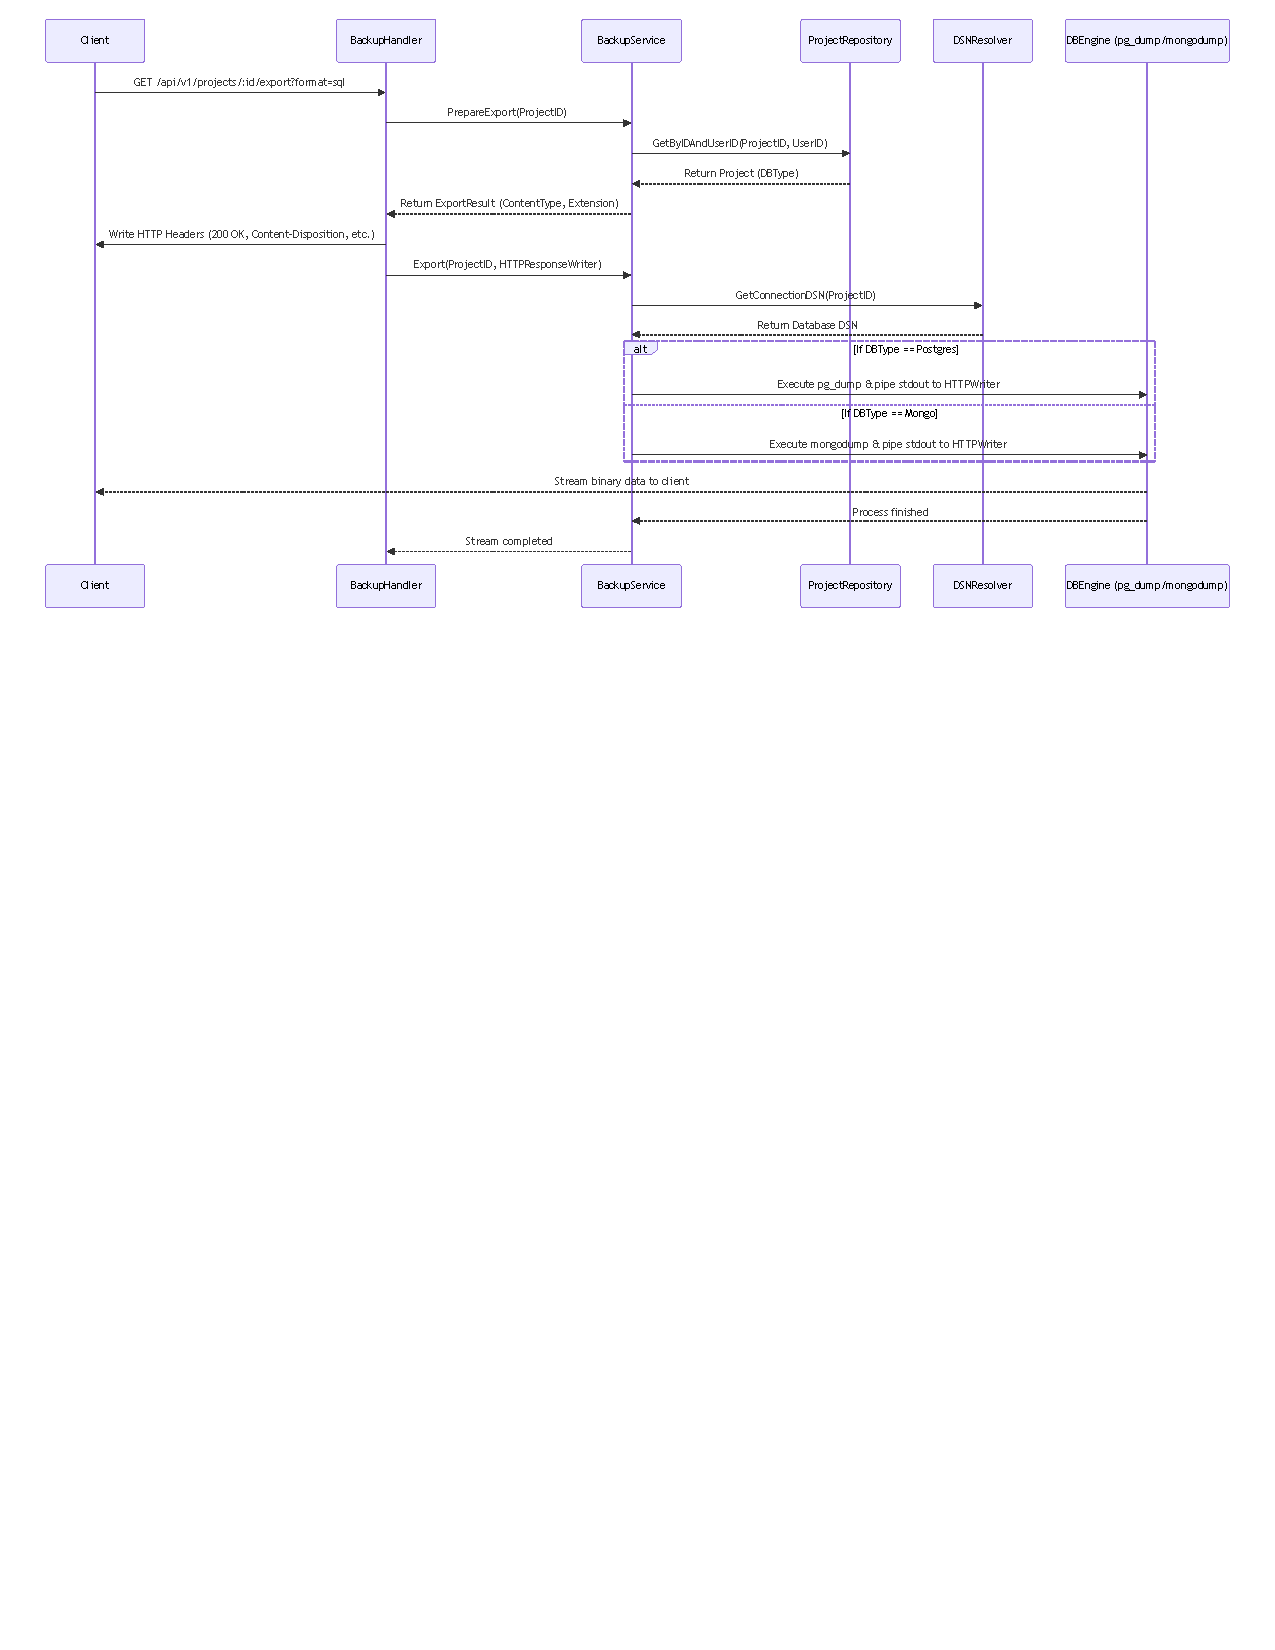
\includegraphics[width=\linewidth,height=0.9\textheight,keepaspectratio]{images/sequence/export_project.pdf}
        \caption{Export project sequence diagram}
        \label{fig:export_project_sequence}
    \end{figure}

    \begin{figure}[H]
        \centering
        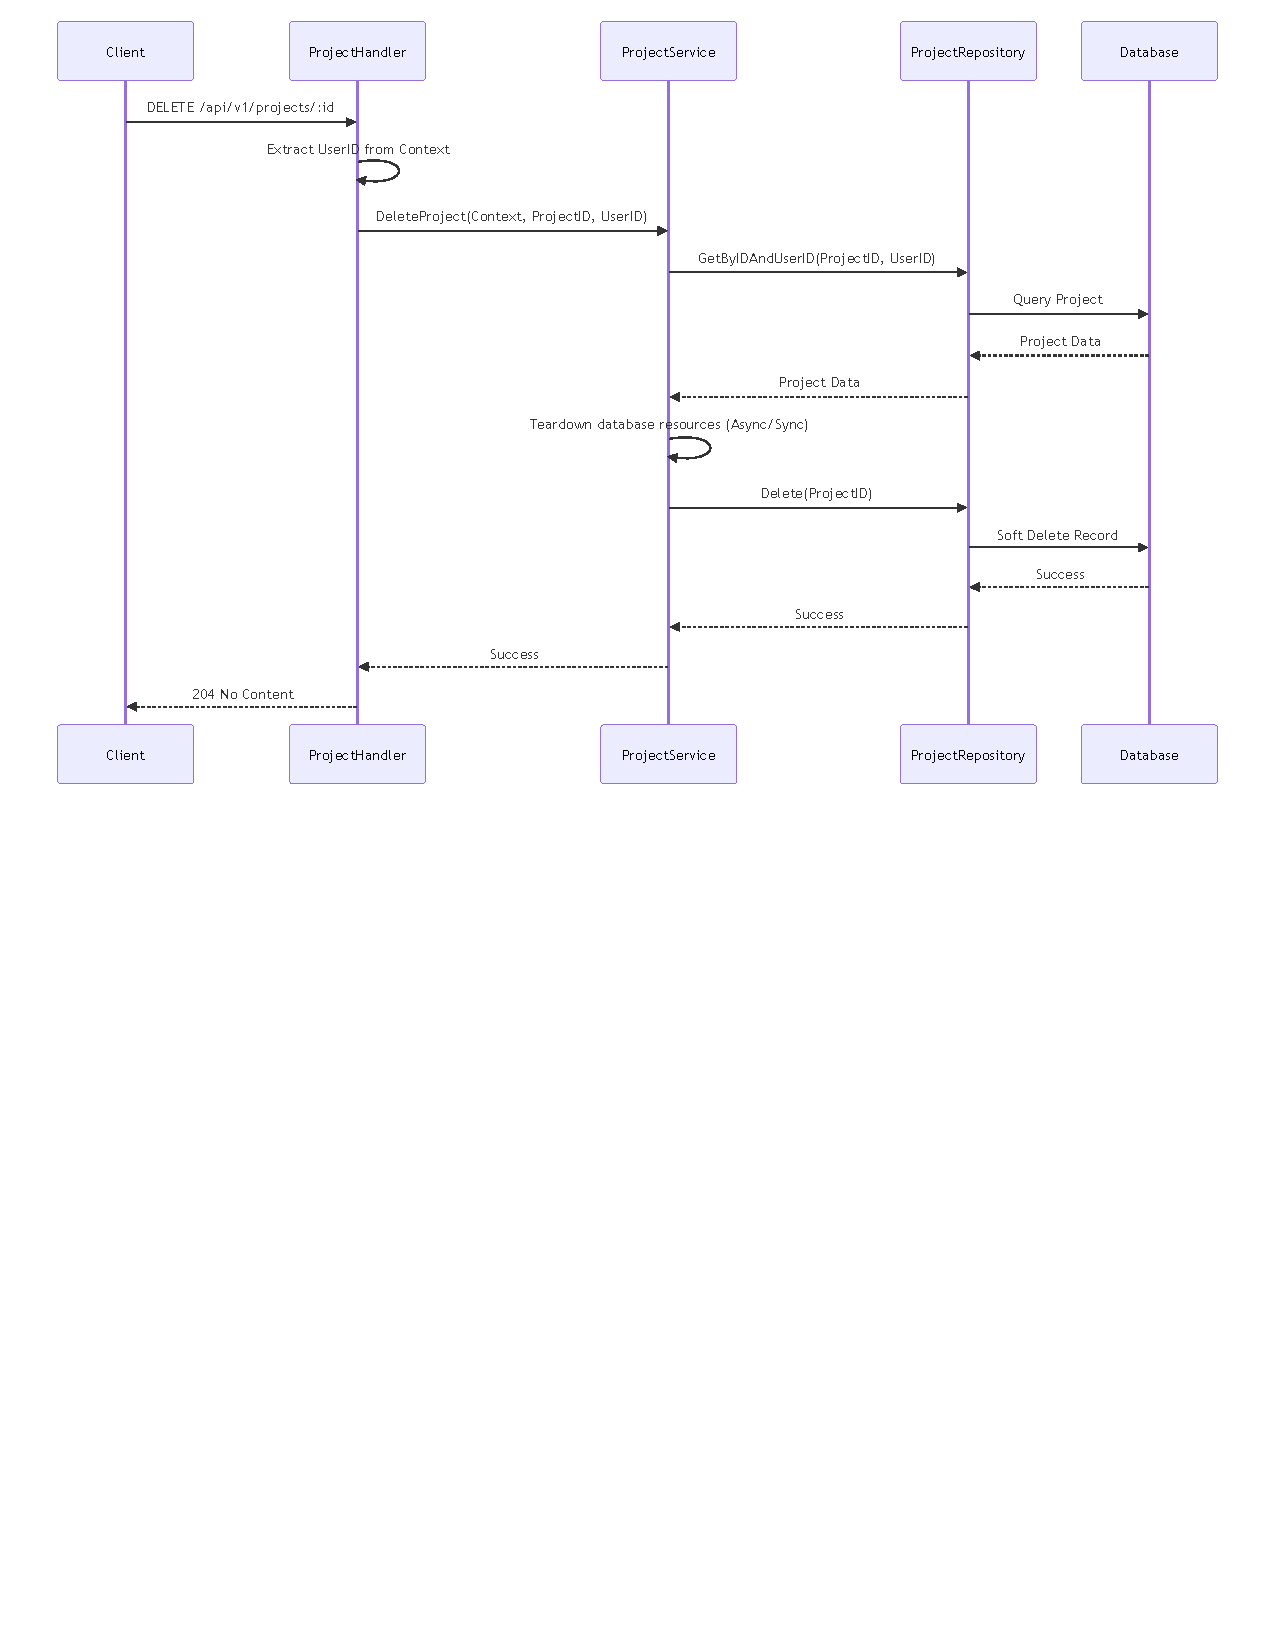
\includegraphics[width=\linewidth,height=0.9\textheight,keepaspectratio]{images/sequence/delete_project.pdf}
        \caption{Delete project sequence diagram}
        \label{fig:delete_project_sequence}
    \end{figure}

    \begin{figure}[H]
        \centering
        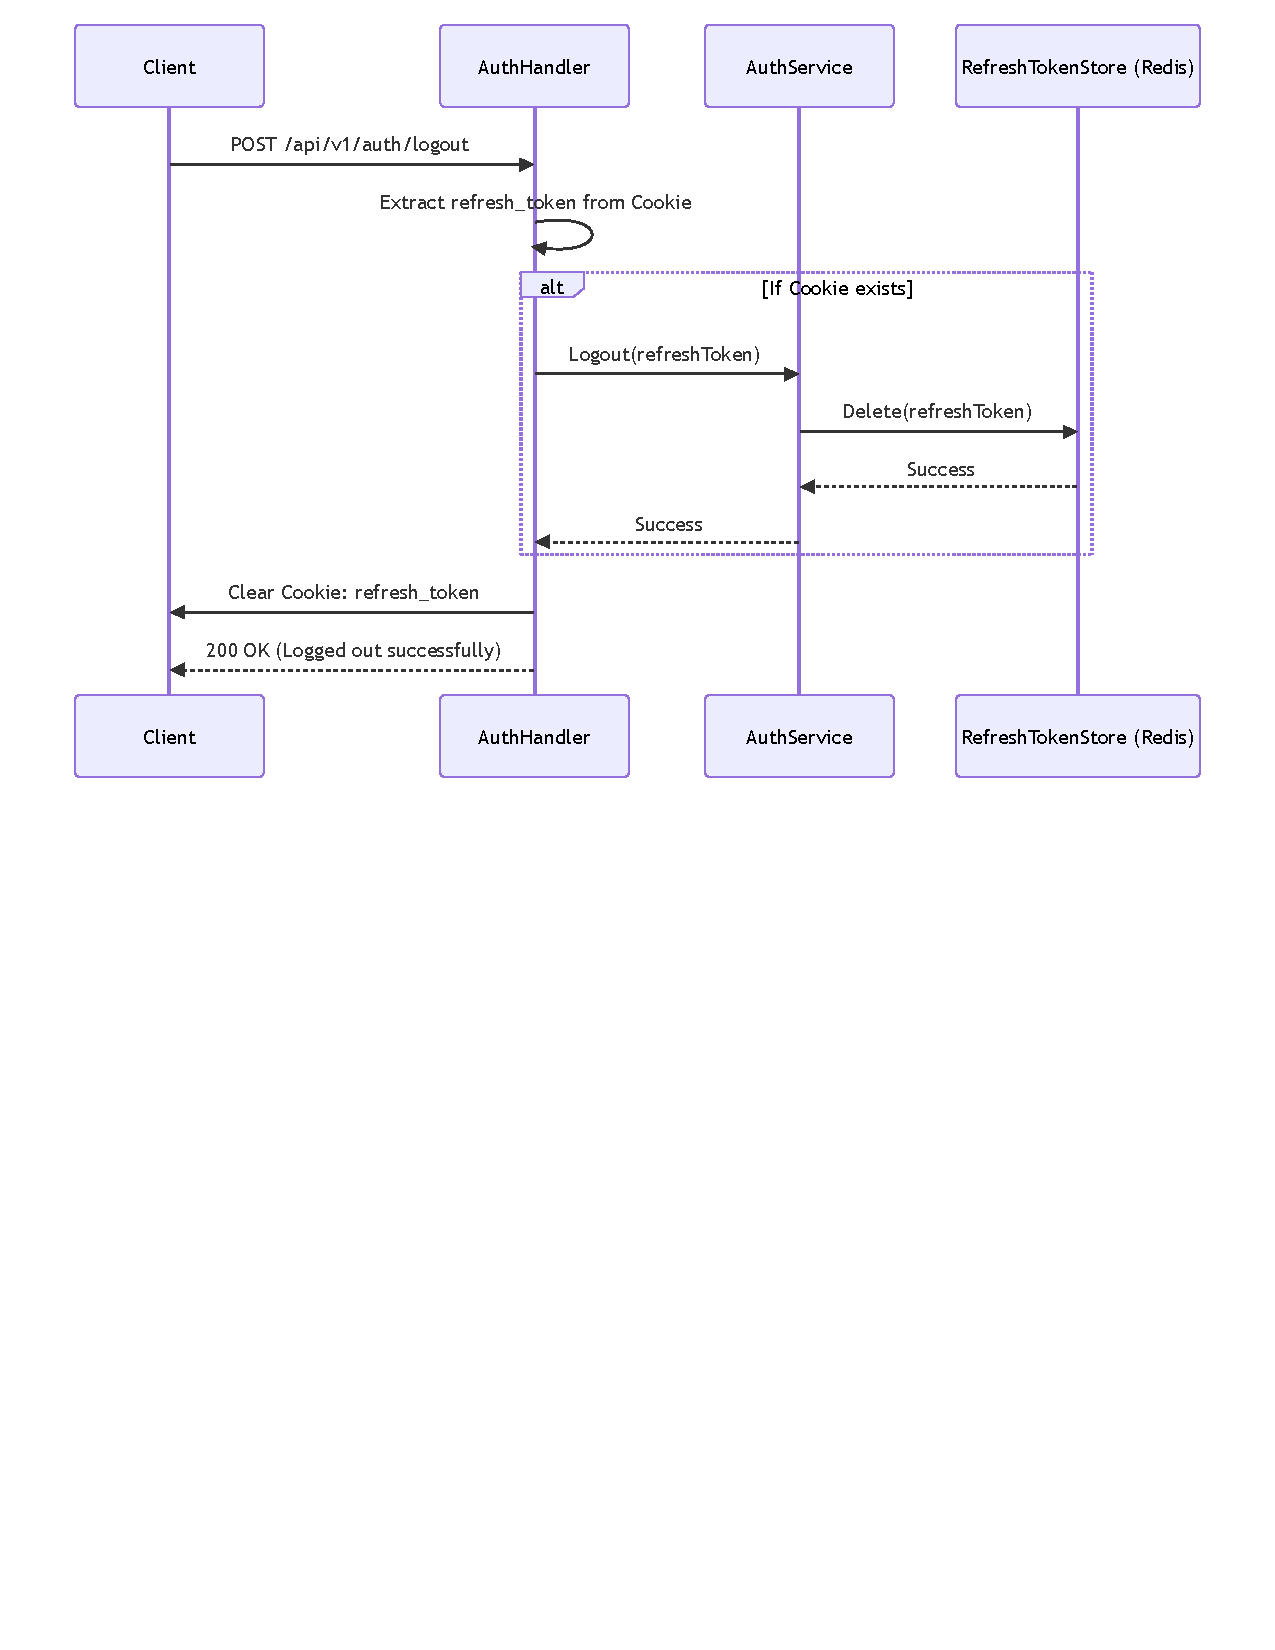
\includegraphics[width=\linewidth,height=0.9\textheight,keepaspectratio]{images/sequence/signout_seq.pdf}
        \caption{Signout sequence diagram}
        \label{fig:signout_sequence}
    \end{figure}